%%%%%%%%%%%%%%%%%%%%%%%%%%%%%%%%%%%%%%%%%%%%%%%%%%
% Basic setup. Most papers should leave these options alone.
\documentclass[fleqn,usenatbib]{mnras}

% MNRAS is set in Times font. If you don't have this installed (most LaTeX
% installations will be fine) or prefer the old Computer Modern fonts, comment
% out the following line
\usepackage{newtxtext,newtxmath}
% Depending on your LaTeX fonts installation, you might get better results with one of these:
%\usepackage{mathptmx}
%\usepackage{txfonts}

% Use vector fonts, so it zooms properly in on-screen viewing software
% Don't change these lines unless you know what you are doing
\usepackage[T1]{fontenc}

% Allow "Thomas van Noord" and "Simon de Laguarde" and alike to be sorted by "N" and "L" etc. in the bibliography.
% Write the name in the bibliography as "\VAN{Noord}{Van}{van} Noord, Thomas"
\DeclareRobustCommand{\VAN}[3]{#2}
\let\VANthebibliography\thebibliography
\def\thebibliography{\DeclareRobustCommand{\VAN}[3]{##3}\VANthebibliography}

%%%%% AUTHORS - PLACE YOUR OWN PACKAGES HERE %%%%%

% Only include extra packages if you really need them. Avoid using amssymb if newtxmath is enabled, as these packages can cause conflicts. newtxmatch covers the same math symbols while producing a consistent Times New Roman font. Common packages are:

%%% Math and symbols formatting %%% 
\usepackage{amsmath}	% Advanced maths commands
% \usepackage{amssymb}  % Advanced maths symbols
\usepackage{siunitx}    % SI units
\usepackage{pifont}     % Other symbols
\usepackage{upgreek}

%%% Figure formatting %%% 
\usepackage{graphicx}	% Including figure files
\usepackage{wrapfig}    % Enable wrapping text around figures
\usepackage{subcaption} % Enable cleaner subcaptions for subfigures

%%% Table formatting %%% 
\usepackage{booktabs}   % Create nicer tables
\usepackage{multirow}   % Enable multirow cells in tables

%%% Bibliography formatting %%% 
% \usepackage{natbib}
% \bibliographystyle{plainnat}

%%% Others formatting %%%
\usepackage{comment}
% \usepackage{float}
% \usepackage{setspace}

%%%%%%%%%%%%%%%%%%%%%%%%%%%%%%%%%%%%%%%%%%%%%%%%%%

%%%%% AUTHORS - PLACE YOUR OWN COMMANDS HERE %%%%%

% Please keep new commands to a minimum, and use \newcommand not \def to avoid
% overwriting existing commands. Example:
%\newcommand{\pcm}{\,cm$^{-2}$}	% per cm-squared
\newcommand{\Plus}{\mathord{\text{\ding{58}}}}


%%%%%%%%%%%%%%%%%%%%%%%%%%%%%%%%%%%%%%%%%%%%%%%%%%

%%%%%%%%%%%%%%%%%%% TITLE PAGE %%%%%%%%%%%%%%%%%%%

% Title of the paper, and the short title which is used in the headers.
% Keep the title short and informative.
\title[The Effects of Polydisperse Particle Distributions]{Planetesimal Formation from Pebble Cloud Collapse: The Effects of Polydisperse Particle Distributions}

% The list of authors, and the short list which is used in the headers.
% If you need two or more lines of authors, add an extra line using \newauthor
% 0009-0002-3268-2061
\author[V. M. Chhajed et al.]{
Vaibhav M. Chhajed,$^{1}$\thanks{E-mail: chhajedv@msu.edu}
Jackson T. Barnes,$^{2}$
and Seth A. Jacobson$^{1,2}$
\\
% List of institutions
$^{1}$Department of Physics and Astronomy, Michigan State University, 567 Wilson Road, East Lansing, MI, 48824, USA\\
$^{2}$Department of Earth \& Environmental Sciences, Michigan State University, 288 Farm Lane, East Lansing, MI 48824, USA\\
}

% These dates will be filled out by the publisher
\date{Accepted XXX. Received YYY; in original form ZZZ}

% Prints the current year, for the copyright statements etc. To achieve a fixed year, replace the expression with a number. 
\pubyear{\the\year{}}

% Don't change these lines
\begin{document}
\label{firstpage}
\pagerange{\pageref{firstpage}--\pageref{lastpage}}
\maketitle

% Abstract of the paper
\begin{abstract}
This is a simple template for authors to write new MNRAS papers.
The abstract should briefly describe the aims, methods, and main results of the paper.
It should be a single paragraph not more than 250 words (200 words for Letters).
No references should appear in the abstract.
\end{abstract}

% Select between one and six entries from the list of approved keywords.
% Don't make up new ones.
\begin{keywords}
keyword1 -- keyword2 -- keyword3
\end{keywords}

%%%%%%%%%%%%%%%%% BODY OF PAPER %%%%%%%%%%%%%%%%%%
\section{Introduction}\label{sec:Intro}

Planetesimals are the fundamental building blocks of planets. They form early in the evolution of protoplanetary disks and represent the first generation of solid bodies large enough for self-gravity to dominate their formation and subsequent evolution. 
These objects typically span sizes from a few kilometers to hundreds of kilometers and exhibit a wide range of shapes, spin states, and internal structures. 
Observations of asteroids, Kuiper Belt objects, and cometary nuclei reveal irregular morphologies, contact binaries, rubble-pile interiors, and significant porosity, all of which encode information about their formation pathways.
Understanding how such bodies form and acquire their physical properties is therefore central to theories of planet formation.

In protoplanetary disks, solid particles initially grow through collisional coagulation and produce aggregates ranging from micron-sized dust grains to mm- and cm-scale pebbles, which have been replicated in laboratory experiment and theoretical simulations.
However, growing to sizes larger than pebbles is difficult due to the effects of bouncing, which occurs when the mutual region of contact between pebbles is too small such that adhesion forces are inadequate for sticking at sufficiently high collision velocities that, and fragmentation, which occurs when the pebbles' internal strengths cannot withstand the stress of an even higher-velocity collision \citep[for a review of laboratory and theoretical simulation outcomes, see][]{Blum2018}.
Critically, the remaining pebbles will likely not experience the same collision again as a result of bouncing, and in the case of fragmentation, pebbles are largely destroyed; for both mechanisms growth is stymied at pebble sizes.

In the protoplanetary disk, a radial pressure gradient imposed by the Sun helps to support the disk's gas against the Sun's gravity, which in turn slows its orbit to sub-Keplerian velocities. 
Pebbles, which have settled to the protoplanetary disk midplane, continue to orbit at Keplerian velocities, and so they experience an headwind from the slower orbiting gas.
This imposed aerodynamic drag removes orbital energy from the pebbles, resulting in an inward radial drift toward the Sun \citep{Whipple1972,Weidenschilling1977,Hayashi1981}.
However, due to momentum feedback from the pebbles onto the gas, the gas drifts inward with the dust, and Coriolis accelerations then direct the gas from a radial to an azimuthal flow dragging the pebbles along with it.
This results in a super-Keplerian pebble velocity, pushing them radially outward onto wider orbits and creating local concentrations in so-called pebble clumps, which become increasingly more dense as the gas-dust interaction continues as a runaway process called the streaming instability \citep[see][for a review]{Squire2020}.
By accounting for the mutual aerodynamic coupling between gas and solids, streaming instability models demonstrated that small perturbations in particle density can grow exponentially, leading to the formation of dense filaments and clumps. 
Once these pebble clumps become sufficiently dense, they are no longer effected by external turbulence or stellar tidal forces \citep{Youdin2005b,Johansen2007b}.
Innumerable collisions between pebbles dissipates their kinetic energies and reduces their mutual collision velocities such that self-gravity dominates and the cloud collapses.
Subsequent numerical studies showed that when self-gravity is included, these overdense regions can collapse efficiently into bound kilometer-scale planetesimals on orbital timescales \citep{Johansen2015}. 
As the cloud collapses low-velocity collisions are more feasible and enable sticking, naturally resulting the rapid formation of kilometer-scale planetesimals directly from pebble-sized objects \citep{Johansen2015,Simon2024}.
Importantly, excess angular momentum retained from the aggregation of the pebble cloud is conserved during the collapse process, and so the cloud's rotation rate increases as its radius shrinks such that it exceeds the spin limit for a single planetesimal, and ultimately results in the creation of binary, triple, and higher multiplicity systems \citep{Nesvorny2010,Robinson2020,Barnes2025}. 

Planetesimals that formed from gravitational collapse would have likely preserved many of the attributes of their formation, including the orbits, compositions, shapes, and rotation states, and so we look to pristine small body populations as a means to constrain planetesimal formation conditions.
Approximately 30\% of objects in the cold classical Kuiper are members of binary systems \citep{Noll2020} on distinctly wide and low-inclination orbits \citep{Grundy2019}, and their components often exhibit similarly colored surfaces \citep{Fraser2021}.
Additionally, the lobes of the relict cold classical contact binary (486958) Arrokoth also exhibit similar color and albedo variations \citep{Stern2019,Grundy2020} across their surfaces, and its bilobed structure has been attributed to a low-velocity merger between mutually orbiting components \citep{Stern2019,McKinnon2020}.
These attributes have led to the hypotheses that cold classical Kuiper belt binaries formed together from a region of uniform composition and mild dynamics, key traits of a gravitationally collapsing pebble cloud.


\subsection{Prior Models of Gravitational Collapse}
% The formation of planetesimals through gravitational collapse has been studied extensively over the past decade, motivated by advances in both theory and numerical methods.
% Early models of planetesimal growth relied on incremental coagulation through pairwise sticking collisions.
% While successful at explaining the growth of micron-sized dust grains, these models encounter significant barriers at millimeter to meter scales, including rapid radial drift, bouncing, and fragmentation. 
% These challenges motivated the development of collective mechanisms capable of rapidly assembling large bodies.

Several key works have used N-body models to examine the gravitational collapse rotating clouds of super-particles as a mechanism to form planetesimal systems, and the results of their simulations have been highly successful in reproducing many observed properties of relict planetesimal systems in the asteroid and cold classical Kuiper belts \citep{Nesvorny2010,Robinson2020,Nesvorny2021,Barnes2025}.
The use of super-particles was necessitated by the infeasibility of directly modeling a real pebble cloud, which is theorized to contain approximately 10$^{21}$ cm-sized pebbles \citep{Johansen2014}.
With super-particles, the number of particles in the cloud can be scaled down to a more computationally feasible 10$^{5}$ particles, while their sizes are scaled up to km-sizes.
It is also expected that pebble clouds inherit excess angular momentum from their formation via the streaming instability \citep{Johansen2007b,Nesvorny2019}, and so gravitational collapse models from \citet{Nesvorny2010,Nesvorny2021}, \citet{Robinson2020}, and \citet{Barnes2025} modeled super-particle clouds with solid body rotation and varied their rotation rates to assess its affect on planetesimal system formation.
Employing this super-particle method, these simulations of gravitational collapse investigated a wide range of conditions for cloud collapse and their effects on the properties of fully formed planetesimal systems.

The results of gravitational collapse simulations from \citet{Nesvorny2010}, \citet{Robinson2020}, \citet{Nesvorny2021}, and \citet{Barnes2025} have been highly successful in reproducing many observed properties of relict planetesimal systems in the asteroid and cold classical Kuiper belts.
Nesvorn\'y et al. \citep{Nesvorny2010} first demonstrated that collapse-driven formation can reproduce the observed abundance of binary planetesimal systems, similar to those observed in the cold classical Kuiper belt \citep[e.g.,][]{Fraser2017,Grundy2019,Noll2020}.
\citet{Robinson2020} improved the treatment of particle collisions by employing smaller timesteps and refined collision handling, yielding more accurate dynamical evolution.
More recently, Barnes et al.~\citep{Barnes2025} used a soft-sphere discrete element method \citep[SSDEM;][]{Schwartz2012,Zhang2017} that allowed, for the first time, direct tracking of planetesimal shapes, spins, and internal structure during and following collapse.
Specifically, these prior models demonstrated a near 100\% binary planetesimal creation rate with many systems exhibiting near-equal masses ($m_2/m_1\gtrsim0.3$) and $\gtrsim$20\% of the initial cloud mass accreting to form the central and most massive planetesimal systems.
Moreover, they found that a sizeable fraction of planetesimals were components of wide binary systems that had binary semimajor axes which exceeded 7\% of their mutual Hill radius, as well as a smaller subpopulation of tightly orbiting binaries on dynamically cold orbits \citep{Robinson2020,Barnes2025}, similar to observed relict systems in the Kuiper belt \citep{Grundy2019,Noll2020}.
The mutual orbit inclinations of the simulated binary systems were also comparable to an observed $\sim$80\% prograde to $\sim$20\% retrograde split \citep{Barnes2025} as observed in the cold classical population \citep{Grundy2019} and modeled in streaming instability simulations \citep{Nesvorny2019}.
Together, these studies established gravitational collapse as a robust framework capable of matching many observed properties of small relict Solar System bodies.

It is important to note that although each of these gravitational collapse simulations successfully replicated many of the observed qualities of relict planetesimal systems, they were achieved with different numerical models netting unique results.
The simulations performed by \citet{Nesvorny2010,Nesvorny2021} and \citet{Robinson2020} relied on a perfect merger method, whereby colliding super-particles merge to create a planetesimal as a single large super-particle, and so planetesimals in their simulations formed as over-idealized spheres and had no recorded spin properties.
\citet{Barnes2025} employed an SSDEM to model planetesimals as aggregates of super-particles, and was therefore able to produce planetesimals that can experience both accretion and decretion and have tracked spins and distinct shapes, including bilobate objects similar to the contact binary (486958) Arrokoth \citep{Barnes2026}.
One notable result of the simulations from \citet{Barnes2025,Barnes2026} is that modeled planetesimals exhibit a pronounced increase in their spin rates with size for diameters in excess of $\sim$~100-km, which is strikingly comparable to the inflection in spin rates with diameter for observed asteroids, and suggest a potential primordial origin for the spin rates of large (D$\gtrsim$100-km) asteroids.
The smaller (D$\lesssim$100-km) observed asteroids and modeled planetesimals exhibit similar decreases in spin rates with size.
However, the asteroids rotate approximately 5 hours faster on average compared to the modeled planetesimals, which the authors attribute to the fact that these asteroids likely experienced significant collisional evolutions since their formation \citep{Harris1979,Bottke2015}.
The independent successes of these models strongly support gravitational collapse as a physically compelling mechanism for planetesimal formation.

While each of the previously noted numerical models of gravitational collapse have enabled a stronger understanding of this critical formation pathway, they chose to initialize their clouds with a monodisperse distribution of particles, whereby all particles had the same size and mass.
While this assumption simplifies the numerical problem and improves computational efficiency, it introduces several limitations that can strongly influence the formation and internal structure of modeled planetesimals.
Critically, with particles simulated as soft spheres, monodisperse systems favor symmetric packing arrangements, reduce the diversity of collision outcomes, and limit pathways for internal rearrangement and compaction. 
As a result, planetesimals created with soft-spheres exhibit uniform bulk densities and crystalline-like internal structures, which likely do not reflect the composition of real planetesimals \citep{Barnes2025}.
This crystal-locking effect suppresses internal rearrangement, limits shear-driven deformation, and leads to artificially uniform porosity and bulk density distributions.
Additionally, equal-mass collisions reduce the efficiency of angular momentum exchange and damp stochasticity in particle interactions, further constraining the range of attainable internal structures and spin states.
As a result, some properties produced by monodisperse collapse models may not reflect genuine physical outcomes. 
In contrast, real particle populations in protoplanetary disks are expected to span a wide range of sizes due to coagulation, fragmentation, and differential drift, leading to intrinsically polydisperse environments in which these numerical constraints are naturally alleviated.
Introducing particles of multiple sizes enables more efficient packing, as it allows for smaller grains to fill voids between larger particles, and enhances angular momentum redistribution during collapse.
These effects can significantly influence the dynamical and structural evolution of planetesimals, altering their bulk densities, internal porosity, shapes, spin rates, and propensity to form binary or multiple systems.
Polydispersity may also suppress artificial crystalline locking and produce a broader range of physically plausible outcomes, thereby improving the outcomes of prior gravitational collapse models.
The limitations of planetesimal formation imposed by monodisperse clouds motivates the need to extend gravitational collapse models to include polydisperse particle distributions. 

The absence of polydispersity therefore represents a critical oversimplification in current gravitational collapse models, and it must be investigated to determine whether the outcomes of previous simulations are robust predictions of gravitational collapse or if they are direct consequences of monodisperse distributions of super-particles. 
Astrophysical environments, by contrast, are inherently polydisperse.
Particles in protoplanetary disks undergo continuous growth, fragmentation, and radial sorting, which result in size distributions that span orders of magnitude, and it has been well-established that polydispersity is a key attribute of the streaming instability and it can directly affect the pebble clumping process \citep{Bai2010,Schaffer2018,Krapp2019,McNally2021,Rucska2023,Matthijsse2025}. 
% Laboratory experiments and numerical models have indicated that polydisperse particle populations pack more efficiently, redistribute angular momentum more effectively, and develop more heterogeneous internal structures than monodisperse assemblies. 
Because these pebble clumps are the progenitors of planetesimals, it is also likely that polydispersity will have some effect on the gravitational collapse process, which includes interparticle collisions, planetesimal growth, and final planetesimals' bulk densities, porosities, shapes, and spins.
Thus, in the following sections, we extend the framework used in \citet{Barnes2025} to investigate the consequences of polydisperse particle populations and use this improved model to systematically examine how particle-size diversity alters the dynamical and structural evolution of planetesimals formed through gravitational collapse.


\section{Methods}\label{sec:Methods}
The numerical framework used in this study follows the gravitational collapse methodology introduced by ~\citet{Barnes2025}, which employs the parallel $N$-body code PKDGRAV \citep[Parallel K-D Tree GRAVity;][]{Dikaiakos1996,Stadel2001,Richardson2000} together with its soft-sphere discrete element method \citep[SSDEM;][]{Schwartz2012,Zhang2017} to model the formation, internal structure, shapes, and spins states of planetesimals. 
PKDGRAV is a hierarchical tree-based gravity solver designed to efficiently compute gravitational interactions between large numbers of particles, and SSDEM augments this framework by resolving finite-duration particle contacts through spring–dashpot forces \citep{Schwartz2012,Zhang2017}. 
This combination allows the simultaneous treatment of long-range self-gravity and short-range collisional physics, making it well-suited for modeling dense clouds of particles.

In this work, we too perform numerical simulations of gravitational collapse using the PKDGRAV and its SSDEM, and we follow a similar framework as in \citet{Barnes2025} in that we simulate the collapse of self-gravitating super-particle clouds with near identical initial conditions (see \S~\ref{sec:simulations} in this paper).
However, the critical difference between our model and that of \citet{Barnes2025} is that we assess the consequences of polydisperse clouds on planetesimal formation, and we systematically compare our planetesimals with those that formed from monodisperse populations.
By incorporating polydispersity into our simulations of gravitational collapse, this work represents a critical step toward a better numerical representation of planetesimal formation via gravitational collapse. 
Without such advancements, it remains difficult to determine whether features such as crystalline interlocking and uniform bulk densities are true physical signatures or artifacts of oversimplified numerical assumptions. 

%% out of place in the methods section %%
% Our results demonstrate that particle-size diversity plays a central role in shaping the internal structure and evolution of planetesimals and should be considered an essential ingredient in future models of planet formation.
% The primary goal of this study is to quantify the effects of particle-size diversity on planetesimals' structures, spin states, and mutual orbit dynamics. 

% total cloud mass equivalent to a 100-km class planetesimal with a density of 1~$g/cm^3$, spatial extent, and initial rotation,

Because the physical basis of gravitational collapse, the numerical integrator, and the contact-force model are unchanged from \citet{Barnes2025}, we refer the reader to a detailed description of the PKDGRAV integrator, choices for the integration timestep and kinetic spring constant, collision detection, and interparticle restitution and frictional forces. 
Here, we summarize the elements necessary to understand our simulations and focus on the extensions introduced by incorporating polydisperse particle populations.


\subsection{Overview of the SSDEM}\label{sec:SSDEM}
The choice to use the SSDEM is motivated by its implementation of interparticle contact physics, which enables the creation of planetesimals as super-particle-aggregates with quantifiable shapes and spins. With the SSDEM, particles can overlap and experience mutual surface penetration, such that each particle is subject to static, rolling, and twisting frictional forces (\citealp{Schwartz2012,Zhang2017}; see \citealp{Barnes2025} for a review). Incident particles’ normal and tangential restoring forces are modeled as spring and dashpot systems, which require such input values as particle velocity, coefficient of dissipation, and overlap fraction, and these determine the amount of energy that is dissipated during a collision \citep{Cundall1978,Schwartz2012}. Restoring forces follow Hooke’s law such that all superparticle have an associated normal spring constant k$_\text{n}$, which determines the degree of overlap and the stiffness of a collision between two super-particles. It is critical to note, however, that the contact physics between super-particles merely represent inter-super-particle interactions and not real-world materials. In order to make direct comparisons with simulations from \citet{Barnes2025}, we followed their initial conditions set-up such that we too chose a spring constant k$_\text{n}\approx$~10$^{11}$~kg~s$^{-2}$, which corresponds with a simulation time step of about 4.7~s. These choices were made primarily due to the computational intensity of the SSDEM, but ultimately allowed for simulations to complete within approximately 1 month of wall-clock time.

\subsection{Initial Conditions and Implementation of Super-Particle Polydispersity}\label{sec:simulations}
Each simulation begins with a gravitationally bound cloud of solid particles, which represents one of the clumps produced by the streaming instability. 
The cloud is initialized with a fixed total mass corresponding to a 100-km class planetesimal with a density comparable to comets (1~g/cm$^3$).
The radius of the super particle cloud is set by the Hill radius, where $R_{\text{cloud}} = 0.6 R_{\text{Hill}}$, and $R_{\text{Hill}} = a_{\odot} (M_{\text{cloud}}/ 3 M_{\odot})^{1/3}$, $a_{\odot}$ is the heliocentric semi-major axis of cloud, $M_{\text{cloud}}$ is its total mass, and $M_{\odot}$ is the mass of the Sun.
As in \citet{Barnes2025}, our gravitational collapse simulations were performed at $a_{\odot}$~1~au so as to reduce the collapse timescale to a computationally feasible duration.
Moreover, because it expected that pebble clumps inherit rotation following their formation from the streaming instability \citep{Johansen2007b,Nesvorny2019} and the exact details of their rotation states are not known, we continue to simulate the rotations of our super-particle clouds as in \citet{Nesvorny2010}, \citet{Nesvorny2021}, \citet{Robinson2020}, and \citet{Barnes2025}, in which each cloud experiences solid body rotation governed by an initial rotation rate scale factor $f$ and the cloud angular velocity is calculated as $\Omega_{\text{cloud}} = f\Omega_{\text{circ}}$, where $\Omega_{\text{circ}} = (GM_{\text{cloud}}/R^3_{\text{cloud}})^{1/2}$ is the circular orbital frequency of a particle at the edge of the cloud.
Physically, it measures the ratio of rotational support to self-gravity. 
A rotation rate scale factor $f$ of zero corresponds to purely gravity-dominated collapse with no rotational support, and increasing values results in stronger centrifugal support.
As the parameter approaches unity, the centrifugal acceleration at the cloud boundary becomes comparable to gravitational acceleration, slowing radial contraction and promoting non-spherical deformation.
In this work, we consider five rotation rate scale factors ranging from $f\in$~[0.4, 1.2] in steps of 0.2, such that we sampled regimes of weak rotational support to cases in which rotation substantially modifies collapse dynamics.

The central objective of this work is to investigate how particle-size diversity influences the gravitational collapse, and so we needed to ensure that each cloud contained a sufficient variety of super-particle particle masses and radii to avoid any crystalline packing within resulting planetesimals.
Each cloud contains N$_{\text{SP}}$ = 10$^5$ super-particles such that each particle initially had identical masses M$_{\text{SP}}$ = M$_{\text{cloud}}$/N$_{\text{SP}}~\sim$~4.19~$\times$~10$^{13}$~kg and radii r$_{\text{SP}}~\sim$~2.15~km.
Polydispersity was implemented via a controlled mass dispersion, which was applied to the monodisperse particle distribution. 
Particle masses were scaled by randomly sampling multiplicative factors spanning the range $0.5\times$ to $1.5\times$ the initial monodisperse particle mass. 
Particle radii were then adjusted accordingly to preserve a uniform internal material density of 1~g/cm$^3$. 
Our implementation of polydispersity ensured that the total mass of the collapsing cloud remained identical to the monodisperse case while introducing systematic size diversity for each particle and eliminating crystalline packing.

Each cloud's polydisperse size distribution contains a large number of smaller particles that dominate the particle population and a smaller population of larger particles that contribute a disproportionate fraction of the mass and gravitational influence within the collapsing cloud. 
%The distribution is truncated to avoid particles that are either too small to be reliably resolved by the numerical model or so large that they dominate local collapse dynamics. 
The distribution is truncated to avoid particles that are either too small to contribute meaningfully to the gravitational dynamics of the collapsing cloud, or so large that they dominate local collapse dynamics.
Aside from the particle-size distribution itself, all other initial conditions remain identical to those used in the monodisperse simulations: the total cloud mass, the initial spatial extent of the particle cloud, the imposed rotation rate scale factor, particle material densities, and the gravitational and contact-force prescriptions governing particle interactions \citep[as described in][]{Barnes2025}.
This design ensures that any differences observed between the monodisperse and polydisperse simulation suites can be attributed solely to the introduction of particle-size diversity.

\begin{table*}
    \centering
    \caption{Parameters describing the SSDEM $N$-body simulations conducted for this work and in \citet{Barnes2025}. The polydisperse suite samples particle masses uniformly from $0.5\times$--$1.5\times$ the monodisperse particle mass, with radii adjusted to preserve a uniform material density of 1\,g\,cm$^{-3}$, ensuring the total cloud mass remains identical to the monodisperse case.}
    \label{tab:particle_setup}
    \begin{tabular}{ccccccc|ccccccc}
        \hline
        \multicolumn{7}{c|}{\textit{Suite 1 -- Monodisperse Angular Velocity \citep{Barnes2025}}} &
        \multicolumn{7}{c}{\textit{Suite 3 -- Polydisperse Angular Velocity (This work)}} \\
        \hline
        $f$ & $\varepsilon_{n}$ & $\varepsilon_{t}$ & $\mu_{s}$ & $\mu_{r}$ & $\mu_{t}$ & Runs &
        $f$ & $\varepsilon_{n}$ & $\varepsilon_{t}$ & $\mu_{s}$ & $\mu_{r}$ & $\mu_{t}$ & Runs \\
        \hline
        0.2 & 0.5 & 1.0 & 0.0 & 0.0 & 0.0 & 5 & \multicolumn{7}{c}{} \\
        0.4 & 0.5 & 1.0 & 0.0 & 0.0 & 0.0 & 5 & 0.4 & 0.5 & 1.0 & 0.0 & 0.0 & 0.0 & 5 \\
        0.6 & 0.5 & 1.0 & 0.0 & 0.0 & 0.0 & 5 & 0.6 & 0.5 & 1.0 & 0.0 & 0.0 & 0.0 & 5 \\
        0.8 & 0.5 & 1.0 & 0.0 & 0.0 & 0.0 & 5 & 0.8 & 0.5 & 1.0 & 0.0 & 0.0 & 0.0 & 5 \\
        1.0 & 0.5 & 1.0 & 0.0 & 0.0 & 0.0 & 5 & 1.0 & 0.5 & 1.0 & 0.0 & 0.0 & 0.0 & 5 \\
        1.2 & 0.5 & 1.0 & 0.0 & 0.0 & 0.0 & 5 & 1.2 & 0.5 & 1.0 & 0.0 & 0.0 & 0.0 & 5 \\
        \hline
        \multicolumn{7}{c|}{\textit{Suite 2 -- Monodisperse Contact Physics \citep{Barnes2025}}} &
        \multicolumn{7}{c}{\textit{Suite 4 -- Polydisperse Contact Physics (This work)}} \\
        \hline
        $f$ & $\varepsilon_{n}$ & $\varepsilon_{t}$ & $\mu_{s}$ & $\mu_{r}$ & $\mu_{t}$ & Runs &
        $f$ & $\varepsilon_{n}$ & $\varepsilon_{t}$ & $\mu_{s}$ & $\mu_{r}$ & $\mu_{t}$ & Runs \\
        \hline
        0.4 & 0.5 & 0.5 & 0.0 & 0.0 & 0.0 & 3 & 1.0 & 0.5 & 0.5 & 0.0 & 0.0 & 0.0 & 5 \\
        0.4 & 0.5 & 0.5 & 0.5 & 0.5 & 0.5 & 3 & 1.0 & 0.5 & 0.5 & 0.5 & 0.5 & 0.5 & 5 \\
        0.4 & 0.9 & 0.9 & 0.0 & 0.0 & 0.0 & 3 & 1.0 & 0.5 & 0.5 & 1.0 & 1.0 & 1.0 & 5 \\
        0.4 & 0.9 & 0.9 & 0.5 & 0.5 & 0.5 & 3 & 1.0 & 0.5 & 0.5 & 2.0 & 2.0 & 2.0 & 5 \\
        1.0 & 0.5 & 0.5 & 0.0 & 0.0 & 0.0 & 3 & 1.0 & 0.7 & 0.7 & 0.0 & 0.0 & 0.0 & 5 \\
        1.0 & 0.5 & 0.5 & 0.5 & 0.5 & 0.5 & 3 & 1.0 & 0.7 & 0.7 & 0.5 & 0.5 & 0.5 & 5 \\
        1.0 & 0.9 & 0.9 & 0.0 & 0.0 & 0.0 & 3 & 1.0 & 0.7 & 0.7 & 1.0 & 1.0 & 1.0 & 5 \\
        1.0 & 0.9 & 0.9 & 0.5 & 0.5 & 0.5 & 3 & \multicolumn{7}{c}{} \\
        \hline
    \end{tabular}
    \newline
    \vspace{4pt}
    \begin{minipage}{\linewidth}
        \small\textit{Note.} Each simulation suite is defined by the initial cloud rotation rate scale factor ($f$); coefficients of normal ($\varepsilon_n$) and tangential ($\varepsilon_t$) restitution; coefficients of static ($\mu_s$), rolling ($\mu_r$), and twisting ($\mu_t$) friction; and the total number of runs per parameter combination (\textit{Runs}). For Suites 1 and 2, all particles have identical masses and radii \citep{Barnes2025}. For Suites 3 and 4, particle masses are sampled uniformly from $0.5\times$--$1.5\times$ the monodisperse particle mass with radii adjusted to preserve a uniform material density of 1\,g\,cm$^{-3}$.
    \end{minipage}
\end{table*}

% Having described the gravitational and contact framework used to evolve collapsing particle clouds, we now outline the initial conditions and simulation design adopted in this study.
% In particular, we introduce the dimensionless rotation parameter used to characterize the cloud’s initial angular momentum, describe the two particle-size suites considered (monodisperse and polydisperse), and summarize the ensemble of realizations analyzed. These elements establish the parameter space over which we later compare structural and dynamical outcomes.

We ran four simulation suites that were initialized with different particle distributions and contact physics parameters, as summarized in Table~\ref{tab:particle_setup}.
Suite 1 and Suite 3 investigate the effects of cloud rotation rate by varying $f \in [0.2, 1.2]$ in steps of 0.2 for the monodisperse case \citep{Barnes2025} and $f \in [0.4, 1.2]$ in steps of 0.2 for the polydisperse case, while maintaining nominal contact physics parameters ($\varepsilon_n = 0.5$, $\varepsilon_t = 1.0$, $\mu_s = \mu_r = \mu_t = 0.0$).
Suite 2 and Suite 4 instead fix the rotation rate at $f = 1.0$ for the polydisperse case and vary $f = 0.4$ or $1.0$ for the monodisperse case \citep{Barnes2025}, and vary the coefficients of restitution and friction to investigate the role of interparticle contact physics.
For each parameter combination in the angular velocity suites, five unique super-particle clouds were generated using different random seeds to produce random but spatially uniform particle distributions within the cloud.
For the monodisperse contact physics suite \citep{Barnes2025}, three runs were performed per parameter combination, while five runs were performed for each polydisperse contact physics combination.
In total, 30 monodisperse angular velocity simulations, 24 monodisperse contact physics simulations \citep{Barnes2025}, 25 polydisperse angular velocity simulations, and 35 polydisperse contact physics simulations were analyzed, yielding 114 simulations in total.
While the rotation rate scale factors, contact physics parameters, and collision schemes are identical across runs within each suite, the resulting compaction histories and aggregate structures differ systematically between rotation states, contact physics parameters, and between monodisperse and polydisperse suites.

\begin{comment}
\subsection{Simulation Execution and Analysis Pipeline}
Each simulation is evolved until large-scale dynamical activity subsides and the collapsing cloud settles into stable gravitationally bound aggregates. In practice, this corresponds to several dynamical times of the initial cloud and typically requires integration over a timescale comparable to the full collapse and relaxation of the system. During this evolution, the collapse proceeds through two broad stages: an initial phase of rapid global contraction driven by self-gravity, followed by a slower relaxation phase in which particles undergo repeated collisions, dissipate kinetic energy, and rearrange within the forming aggregates. This latter stage allows the system to approach mechanical equilibrium as particle contacts stabilize and internal structure develops.This takes one and half year in simulation time.

Final planetesimals are identified using the clump-finding procedure described by \citet{Barnes2025}, which groups particles into gravitationally bound objects based on their mutual gravitational binding energy and relative kinematics. For each identified planetesimal, we compute several physical and dynamical properties. The total mass of the aggregate is obtained by summing the masses of all constituent particles. The rotation period is derived from the aggregate’s net angular momentum and moment of inertia, treating the body as a rigidly rotating system once the collapse has stabilized. Shape parameters are calculated from the eigenvalues of the inertia tensor, which provide estimates of the principal axes of the aggregate and allow characterization of its overall geometry (e.g., oblate, prolate, or triaxial).

For systems that form multiple bound aggregates, we identify binary or higher-order configurations and compute their mutual orbital properties. Orbital separation is determined from the relative positions of the component centers of mass, while eccentricity and inclination are derived from the relative orbital angular momentum and energy of the system. These quantities characterize the dynamical architecture of bound systems produced during collapse and allow comparison with observed properties of small-body binaries in the Solar System.

In the polydisperse simulations, additional diagnostics are applied to quantify the internal organization of particle sizes within each aggregate. These analyses measure the degree of size sorting that occurs during collapse and track the spatial distribution of particles of different sizes within the final planetesimal structure. Such diagnostics help assess how particle-size diversity influences compaction, internal structure, and the redistribution of mass during gravitational collapse.
\end{comment}

\subsection{Bulk Density Estimation Using Voxel-Based Volume Reconstruction}\label{sec:bulk_density}
To estimate the bulk densities of the planetesimals produced in our simulations, it is necessary to determine the physical volume occupied by each gravitationally bound aggregate.
This task is non-trivial because bodies formed through gravitational collapse are typically irregular in shape and may contain internal voids produced during their accretion and subsequent particle rearrangement. 
Simple geometric approximations---such as assuming that each aggregate is spherical or estimating its volume using a convex hull---can introduce systematic biases because they ignore concave surface features and internal porosity present in the final planetesimals.
To avoid these assumptions, we reconstruct the aggregate volume using a voxel-based geometric method that directly measures the spatial region occupied by its constituent particles.

For each identified planetesimal, we extract the spatial coordinates, masses, and radii of its constituent particles.
The physical space occupoed by each particle is then discretized into a uniform three-dimensional grid of cubic voxels with fixed spatial resolution. 
Each particle is mapped to a voxel index according to its position, and any voxel containing at least one particle is classified as occupied. 
The enclosing volume of the aggregate is computed by summing the volumes of all occupied voxels, providing a resolution-controlled approximation of the spatial region occupied by the planetesimal.
In this work, we adopt a voxel size of 4.5~km. This resolution is small compared to the characteristic size of many $\gtrsim$40~km class planetesimals produced in our simulations, and so it enables the capture of irregular boundaries and concave surface features while remaining computationally efficient.

Because the number of constituent particles varies widely across our planetesimals, different numerical strategies are employed to identify unique occupied voxels depending on system size: direct enumeration is used for smaller aggregates, whereas spatial indexing techniques are applied to larger systems to identify unique voxels efficiently.
Once the enclosing volume is determined, the bulk density of each planetesimal is calculated as the ratio of the total particle mass to the reconstructed volume. 
We also compute the packing efficiency, defined as the ratio of the summed intrinsic volumes of the constituent particles to the enclosed volume, which provides a complementary measure of internal porosity.
This voxel-based reconstruction yields consistent, resolution-controlled estimates of bulk density for aggregates of varying size and morphology and enables direct comparison between the planetesimals created from monodisperse distributions \citep[i.e.,][]{Barnes2025} and those that are created from polydisperse  distributions and are analyzed in this work.

\section{Results}\label{sec:results}
The results presented here build upon those of \citet{Barnes2025} by extending the analysis to particle populations that include both monodisperse (uniform-size) and polydisperse (size-diverse) distributions. 
To guide the discussion, we first examine behaviors that remain consistent between these two particle populations—those primarily governed by global gravitational collapse and angular momentum evolution, rather than the details of particle-size variation. 
We then highlight cases in which particle-size diversity introduces measurable physical differences, altering the internal structure, spin properties, and binary formation efficiency of the resulting planetesimals. 

This organization, moving from shared to divergent behavior between monodisperse and polydisperse particle populations, allows us to distinguish outcomes that are intrinsic to gravitational collapse from those that depend on the size distribution of the constituent particles. Section~\ref{sec:shared} focuses on shared properties such as the spin–size and shape–spin relations, which are nearly identical for both particle populations. Section~\ref{sec:different} then examines properties that differ between the monodisperse and polydisperse cases, including bulk density, rotation period distributions, and binary statistics, as well as morphological and orbital variations. Finally, Section~\ref{sec:friction_effects} isolates the role of interparticle friction within the polydisperse population, demonstrating how material strength further influences the stability and final shapes of the formed bodies.

\subsection{Shared Trends Between Monodisperse and Polydisperse Systems}\label{sec:shared}
\subsubsection{Spin-Size relationship}

\begin{comment}
Figure~\ref{fig:spin_v_diameter} shows the relationship between planetesimal size and rotation rate resulting from gravitational collapse, alongside observational constraints from main-belt asteroids and Kuiper Belt objects. Rather than simply illustrating the distribution of simulated bodies, this figure highlights how rotation emerges as a function of both object size and the initial angular momentum of the collapsing cloud. 

Across both particle-size models, a clear trend is visible in which smaller bodies exhibit a wider spread in rotation rates, while larger planetesimals tend to cluster toward slower spins. This behavior reflects the redistribution of angular momentum during collapse, where interactions and mergers act to regulate the final rotation states. The inclusion of observational data provides an important benchmark, allowing direct comparison between simulated outcomes and real small-body populations.

The distinction between monodisperse and polydisperse particle populations becomes more evident when examining the detailed structure of the distribution, which we explore further in the following paragraphs. In particular, deviations in spin distributions and their dependence on size provide insight into how particle-scale physics influences the macroscopic evolution of planetesimals.

%Figure~\ref{fig:spin_v_diameter} illustrates how rotation rates of planetesimals formed through gravitational collapse depend on their final size and the initial spin of their parent clouds. 
%The x-axis, ``Diameter (km),'' represents the size of each planetesimal, while the y-axis, ``Spin Rate (rev/day),'' shows how fast each object rotates. 
%Both axes are plotted on logarithmic scales to capture the broad range of values. 
%Gray points correspond to observational data for small bodies in the solar system main belt asteroids  and Kuiper Belt Objects/Trans-Neptunian Objects (pluses)—while the colored points represent simulation results. Triangles mark monodisperse (Mono) systems, and circles represent polydisperse (Poly) ones. The color gradient indicates the initial cloud rotation rate, with lighter shades corresponding to faster initial spin. 


A clear inverse trend between spin rate and diameter is visible: smaller planetesimals generally rotate faster than larger ones, consistent with angular momentum conservation during collapse. 
This behavior is seen in both Monodisperse and Polydisperse populatiobserved in both Monodisperse and Polydisperse populations and is consistent with the distribution of observed solar system objects, in which small planetesimals often spin several times per day, whereasween simulation and observational data suggests that gravitational collapse models can reproduce realistic(change this) spin characteristics. 
%The spread in spin rates among similar-sized bodies largely reflects differences in the initial rotation rate of their parent clouds, as shown by the color variation. 
At diameters above roughly 100~km, the data cluster below one revolution per day, implying that self-gravity imposes an upper limit on rotation rate—faster-spinning bodies would become structurally unstable. 

When comparing Mono and Poly systems, both populations follow nearly identical overall trends, though Poly systems exhibit slightly more scatter, particularly at intermediate sizes. 
This variation likely arises from irregular angular momentum redistribution during collapse, as polydisperse particle mixtures introduce additional dynamical complexity. 
Nevertheless, both systems converge toward a similar spin-rate boundary at small sizes, reinforcing that gravitational collapse naturally produces realistic spin–size relationships largely independent of particle size uniformity. 
Extrapolating these trends suggests that the observed correlation between size and rotation among small Solar System bodies can arise directly from the collapse of rotating clouds, with the initial cloud spin setting the envelope of final rotation rates. 
These results support the idea that planetesimal spins retain a dynamical memory of their formation conditions, even after billions of years of evolution.
\end{comment}

\begin{figure*}
    \centering
    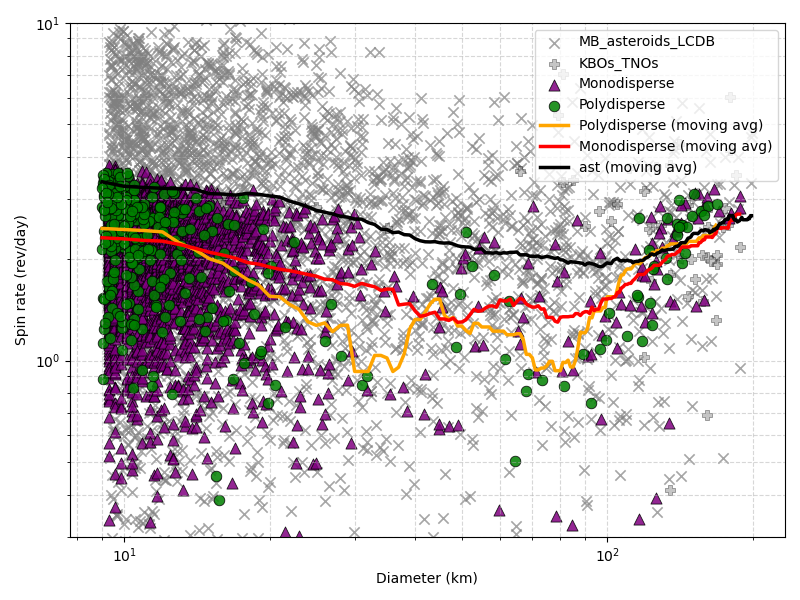
\includegraphics[width=\textwidth]{figures/spin_rate_dia (1).png}
    \caption{The planetesimal spin rates (rev. day$^{-1}$) relative to their their sizes (km). 
    Observations of main belt asteroids are shown with a gray $\times$ symbol and TNOs are shown with a $\Plus$ symbol. 
    Circles represent polydisperse planetesimals, and triangles represent monodisperse planetesimals. 
    % The color of each point indicates the initial spin of the cloud they formed from (rotation rate factor f), with brighter colors meaning faster initial rotation.
    }
    \label{fig:spin_v_diameter}
\end{figure*}

Figure~\ref{fig:spin_v_diameter} shows the relationship between planetesimal size and rotation rate resulting from gravitational collapse, alongside observational constraints from main-belt asteroids and Kuiper Belt objects. 
Rather than simply illustrating the distribution of simulated bodies, this figure highlights how rotation depends on both object size and the angular momentum evolution during collapse.

Across both particle-size models, a clear non-monotonic trend is visible. Small bodies ($\sim 10$ km) exhibit a wide spread in spin rates, with many rotating relatively quickly.
As size increases toward intermediate scales ($\sim 30$--$60$ km), the average spin rate decreases, reaching a minimum.
For larger bodies ($\gtrsim 100$ km), the spin rate begins to increase again, as shown by the moving average curves.
This produces a characteristic ``dip'' in the spin--size relation that is not captured by a simple inverse scaling.

This behavior reflects the complex redistribution of angular momentum during collapse. 
At small sizes, fragments retain a large fraction of their initial angular momentum, leading to rapid and highly scattered rotation rates.
At intermediate sizes, collisions and mergers redistribute angular momentum more efficiently, reducing the net spin. 
At larger sizes, the re-accumulation of material and coherent rotation of the merged body leads to a modest increase in spin rate.

The inclusion of observational data provides an important benchmark.
The simulated distributions overlap significantly with the observed asteroid populations, particularly in the range of $\sim 10$--$100$ km, indicating that gravitational collapse models can reproduce similiar spin--size behavior of the primordial asteroids. 
However, the observed data also show substantial scatter, suggesting that additional processes such as collisions and long-term evolution further modify rotation state, exhibit nearly identical overall trends, although Polydisperse systems show slightly greater overall trend, including the dip and subsequent rise in spin rate. 
The polydisperse population shows slightly more scatter, especially at intermediate sizes, which is likely due to more complex interactions between particles of different sizes during collapse. 
Despite this, the moving average trends for both cases are very similar, indicating that the large-scale spin--size relation is not strongly dependent on the initial particle size distribution.

Overall, the results suggest that planetesimal spin rates are shaped by a combination of angular momentum conservation and redistribution during collapse.
The non-monotonic trend seen in the simulations highlights that spin evolution is more complex than a simple inverse relation with size, and that intermediate-scale bodies experience the most efficient angular momentum damping.


\subsubsection{Shape-Spin relation}
\begin{figure*}
    \centering
    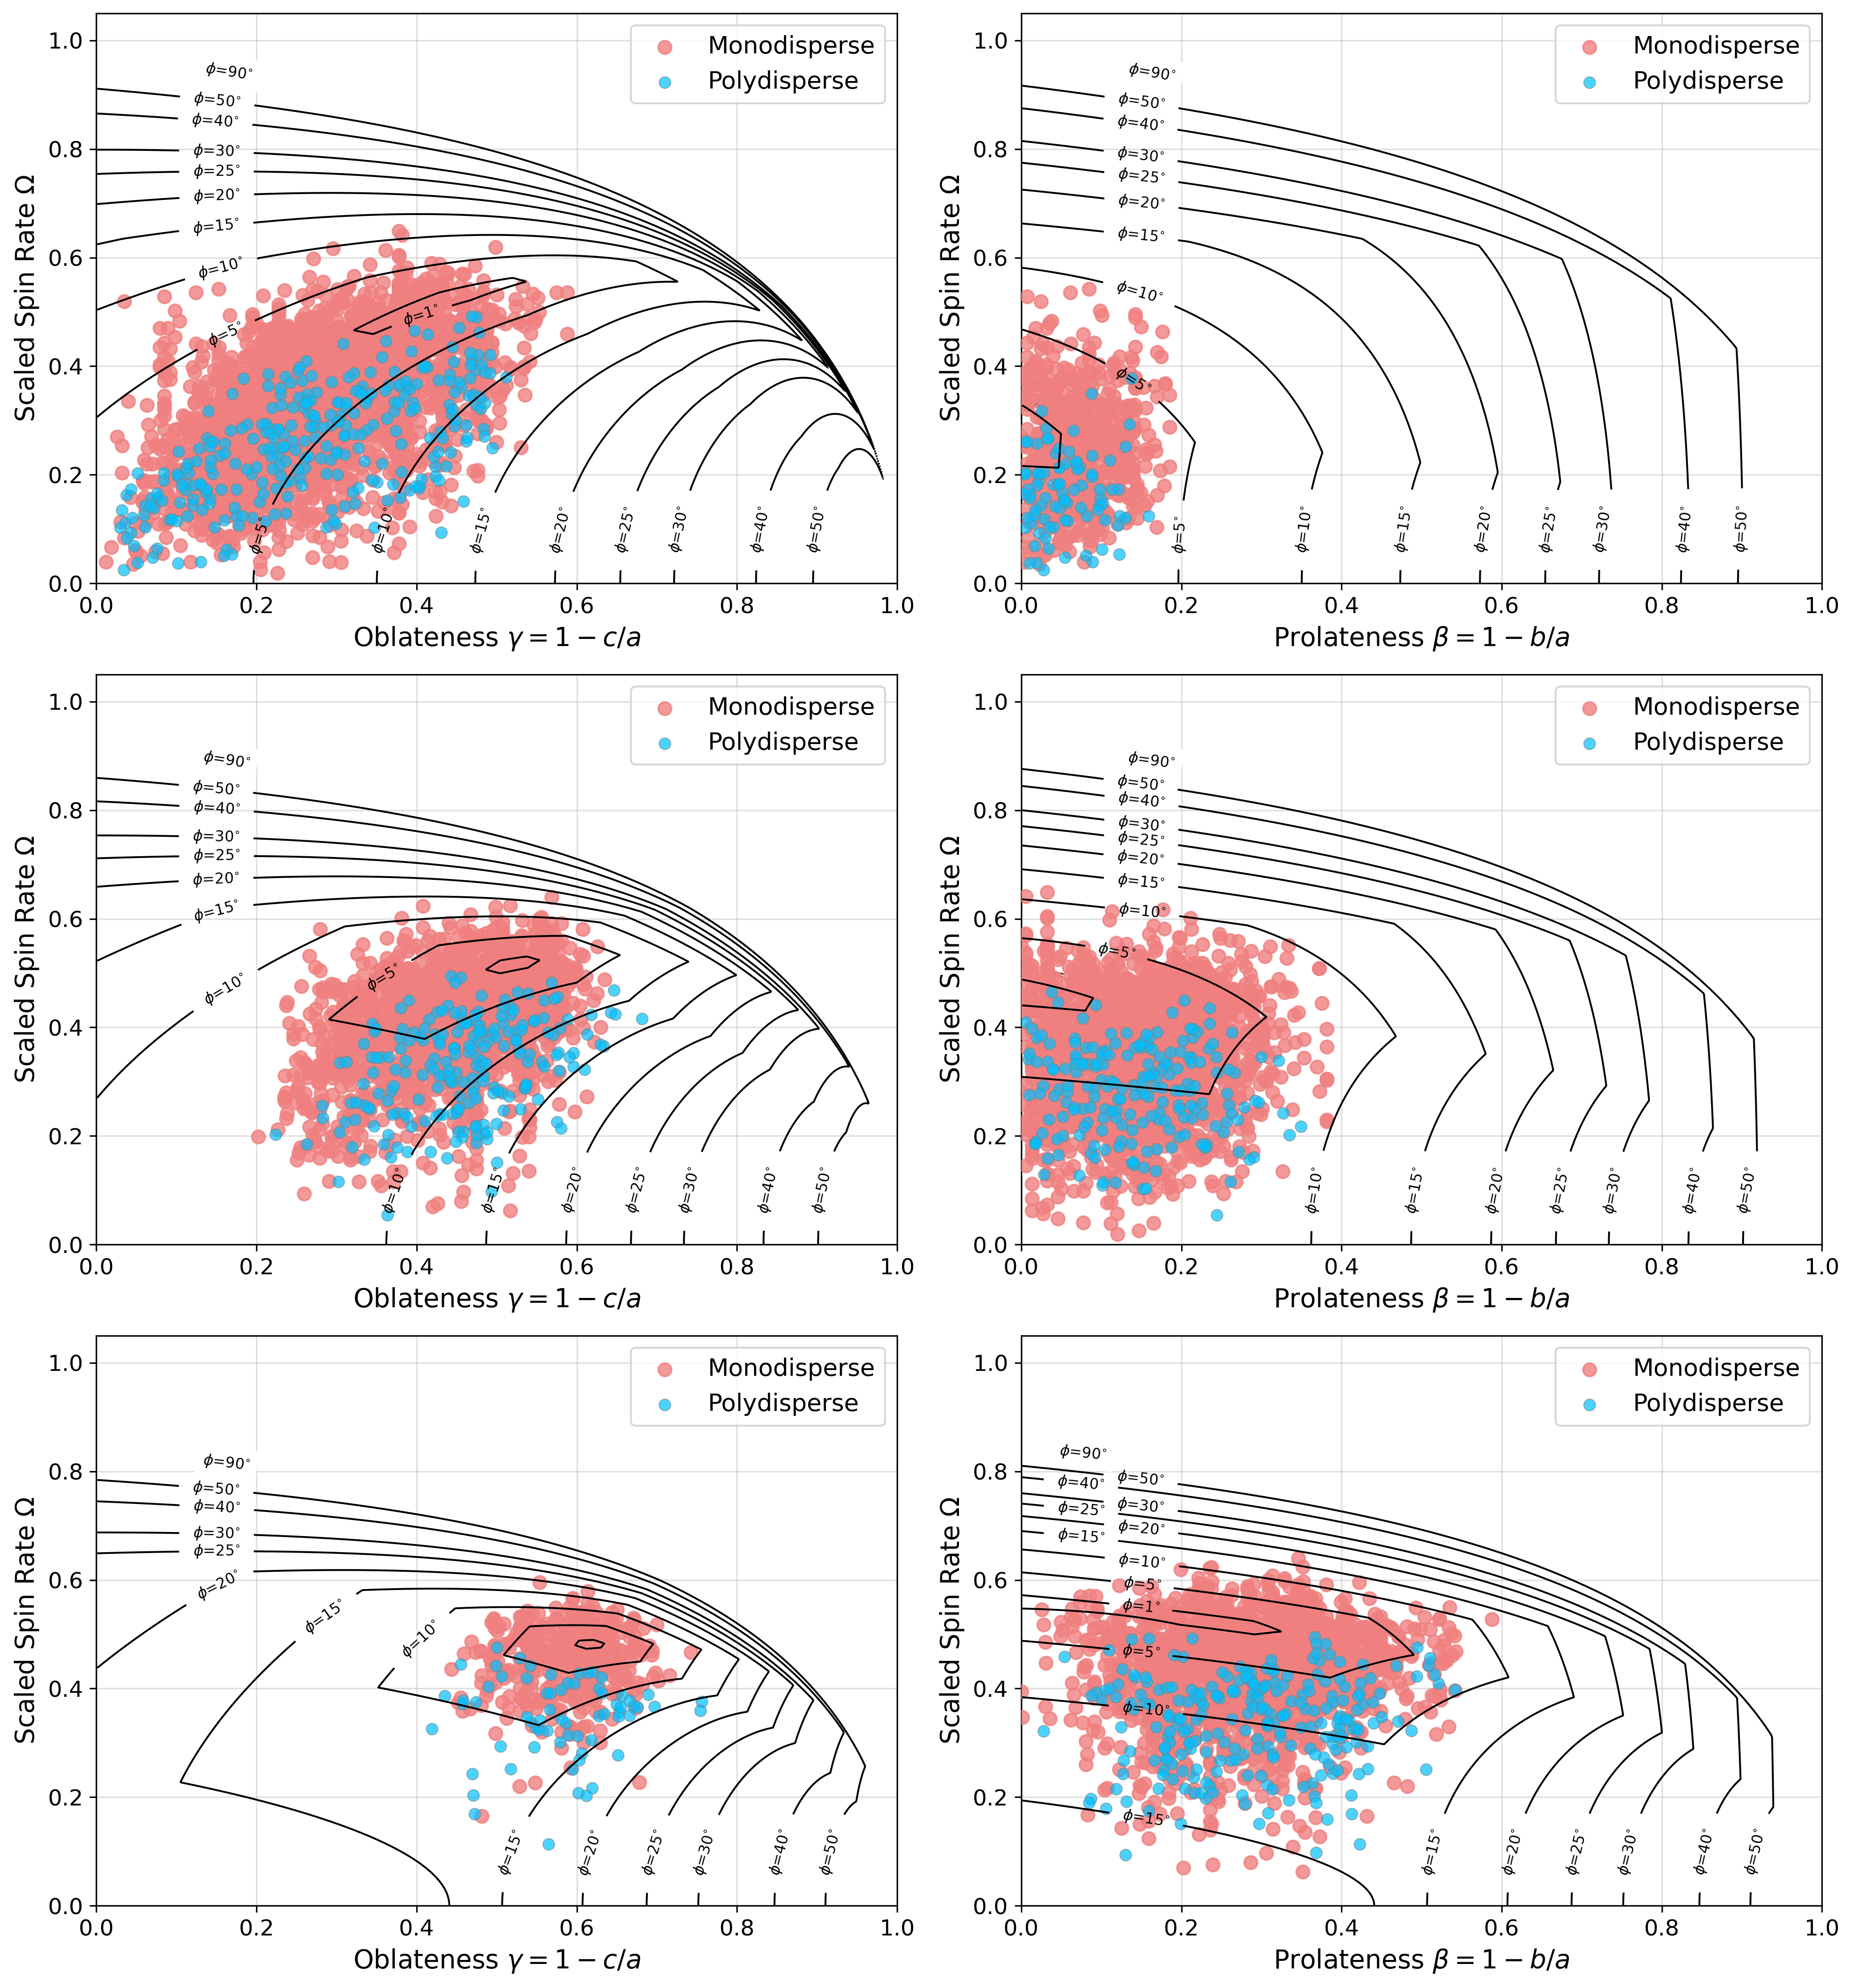
\includegraphics[width=\textwidth]{figures/scaled_spin_rate_vs_gamma_beta.png}
    \caption{Oblateness and prolateness vs.\ scaled spin rate for
    planetesimals with mass $M > 2^{-16} M_\odot$. Each point represents
    an individual planetesimal. The left panels show the scaled spin
    rate $\Omega = \omega/\sqrt{G\rho}$ as a function of oblateness
    $\gamma = 1 - c/a$, while the right panels show the same spin rate
    plotted against prolateness $\beta = 1 - b/a$. Pink points denote
    the monodisperse population and blue points the polydisperse
    population. Rows correspond to successive slices in the third
    (unshown) axis ratio: from top to bottom, $1 - b/a \approx 0.1,
    0.3, 0.5$ in the left panels and $1 - c/a \approx 0.1, 0.3, 0.5$ in
    the right panels, so that planetesimals become progressively more
    triaxial from top to bottom. Solid black contours indicate the
    internal friction angle $\phi$ (in degrees) required for a rotating
    triaxial body of the corresponding shape to remain stable at that
    spin rate, computed at the fixed third-axis ratio appropriate to
    each row.}
    \label{fig:oblateness_prolateness_vs_spin}
\end{figure*}

Figure~\ref{fig:oblateness_prolateness_vs_spin} shows the relation between planetesimal
shape and spin rate for objects with mass $M > 2^{-16} M_\odot$,
comparing the oblateness $\gamma = 1 - c/a$ (left column) and
prolateness $\beta = 1 - b/a$ (right column) against the scaled spin
rate $\Omega = \omega/\sqrt{G\rho}$. Because a triaxial body's shape is
described by two independent axis ratios, each row of the figure
restricts the plotted sample to a narrow range in the axis ratio not
shown on that panel, holding it approximately fixed at
$1 - b/a \approx 0.1$, $0.3$, and $0.5$ (top to bottom) in the left
column, and the analogous cut in $1-c/a$ in the right column. The
overplotted contours give the internal friction angle $\phi$ (in
degrees) required for a rotating body with that shape and spin to
remain mechanically stable, evaluated at the same fixed third-axis
ratio. Moving down the rows therefore traces the shape-spin relation
for increasingly triaxial (less axisymmetric) planetesimals.

Across all three rows, the monodisperse (pink) and polydisperse (blue)
populations occupy broadly overlapping regions of shape-spin space,
and both largely respect the same underlying stability boundary set by
the $\phi$ contours. A planetesimal lying below a given contour can
maintain its shape and spin rate with comparatively weak internal
cohesion, while a body lying above a contour would require an internal
friction angle exceeding that value to resist rotational disruption or
reshaping. That both suites populate the low-to-intermediate $\phi$
region of parameter space, and follow qualitatively similar
shape-spin trends across all three third-axis-ratio slices, indicates
that the basic mechanical limits on how fast a body of a given shape
can spin are set primarily by self-gravity and internal friction
rather than by the details of the accreting particle population. In
this respect, the shape-spin relation behaves as a shared outcome of
gravitational collapse, consistent with the similarly shared
spin-size trend identified in Section~4.1.1.

The clearest systematic departure from this shared behavior is that
the monodisperse population extends further toward higher oblateness
or prolateness and higher spin rates than its polydisperse
counterpart, which instead remains more tightly confined to
intermediate axis ratios and lower spin rates. This is most apparent
in the more triaxial slices (middle and bottom rows), where the
monodisperse population extends into regions requiring
$\phi \gtrsim 30$--$40^\circ$ for stability at the highest spin rates,
while the polydisperse population remains largely confined to
lower-$\phi$ contours across all three rows. Because the underlying
stability criterion is identical for both suites, this difference
cannot be attributed to the friction contours themselves, but instead
reflects how each particle population redistributes angular momentum
and dissipates energy during collapse: the presence of a size
distribution in the polydisperse runs appears to damp shape distortion
and spin-up more efficiently than in the monodisperse case, allowing
these bodies to settle into shapes and spins consistent with weaker
internal cohesion.

This divergence foreshadows the more substantial differences between
the two suites explored in Section~4.2, where particle-size diversity
is shown to systematically alter bulk density, rotation period, and
binary formation outcomes. Taken together, the shape-spin relation
established here suggests that while gravitational collapse imposes a
common mechanical framework on the resulting planetesimals, particle-
size diversity already begins to shape the finer details of that
outcome even before its effects become clearly visible in bulk
structural properties.

\subsection{Distinct Differences Between Monodisperse and Polydisperse Systems}\label{sec:different}
\subsubsection{Bulk density vs Normalized Mass}
\begin{figure*}
    \centering
    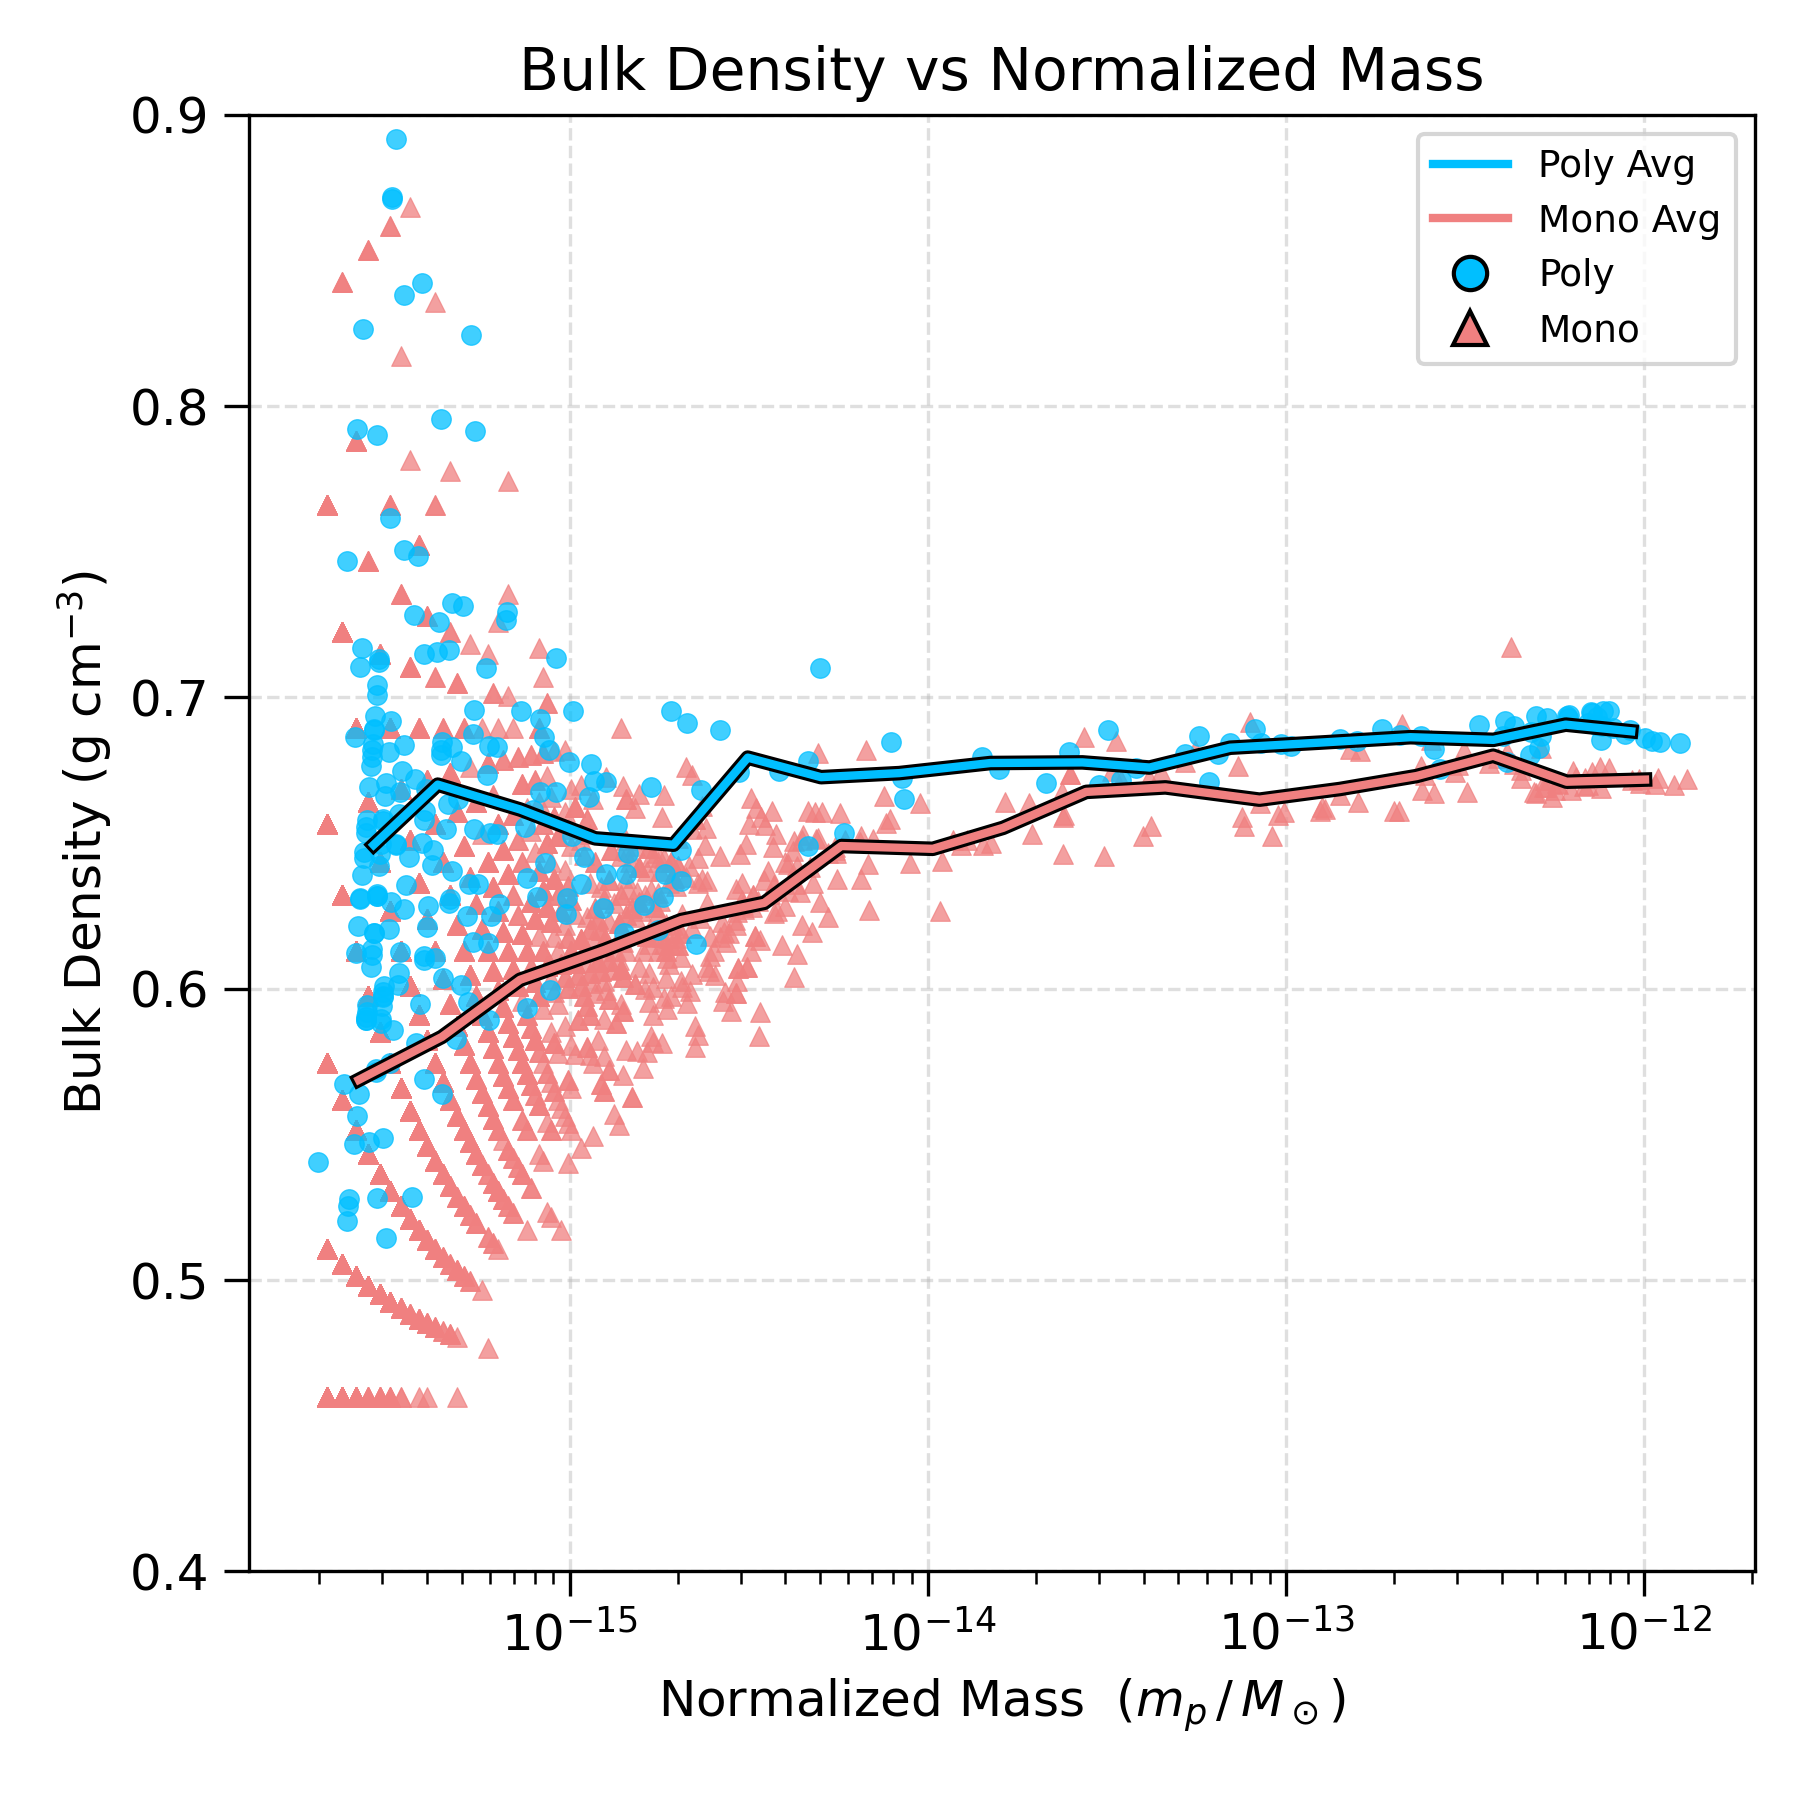
\includegraphics[width=\textwidth]{figures/bulk_density_scatter_normal.png}
    \caption{Bulk density as a function of normalized planetesimal mass
    ($m_p/M_\odot$) for the monodisperse (pink triangles) and
    polydisperse (blue circles) simulation suites. Solid lines show the
    corresponding moving-average trends for the polydisperse (blue) and
    monodisperse (pink) populations.}
    \label{fig:bulk_density_vs_mass}
\end{figure*}


Figure~\ref{fig:bulk_density_vs_mass} shows the relation between bulk density and normalized planetesimal mass for the monodisperse and polydisperse simulations. The x-axis gives the final mass of each object relative to the total cloud mass, while the y-axis gives its bulk density in g/cm$^3$. The scatter points show individual planetesimals, while the moving-average curves highlight the underlying trend. The marginal histograms provide additional context for how each population is distributed in both mass and density.

At low normalized masses, both populations show a wide spread in bulk density, indicating a range of internal structures and porosities. However, the distributions differ in detail. 
The monodisperse population extends more frequently to lower densities, while the polydisperse population is more concentrated toward intermediate and higher densities.
This reflects differences in how pore space is filled during collapse. 
In the monodisperse case, particles of similar size cannot efficiently fill the voids between one another, leaving larger pore spaces and producing more porous structures.
In contrast, the presence of smaller particles in the polydisperse simulations allows these voids to be partially filled, reducing porosity and leading to higher bulk densities in many of the smaller bodies. 

Rather than being a difference in ideal packing efficiency—since monodisperse systems can achieve ordered configurations such as hexagonal close packing—the key distinction here arises from the dynamical collapse process.
The irregular and time-dependent assembly of particles prevents perfect ordering, and the availability of multiple particle sizes in the polydisperse case allows for more effective filling of gaps during gravitational aggregation.

As normalized mass increases, the spread in densities decreases and the moving-average curves for both populations converge.
Beyond \(m_p/M_{\text{cloud}} \sim 10^{-12}\), both systems approach bulk densities of about \(0.67\)–\(0.69\ \mathrm{g\,cm^{-3}}\). 
This convergence suggests that as objects grow larger, self-gravity becomes the dominant factor controlling internal structure. 
The increasing gravitational compression reduces porosity and drives both monodisperse and polydisperse bodies toward similar equilibrium densities.

Overall, the figure shows that particle-size diversity plays a significant role in setting the porosity and internal structure of smaller planetesimals, but this dependence weakens as mass increases.
Larger bodies undergo sufficient gravitational compaction that their final bulk densities become largely independent of their initial particle size distribution, indicating that the collapse process erases much of the memory of the initial conditions at higher masses.

\subsubsection{Binary Formation Efficiency and Frequency}

\begin{figure*}
    \centering
    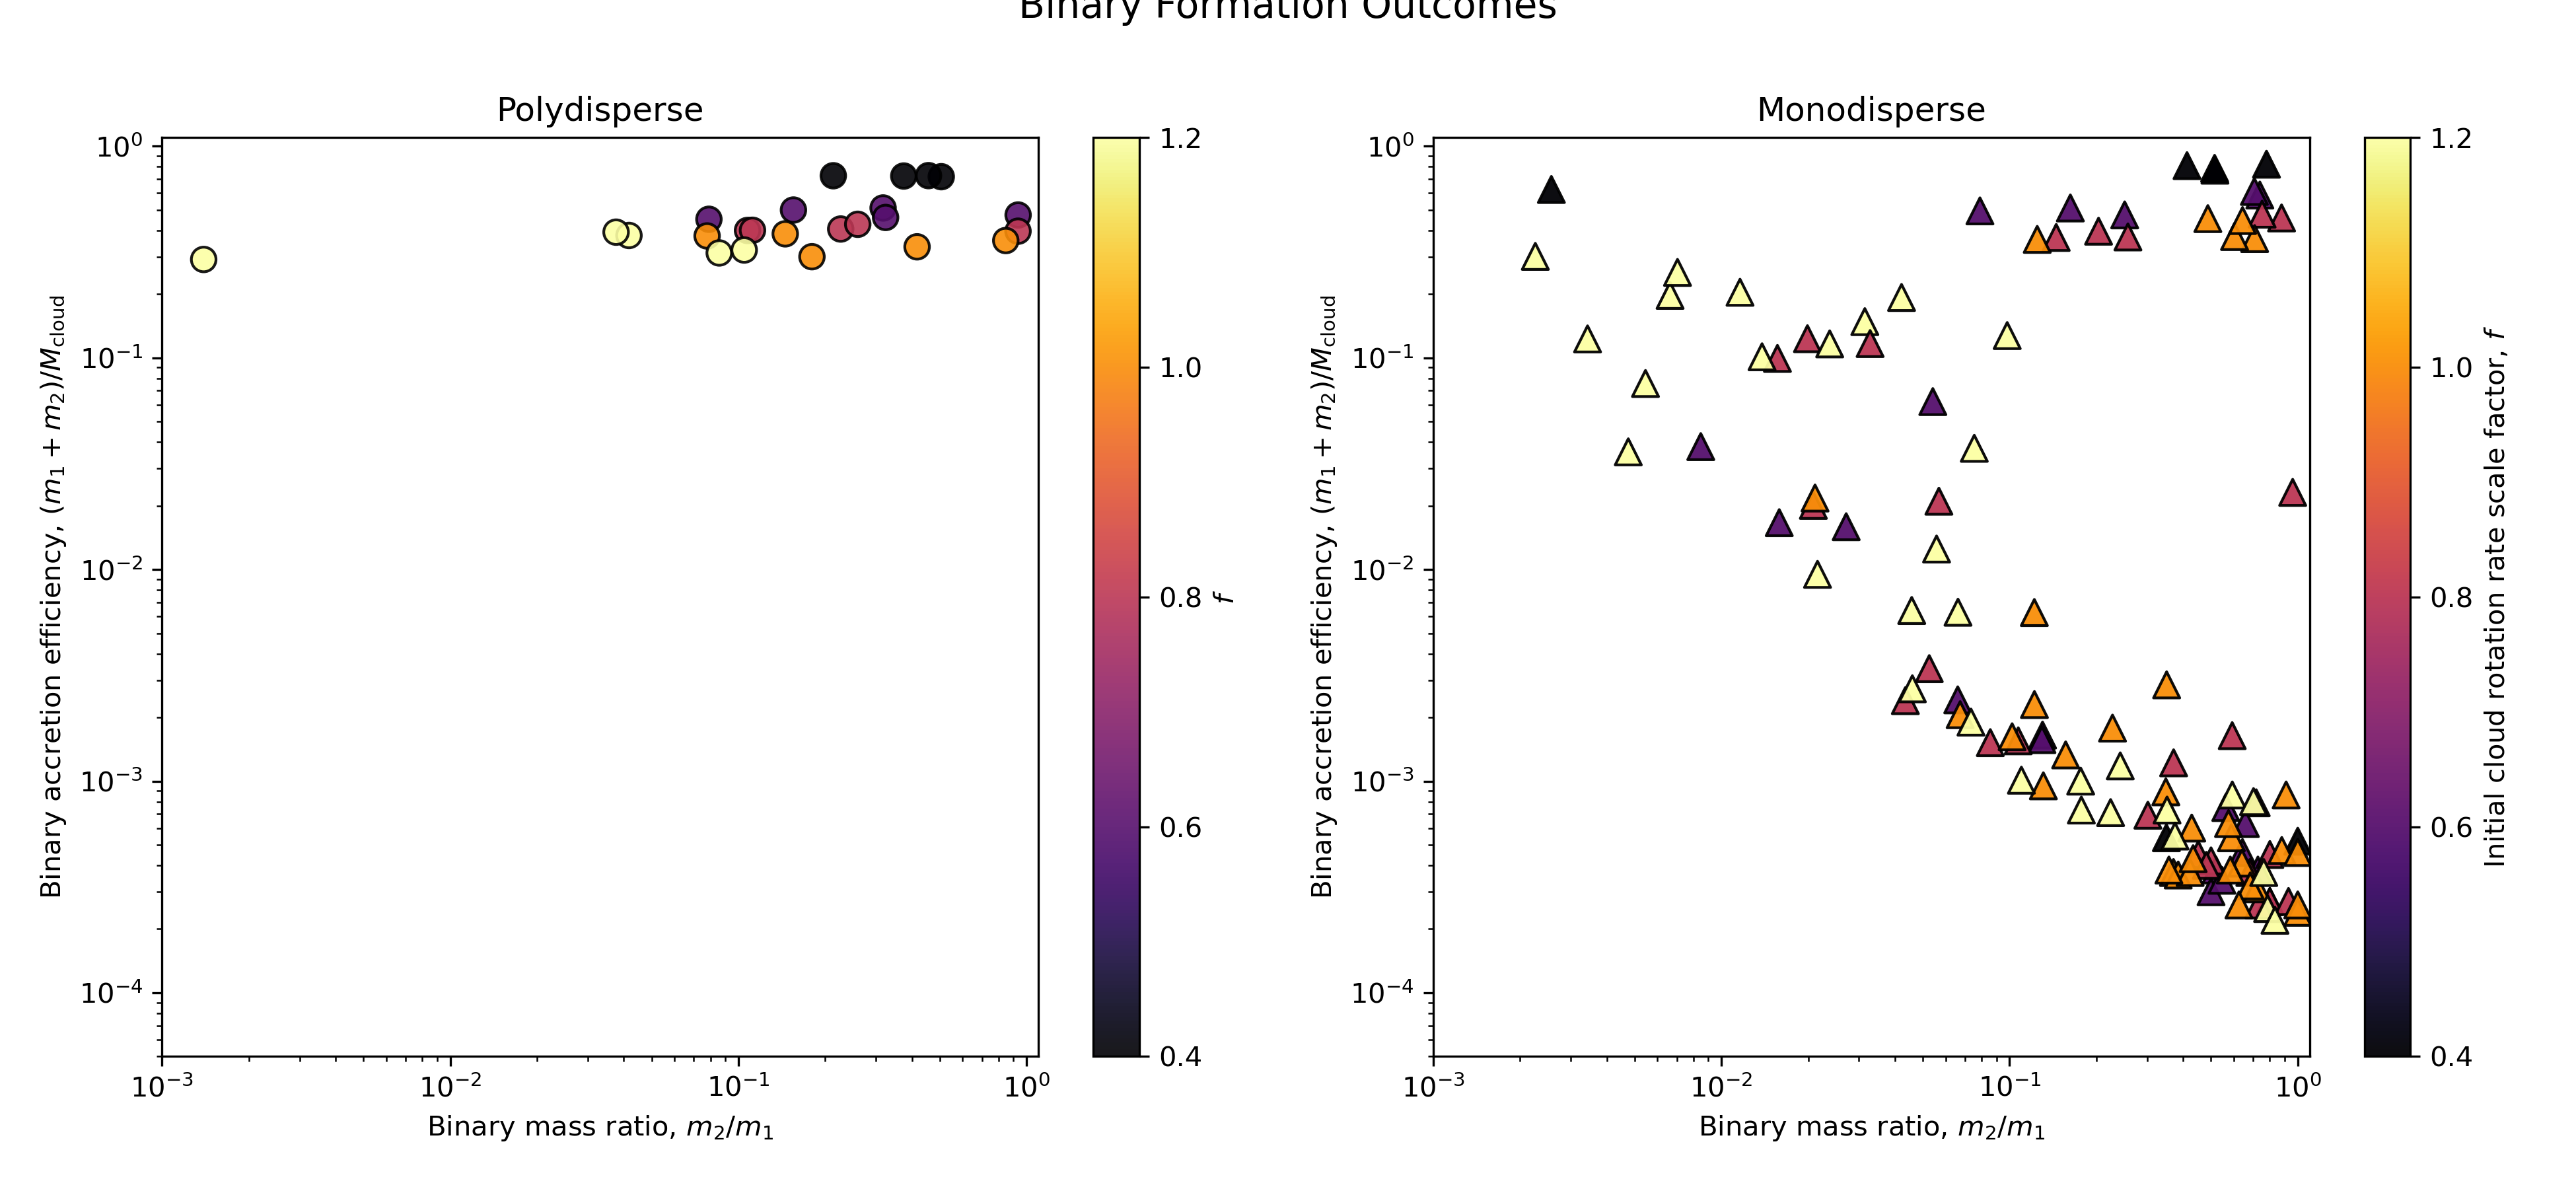
\includegraphics[width=\textwidth]{figures/binary_side_by_side.png}
    \caption{Binary formation outcomes in polydisperse (left, circles)
    and monodisperse (right, triangles) gravitational collapse
    simulations. In both panels, the horizontal axis shows the binary
    mass ratio, $m_2/m_1$, and the vertical axis shows the binary
    accretion efficiency, $(m_1+m_2)/M_{\rm cloud}$. Points are
    colored by the initial cloud rotation rate scale factor $f$. Both
    component masses are restricted to $m_1, m_2 \geq 2\times10^{-16}\,
    M_{\rm cloud}$ in each panel.}
    \label{fig:binary_formation_comparison}
\end{figure*}

Figure~\ref{fig:binary_formation_comparison} compares binary formation
outcomes between the polydisperse and monodisperse simulation suites,
applying the same minimum component mass,
$m_1, m_2 \geq 2\times10^{-16}\,M_{\rm cloud}$, to both. The horizontal
axis gives the \textit{binary mass ratio}, $m_2/m_1$, where $m_1$ and
$m_2$ are the primary and secondary component masses, with
$m_2/m_1 = 1$ corresponding to an equal-mass binary. The vertical axis
gives the \textit{binary accretion efficiency},
$(m_1+m_2)/M_{\rm cloud}$, the fraction of the total initial cloud
mass captured into the binary. Points are colored by the initial cloud
rotation rate scale factor $f$, with darker colors corresponding to
slower rotation and lighter colors to more rapid rotation.

The two populations show markedly different structure. The
\textbf{polydisperse} suite (left) produces comparatively few binaries,
and these separate into two distinct groups rather than following a
single continuous trend: the majority cluster at moderate-to-high mass
ratios ($m_2/m_1 \gtrsim 0.03$) and high accretion efficiency
($(m_1+m_2)/M_{\rm cloud} \sim 0.2$--$1$), while a small number of
outliers at low mass ratio ($m_2/m_1 \sim 10^{-3}$--$10^{-2}$) fall to
much lower efficiency ($\lesssim 10^{-2}$). Within the dominant
high-efficiency group, efficiency shows little systematic dependence
on mass ratio, indicating that once a polydisperse cloud forms an
efficient binary, that efficiency is largely insensitive to how
evenly the mass is split between the two components.

The \textbf{monodisperse} suite (right), in contrast, produces many
more binaries that populate a smooth, continuous trend spanning the
entire range of mass ratios. Accretion efficiency declines steadily
and monotonically as $m_2/m_1$ decreases, falling from
$(m_1+m_2)/M_{\rm cloud} \sim 1$ at $m_2/m_1 \sim 1$ down to
$\sim 10^{-4}$ at $m_2/m_1 \sim 10^{-3}$, with no comparable
bifurcation into distinct efficiency groups. Faster-rotating clouds
(lighter colors) are concentrated toward the low-efficiency,
low-mass-ratio end of this trend, while slower-rotating clouds
(darker colors) populate the efficient, near-equal-mass end, indicating
that rotation more directly controls binary outcome in the
monodisperse case than in the polydisperse one.

Taken together, these results show that particle-size diversity
strongly influences both the frequency and character of binary
formation. Polydisperse clouds form fewer binaries, but those that do
form tend to capture a large, relatively mass-ratio-independent
fraction of the cloud mass -- consistent with enhanced angular
momentum transport during collapse smoothing out the accretion
process. Monodisperse clouds instead produce a much larger number of
binaries whose efficiency is tightly coupled to both mass ratio and
rotation rate, reflecting less efficient, more strongly
rotation-dependent accretion under uniform particle conditions.

\begin{figure}[htbp]
    \centering
    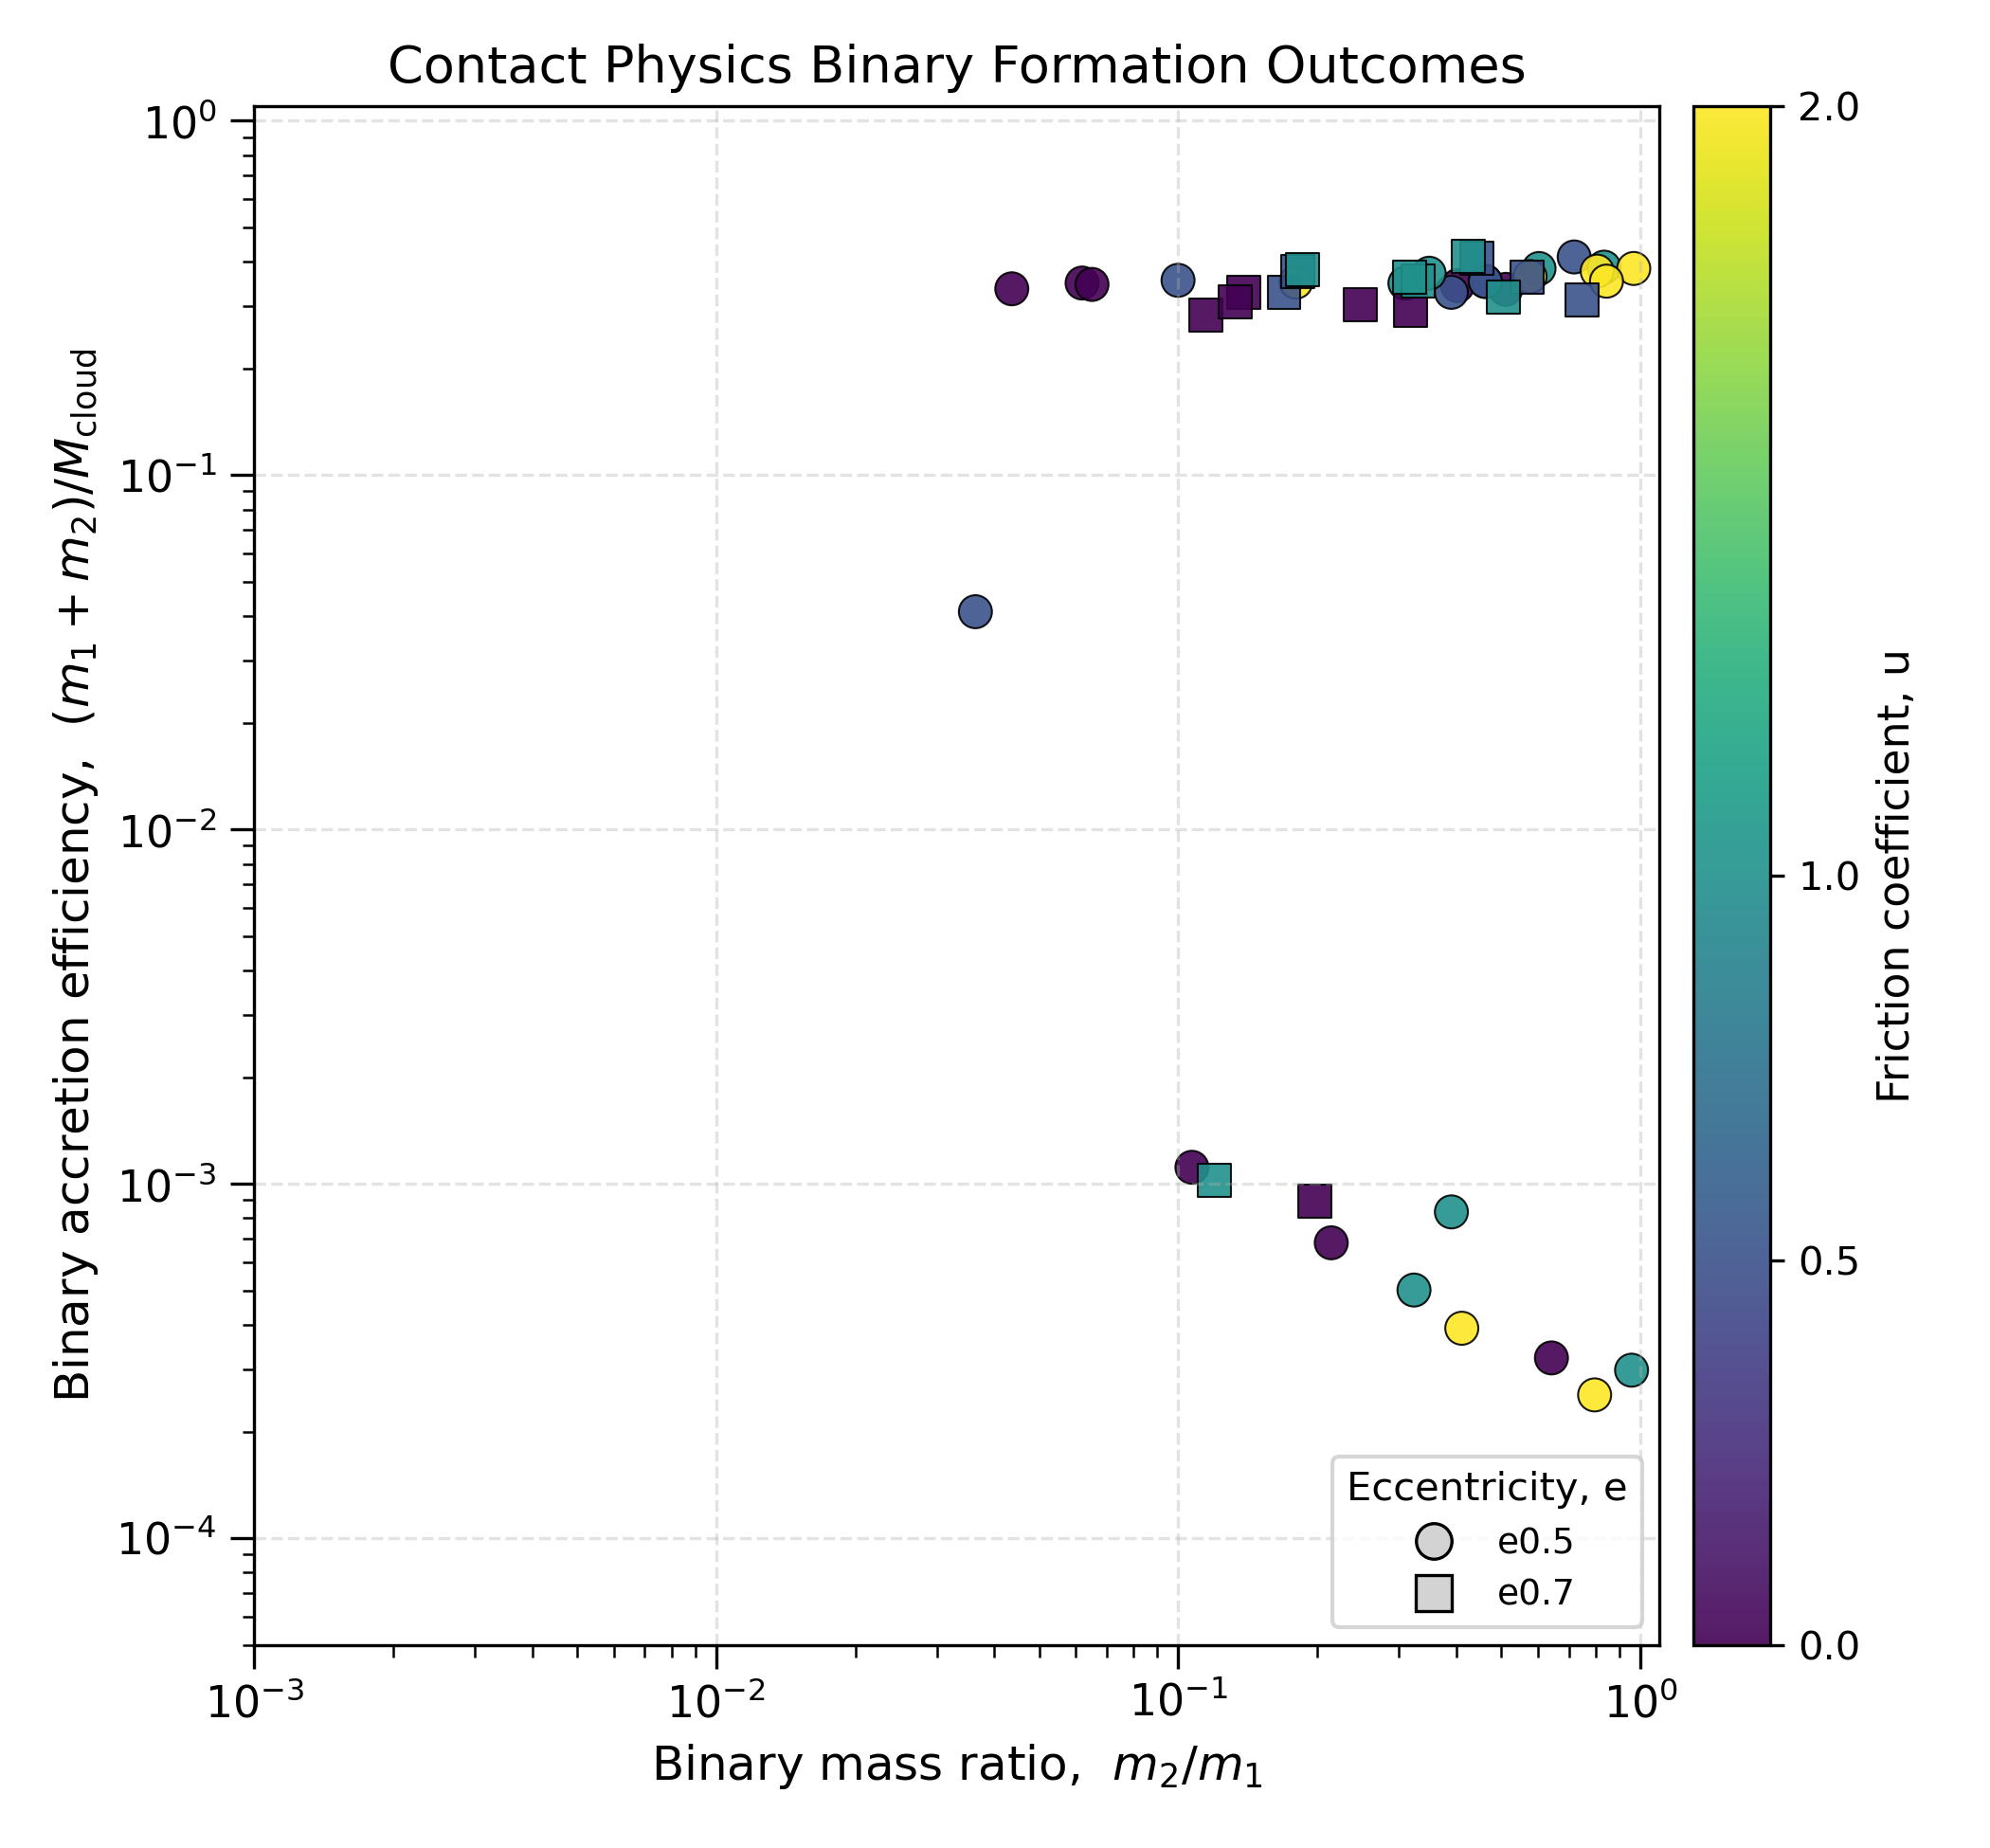
\includegraphics[width=\columnwidth]{figures/binary_contact_physics.png}
    \caption{Contact-physics binary formation outcomes: binary
    accretion efficiency $(m_1+m_2)/M_{\rm cloud}$ versus binary mass
    ratio $m_2/m_1$ for the polydisperse simulations that include
    interparticle friction, with the same minimum component mass,
    $m_1, m_2 \geq 2\times10^{-16}\,M_{\rm cloud}$, applied. Points are
    colored by the friction coefficient $u$; circles denote systems
    with eccentricity $e = 0.5$ and squares denote $e = 0.7$.}
    \label{fig:binary_contact_physics}
\end{figure}

Figure~\ref{fig:binary_contact_physics} shows the same mass-ratio
vs.\ accretion-efficiency relation for the polydisperse simulations
that additionally include interparticle friction. As in the
frictionless polydisperse case, these systems separate into two
distinct efficiency regimes rather than following the smooth,
continuous trend seen in the monodisperse suite: a cluster of binaries
with $m_2/m_1 \gtrsim 0.1$ achieving efficiencies of
$(m_1+m_2)/M_{\rm cloud} \sim 0.3$--$0.4$, comparable to the
frictionless polydisperse case, and a smaller group at similarly
moderate-to-high mass ratios that instead settle at markedly lower
efficiencies of $(m_1+m_2)/M_{\rm cloud} \sim 10^{-4}$--$10^{-3}$.
There is no clear trend of accretion efficiency with the friction
coefficient $u$ itself, suggesting that friction primarily governs
\emph{whether} a collapse produces an efficient, massive binary at
all, rather than smoothly tuning the efficiency of binaries that do
form. This bimodal, mass-ratio-independent character persists from the
frictionless to the friction-included polydisperse case, in contrast
to the continuous, mass-ratio-dependent trend that instead
characterizes the monodisperse suite in
Figure~\ref{fig:binary_formation_comparison}.

\begin{figure}[htbp]
    \centering
    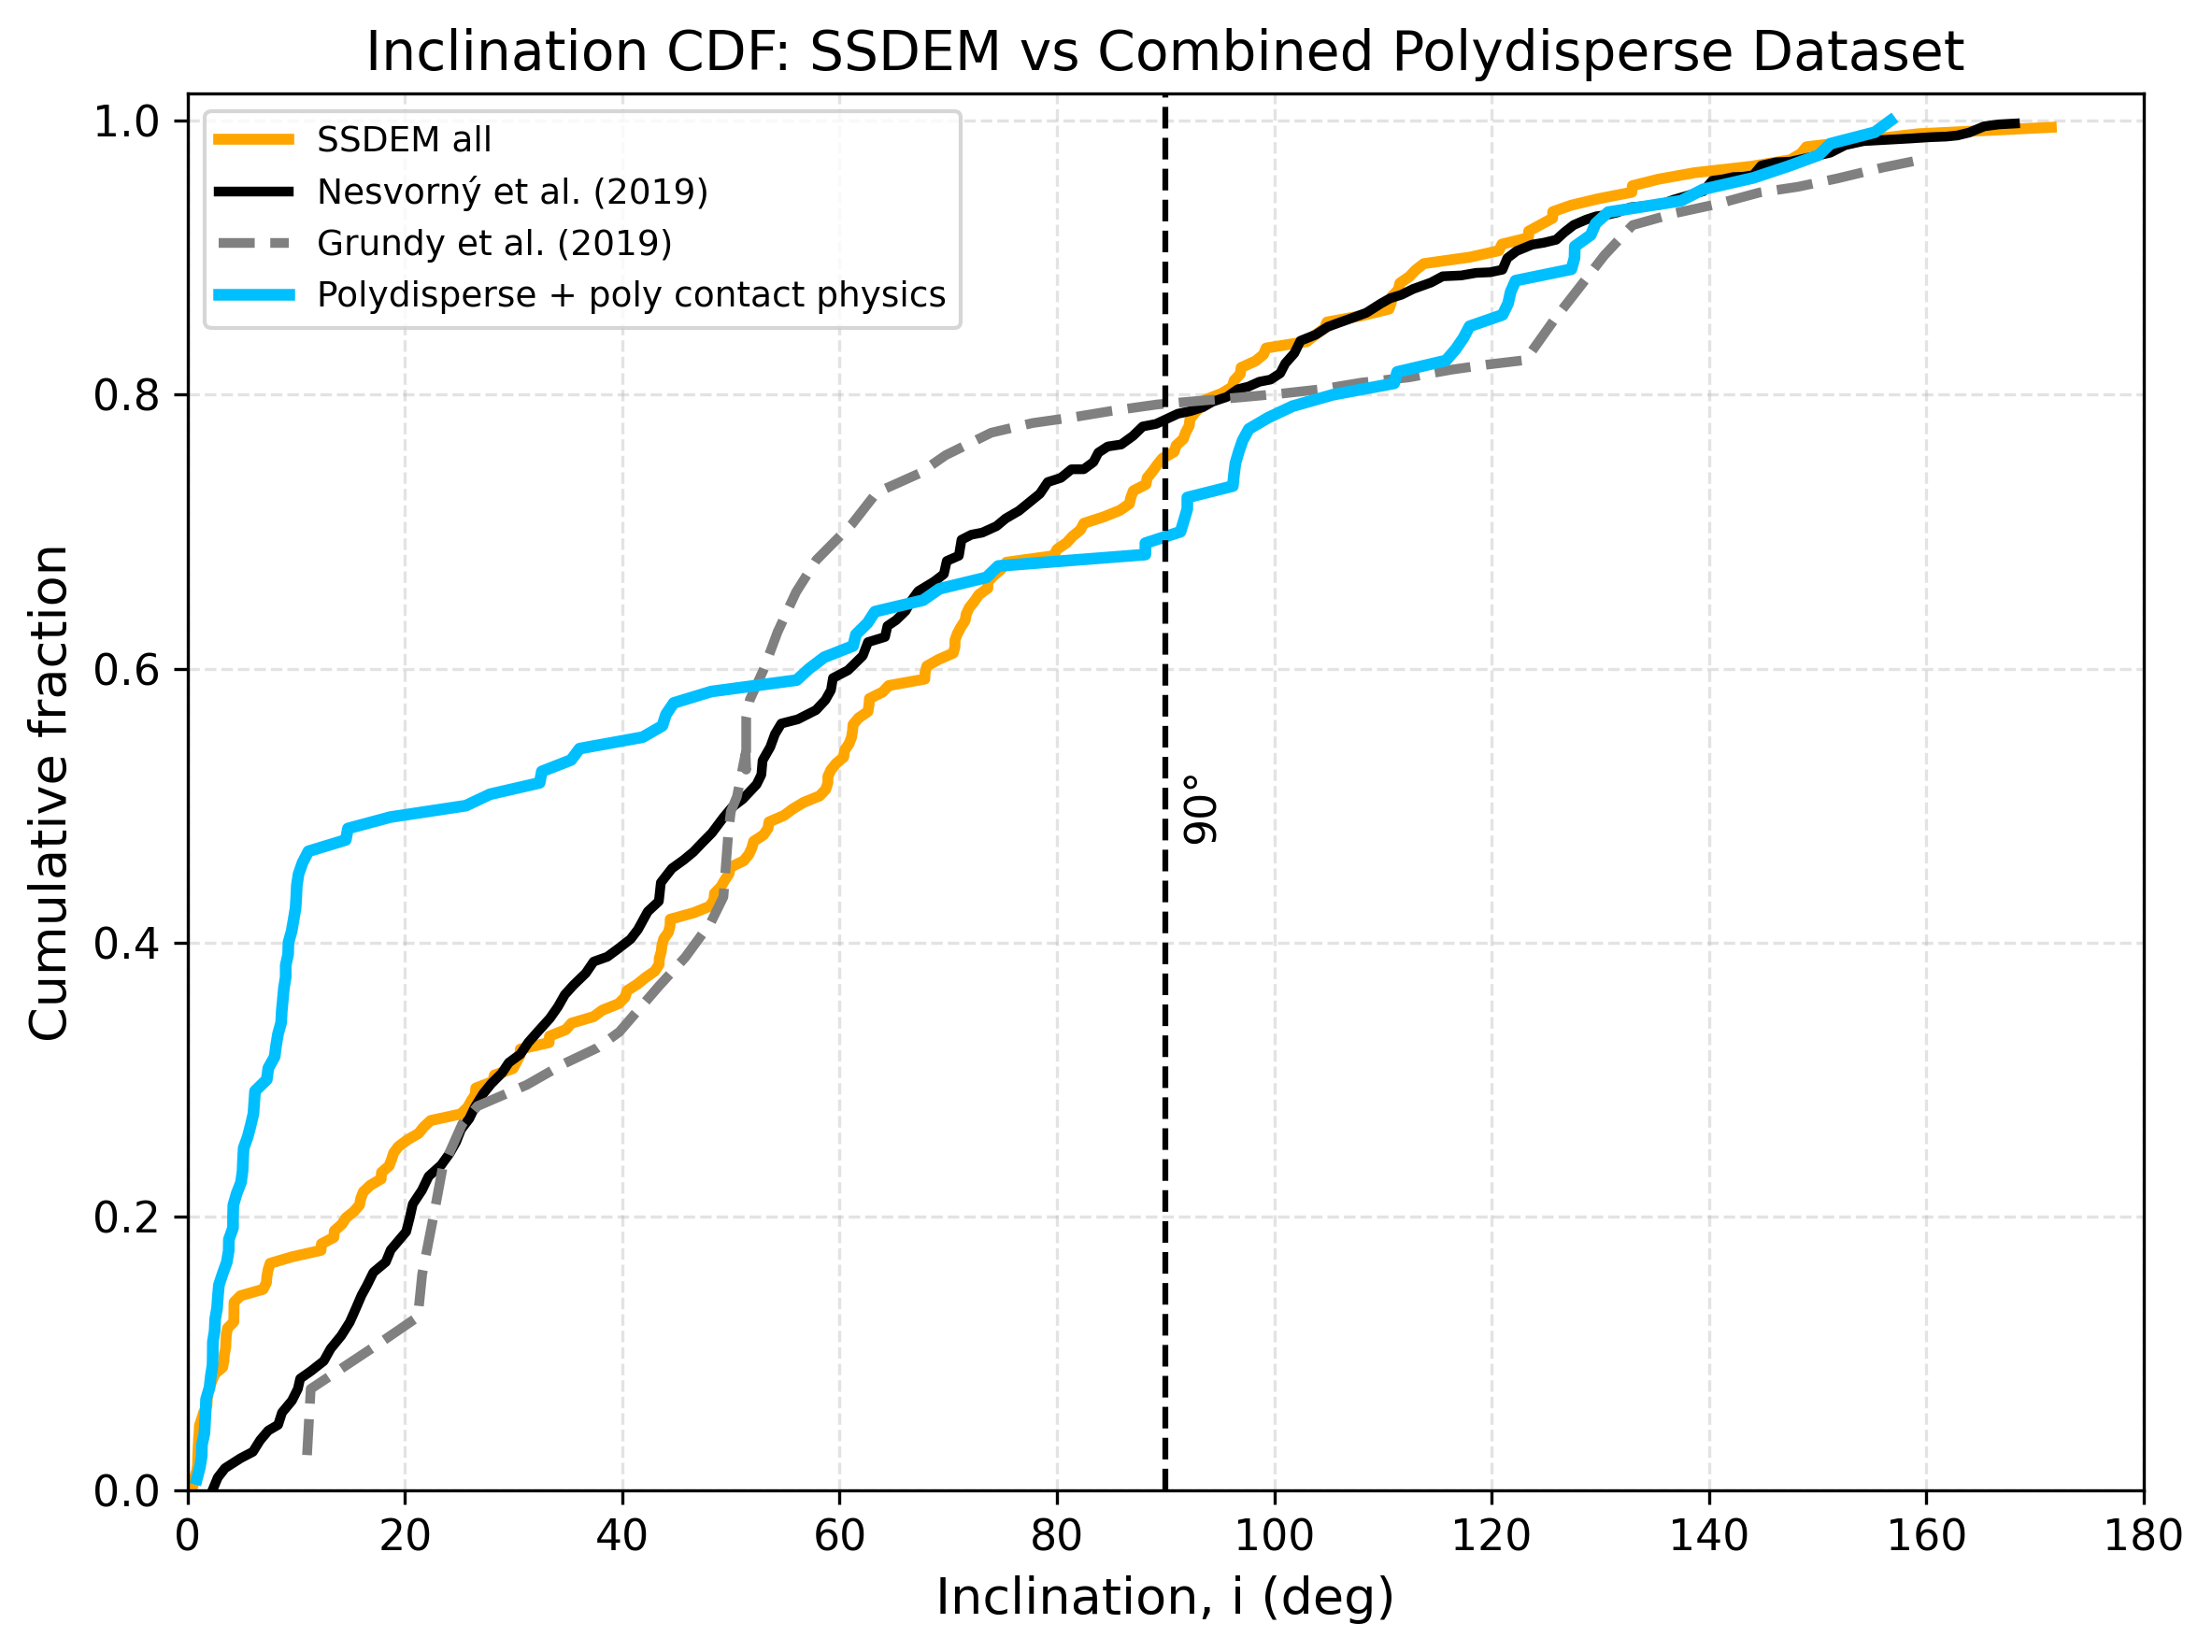
\includegraphics[width=0.8\columnwidth]{figures/inc_cdf_ssdem_nesvorny_grundy_combined_poly.png}
    \caption{Cumulative fraction of binary planetesimals with
    inclination less than or equal to the value on the abscissa.
    Results from our polydisperse SSDEM simulations are shown in
    orange (full polydisperse binary dataset) and blue (polydisperse
    simulations including contact-physics friction), and are compared
    to the streaming-instability model of Nesvorn\'y et al. (2019,
    black) and the observed trans-Neptunian binaries of Grundy et al.
    (2019, gray dashed). The vertical dashed line at $90^\circ$
    indicates the separation between prograde and retrograde orbits.}
    \label{fig:inclination-cdf}
\end{figure}

Having established how efficiently binaries form and how their masses
are distributed between components, we next examine the orbital
orientation of these systems. Figure~\ref{fig:inclination-cdf}
compares the cumulative distribution of inclinations for binary
planetesimals formed in our polydisperse SSDEM simulations to the
streaming-instability model of Nesvorn\'y et al. (2019) and the
observed population of trans-Neptunian binaries from Grundy et al.
(2019). The orange curve, representing the full polydisperse binary
dataset, tracks the Nesvorn\'y et al. (2019) distribution closely
across most of the inclination range, and both curves cross the
$90^\circ$ line at a cumulative fraction of $\approx 0.8$, indicating
that roughly $80\%$ of binaries in both datasets are prograde. The
Grundy et al. (2019) observational sample rises more steeply at
low-to-intermediate inclinations ($i \lesssim 60^\circ$) before
flattening out near $i \sim 90$--$130^\circ$, reflecting a real
population that is somewhat more concentrated toward low-inclination,
prograde orbits than either simulated dataset.

The polydisperse simulations including contact-physics friction
(blue) depart most noticeably from the other three curves at low
inclination: this population reaches a cumulative fraction of
$\approx 0.5$ by $i \sim 10^\circ$, far earlier than the orange SSDEM
curve, the Nesvorn\'y et al. (2019) model, or the observed Grundy et
al. (2019) sample, indicating that interparticle friction produces a
substantially larger fraction of low-inclination, nearly coplanar
binaries than either the frictionless polydisperse simulations or the
observed trans-Neptunian population. Beyond $i \sim 50^\circ$,
however, the friction-included curve flattens and largely converges
with the frictionless orange curve, crossing the $90^\circ$ line at a
similar cumulative fraction of $\approx 0.8$. This suggests that
internal friction primarily suppresses the formation of highly
inclined binaries at low inclination while leaving the overall
prograde/retrograde balance of the population largely unchanged --
consistent with the bimodal, friction-dependent efficiency outcomes
already seen in Figure~\ref{fig:binary_contact_physics}.

\begin{figure*}
    \centering
    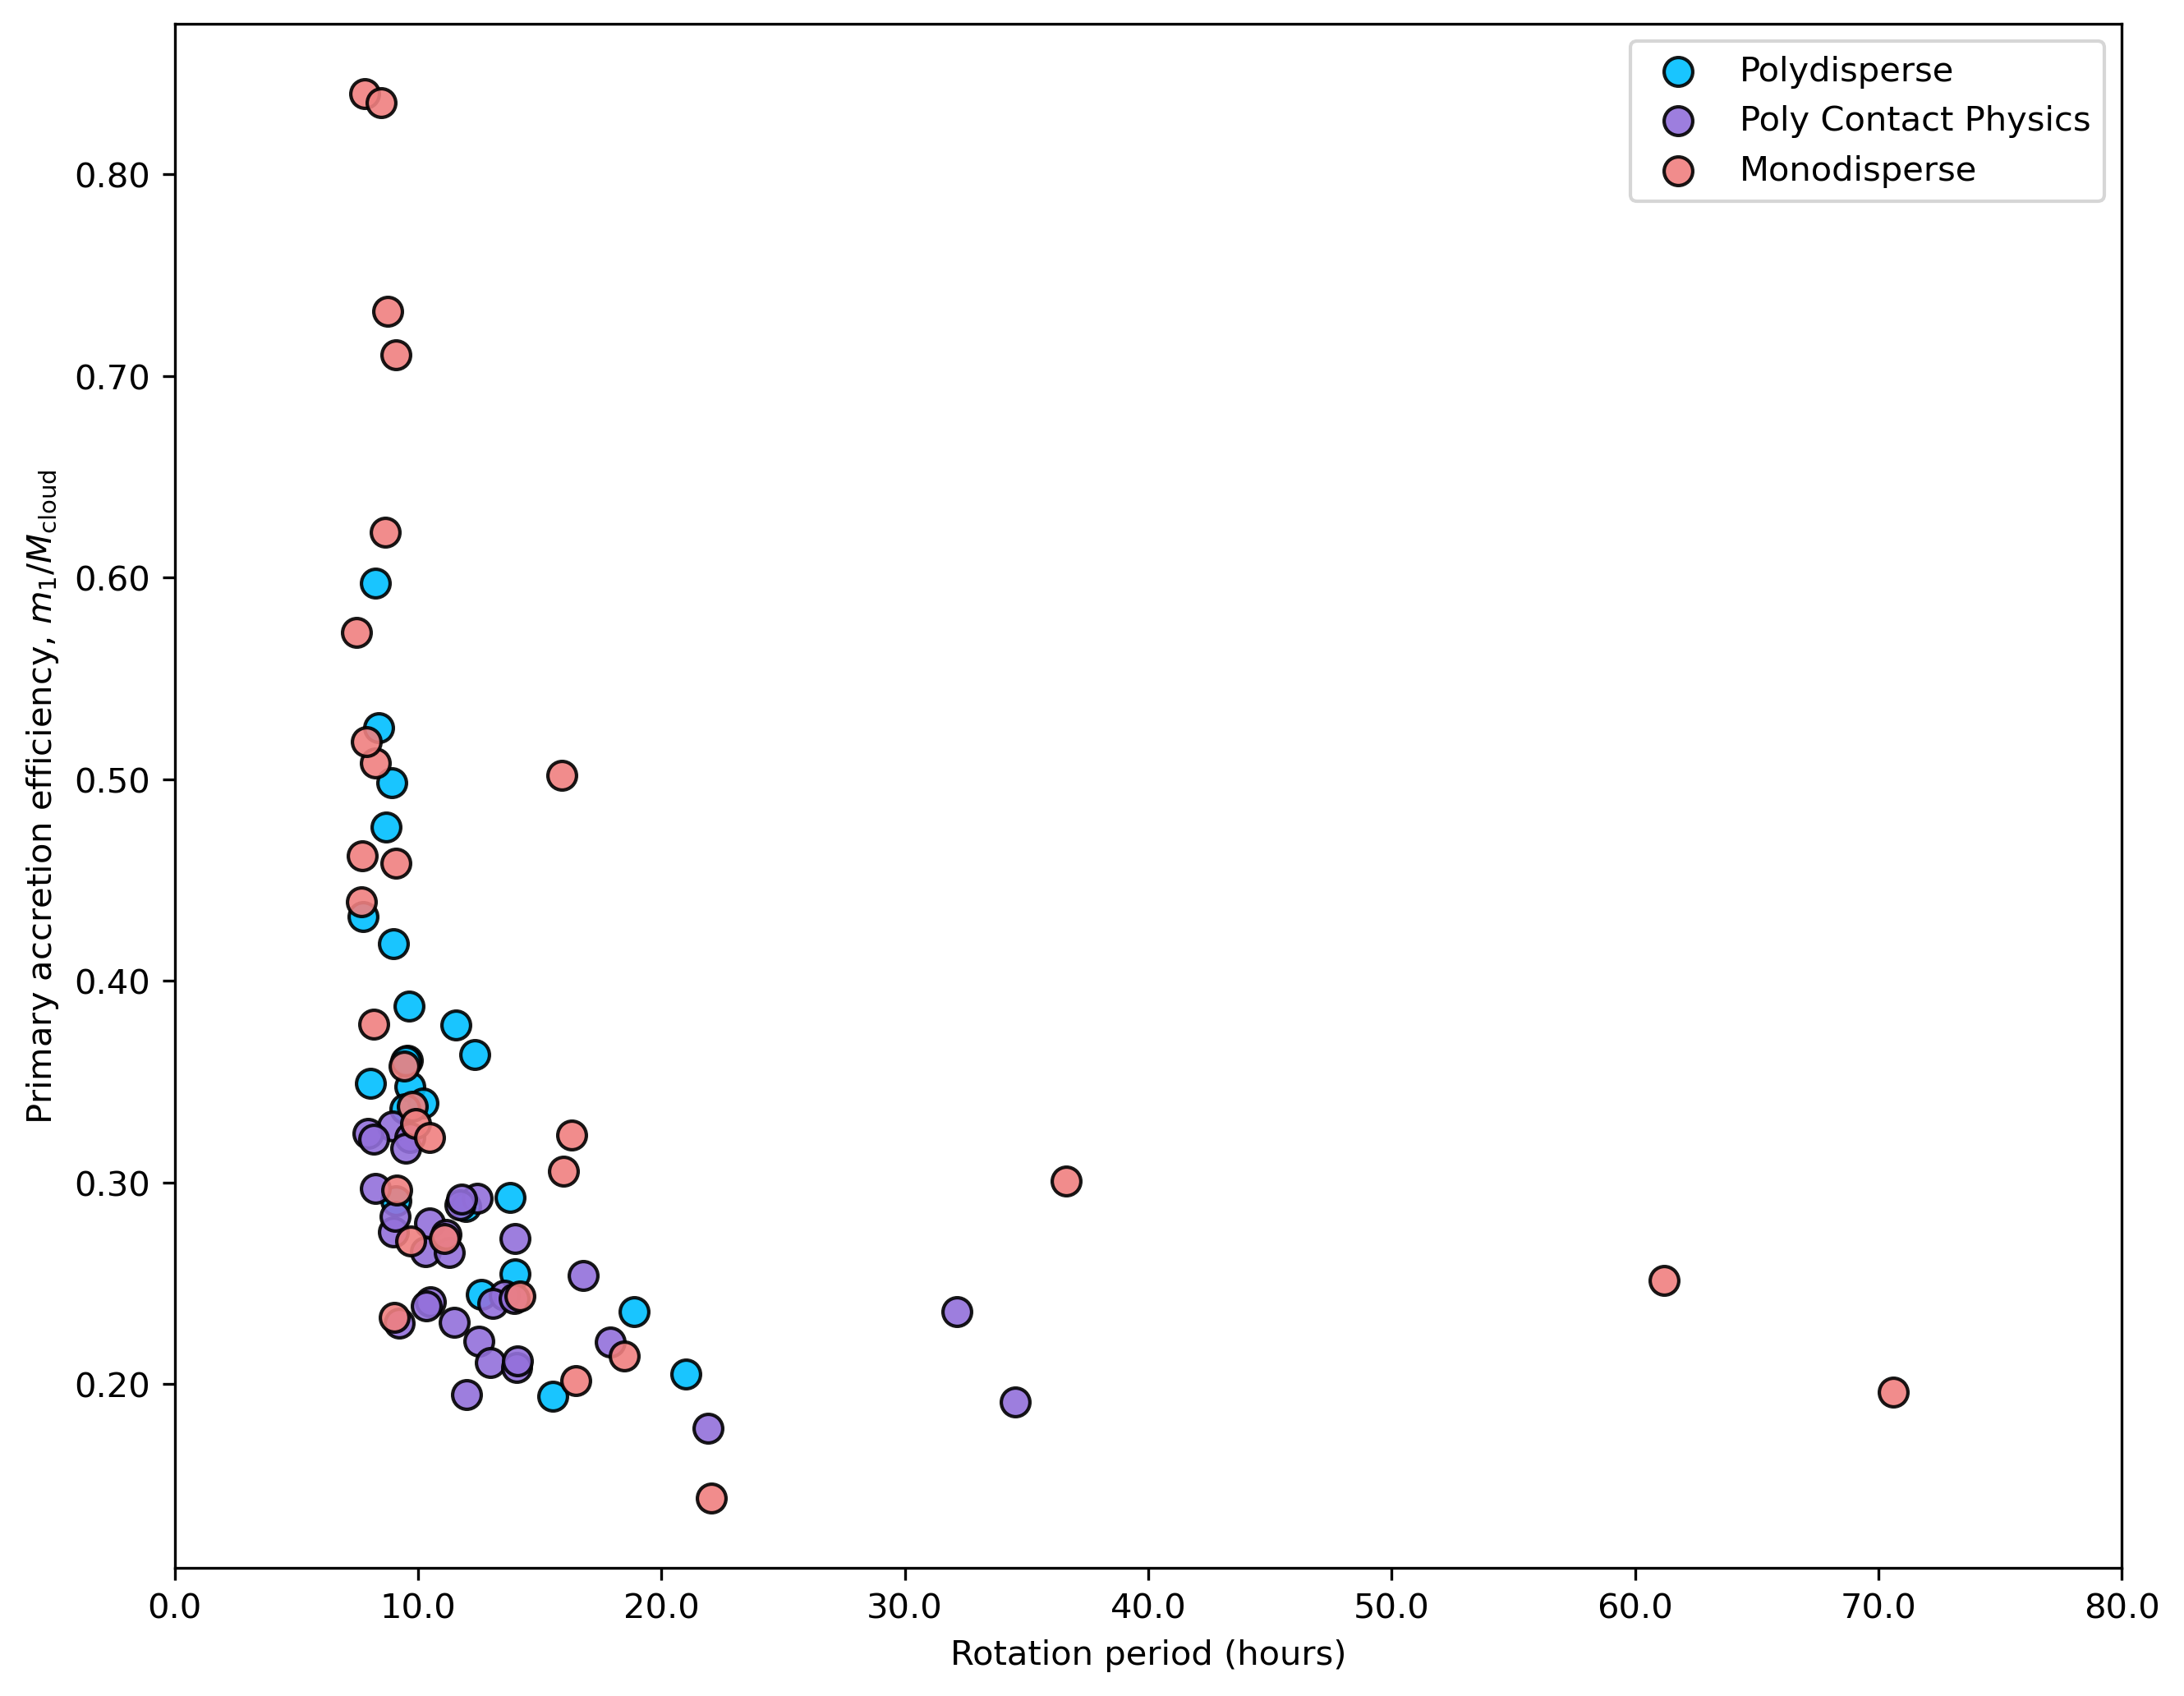
\includegraphics[width=\textwidth]{figures/most_massive_rotation_vs_accretion.png}
    \caption{Primary accretion efficiency, $m_1/M_{\rm cloud}$, as a
    function of rotation period (hours) for the most massive
    planetesimal formed in each simulation. Blue points denote the
    polydisperse suite, purple points denote polydisperse simulations
    including contact-physics friction, and pink points denote the
    monodisperse suite.}
    \label{fig:rotation-vs-accretion}
\end{figure*}

Because a large fraction of the bound mass in many of these
simulations resides in the most massive body -- whether or not it has
a bound companion -- it is useful to examine how efficiently that
single body accretes as a function of its final spin.
Figure~\ref{fig:rotation-vs-accretion} shows the accretion efficiency
of the most massive planetesimal formed in each simulation,
$m_1/M_{\rm cloud}$, as a function of its rotation period. Across all
three suites, the highest accretion efficiencies
($m_1/M_{\rm cloud} \gtrsim 0.5$) are achieved almost exclusively at
short rotation periods ($\lesssim 10$ hours), and efficiency falls off
steeply as the rotation period increases. The monodisperse population
reaches the highest efficiencies overall, with several simulations
exceeding $m_1/M_{\rm cloud} \approx 0.7$--$0.85$ at periods below
$10$ hours. The polydisperse population (without contact-physics
friction) follows a similar trend but does not reach quite as high an
efficiency at short periods, while still populating the same
short-period, high-efficiency region as the monodisperse suite. This
indicates that, for the most massive body formed in a given collapse,
rapid final rotation is closely associated with efficient mass
capture, largely independent of the particle-size distribution.

The polydisperse simulations that include contact-physics friction
depart most clearly from this pattern. These points are systematically
confined to a narrower range of rotation periods ($\sim 10$--$35$
hours) and to lower accretion efficiencies ($m_1/M_{\rm cloud}
\lesssim 0.3$), with no points reaching the high-efficiency,
short-period regime populated by the other two suites. This suggests
that interparticle friction suppresses the runaway accretion that
produces the most efficient primaries in the frictionless cases,
instead redistributing angular momentum and mass more evenly across
the collapsing cloud -- again mirroring the systematic suppression of
high-efficiency binaries seen for the same suite in
Figure~\ref{fig:binary_contact_physics}. At the longest rotation
periods ($\gtrsim 40$ hours), only monodisperse simulations are
present, extending out to periods of $\sim 60$--$70$ hours at low
efficiency ($m_1/M_{\rm cloud} \approx 0.2$--$0.3$); the absence of
polydisperse points in this regime may indicate that polydisperse
collapses more consistently avoid producing such slowly rotating,
inefficient primaries, though with the limited number of points here
this should be treated as suggestive rather than conclusive.

\begin{figure}[htbp]
    \centering
    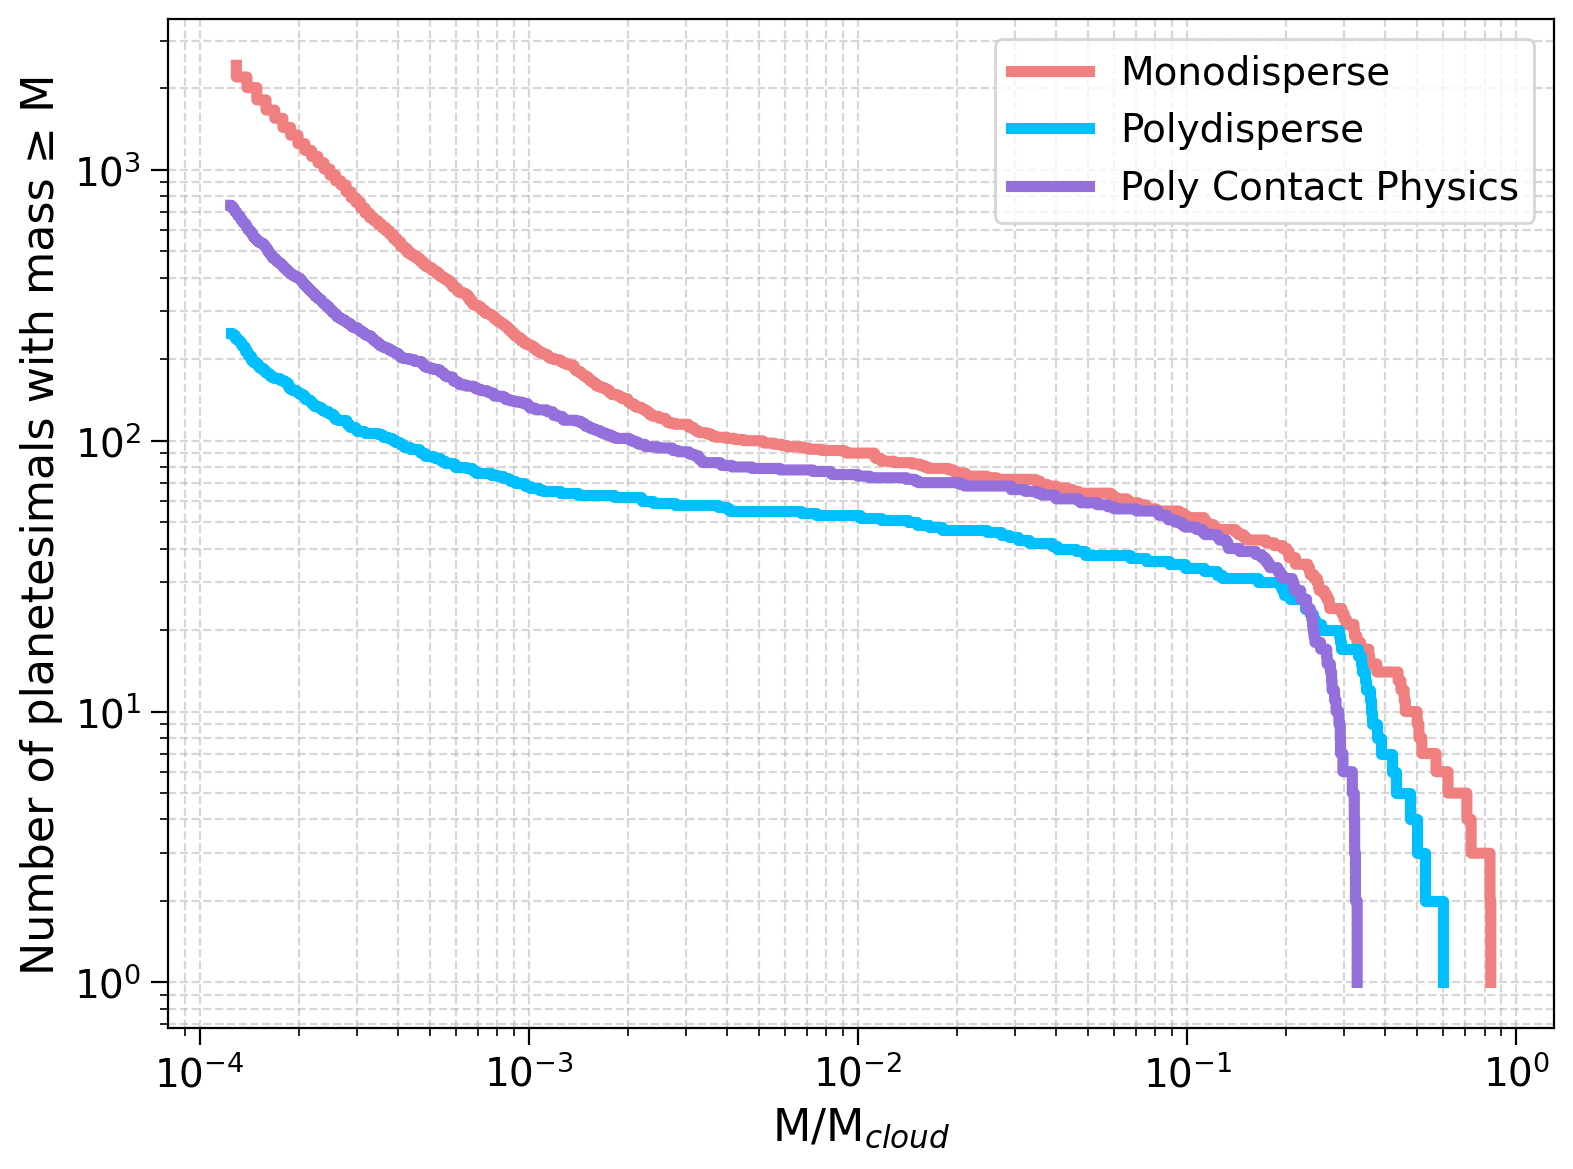
\includegraphics[width=\columnwidth]{figures/cumulative_mass_distribution_all.png}
    \caption{Cumulative number of planetesimals with mass $\geq M$ as
    a function of normalized mass $M/M_{\rm cloud}$, for the
    monodisperse (pink), polydisperse (blue), and polydisperse with
    contact-physics friction (purple) suites.}
    \label{fig:mass-function}
\end{figure}

Finally, Figure~\ref{fig:mass-function} places these binary and
primary-accretion results in the context of the overall planetesimal
population from which they are drawn. At the smallest resolved
masses, the monodisperse suite produces roughly an order of magnitude
more planetesimals than either polydisperse suite, consistent with
the larger number of binaries formed by monodisperse clouds in
Figure~\ref{fig:binary_formation_comparison}. The frictionless and
friction-included polydisperse suites track each other closely at low
mass but diverge at $M/M_{\rm cloud} \gtrsim 10^{-2}$, where the
friction-included suite falls below the frictionless one, indicating
that interparticle friction slightly suppresses the growth of the
largest bodies relative to the frictionless polydisperse case. All
three suites show a steep cutoff at high mass, with the monodisperse
suite extending to the largest normalized masses
($M/M_{\rm cloud} \sim 1$), consistent with the higher primary
accretion efficiencies reached by monodisperse collapses in
Figure~\ref{fig:rotation-vs-accretion}. Together, these results paint
a consistent picture: monodisperse clouds fragment into many more,
individually less efficient bodies and binaries, while polydisperse
clouds -- particularly when friction is included -- concentrate mass
more selectively, producing fewer but more distinctly bimodal
outcomes across binary efficiency, orbital inclination, and primary
accretion.


\begin{comment}
\subsubsection{Binary Formation Efficiency and Frequency}

\begin{figure*}
    \centering
    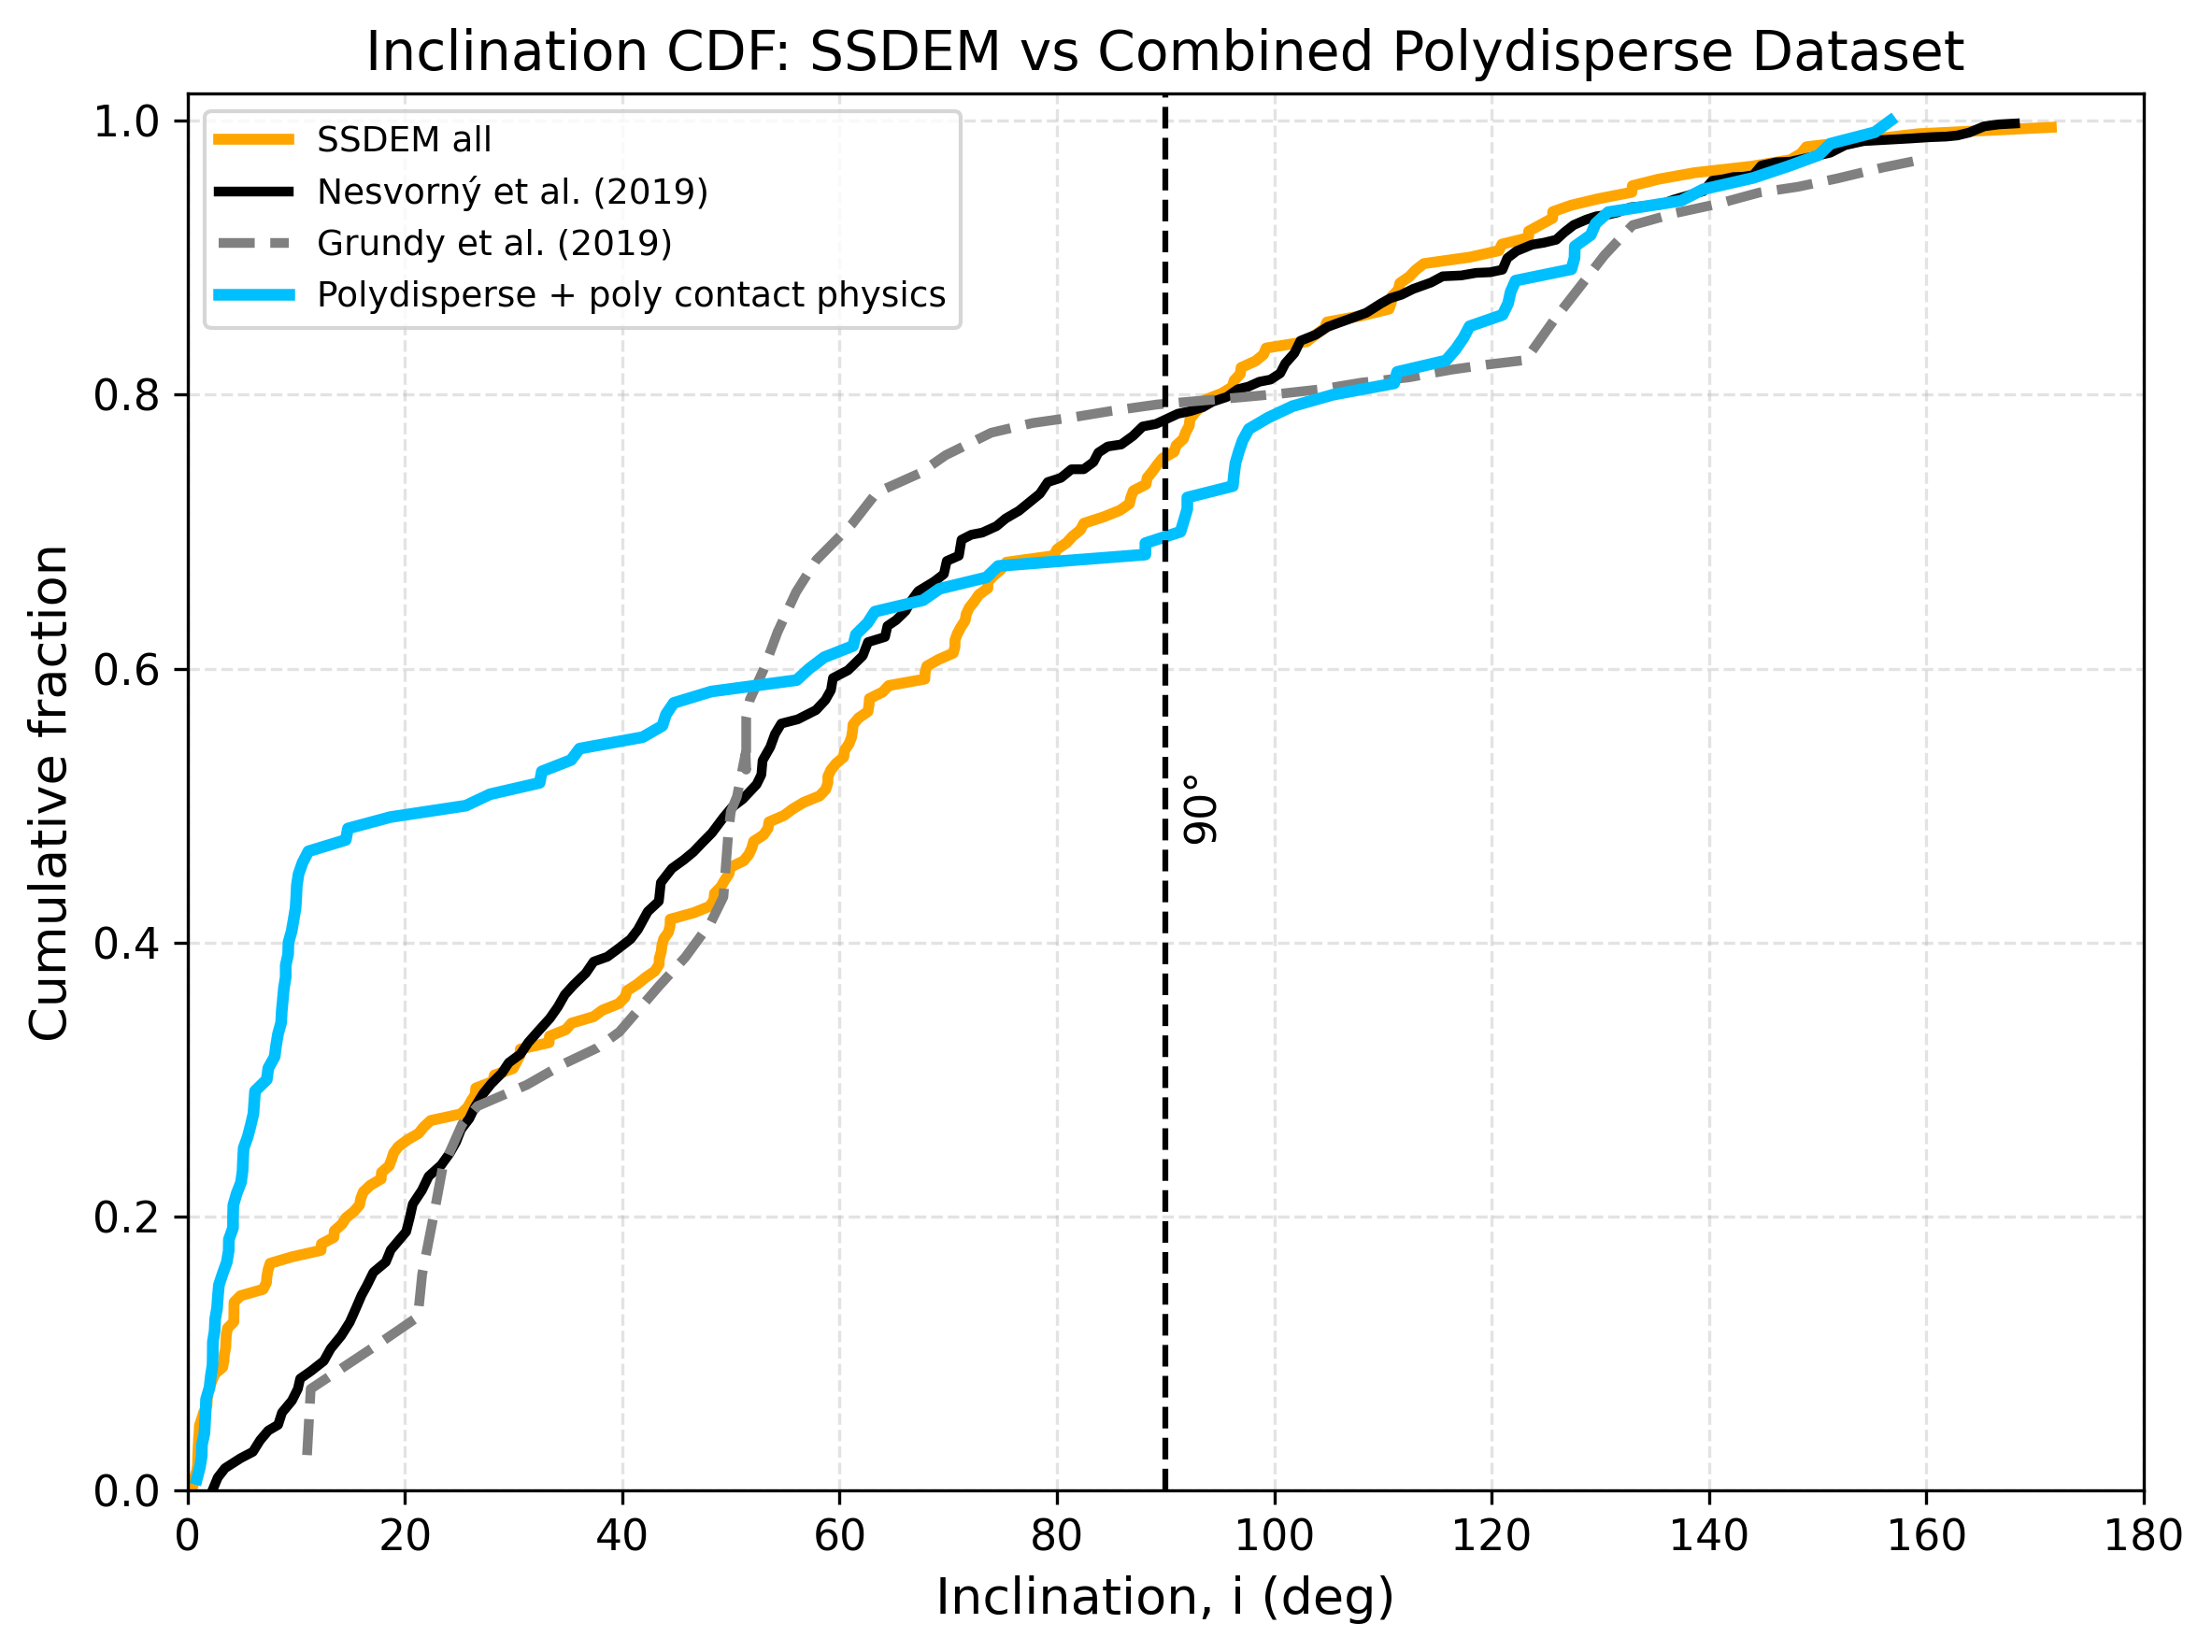
\includegraphics[width=\columnwidth]{figures/inc_cdf_ssdem_nesvorny_grundy_combined_poly.png}
    \caption{Cumulative fraction of binary planetesimals with
    inclination less than or equal to the value on the abscissa.
    Results from our polydisperse SSDEM simulations are shown in
    orange (full polydisperse binary dataset) and blue (polydisperse
    simulations including contact-physics friction), and are compared
    to the streaming-instability model of Nesvorn\'y et al. (2019,
    black) and the observed trans-Neptunian binaries of Grundy et al.
    (2019, gray dashed). The vertical dashed line at $90^\circ$
    indicates the separation between prograde and retrograde orbits.}
    \label{fig:inclination-cdf}
\end{figure*}

Figure~\ref{fig:inclination-cdf} compares the cumulative distribution
of inclinations for binary planetesimals formed in our polydisperse
SSDEM simulations to the streaming-instability model of
Nesvorn\'y et al. (2019) and the observed population of trans-Neptunian
binaries from Grundy et al. (2019). The orange curve, representing the
full polydisperse binary dataset, tracks the Nesvorn\'y et al. (2019)
distribution closely across most of the inclination range, and both
curves cross the $90^\circ$ line at a cumulative fraction of
$\approx 0.8$, indicating that roughly $80\%$ of binaries in both
datasets are prograde. The Grundy et al. (2019) observational sample
rises more steeply at low-to-intermediate inclinations
($i \lesssim 60^\circ$) before flattening out near $i \sim 90$--$130^\circ$,
reflecting a real population that is somewhat more concentrated toward
low-inclination, prograde orbits than either simulated dataset.

The polydisperse simulations including contact-physics friction (blue)
depart most noticeably from the other three curves at low inclination:
this population reaches a cumulative fraction of $\approx 0.5$ by
$i \sim 10^\circ$, far earlier than the orange SSDEM curve, the
Nesvorn\'y et al. (2019) model, or the observed Grundy et al. (2019)
sample, indicating that interparticle friction produces a substantially
larger fraction of low-inclination, nearly coplanar binaries than
either the frictionless polydisperse simulations or the observed
trans-Neptunian population. Beyond $i \sim 50^\circ$, however, the
friction-included curve flattens and largely converges with the
frictionless orange curve, crossing the $90^\circ$ line at a similar
cumulative fraction of $\approx 0.8$. This suggests that internal
friction primarily suppresses the formation of highly inclined
binaries at low inclination while leaving the overall
prograde/retrograde balance of the population largely unchanged.

\begin{figure*}
    \centering
    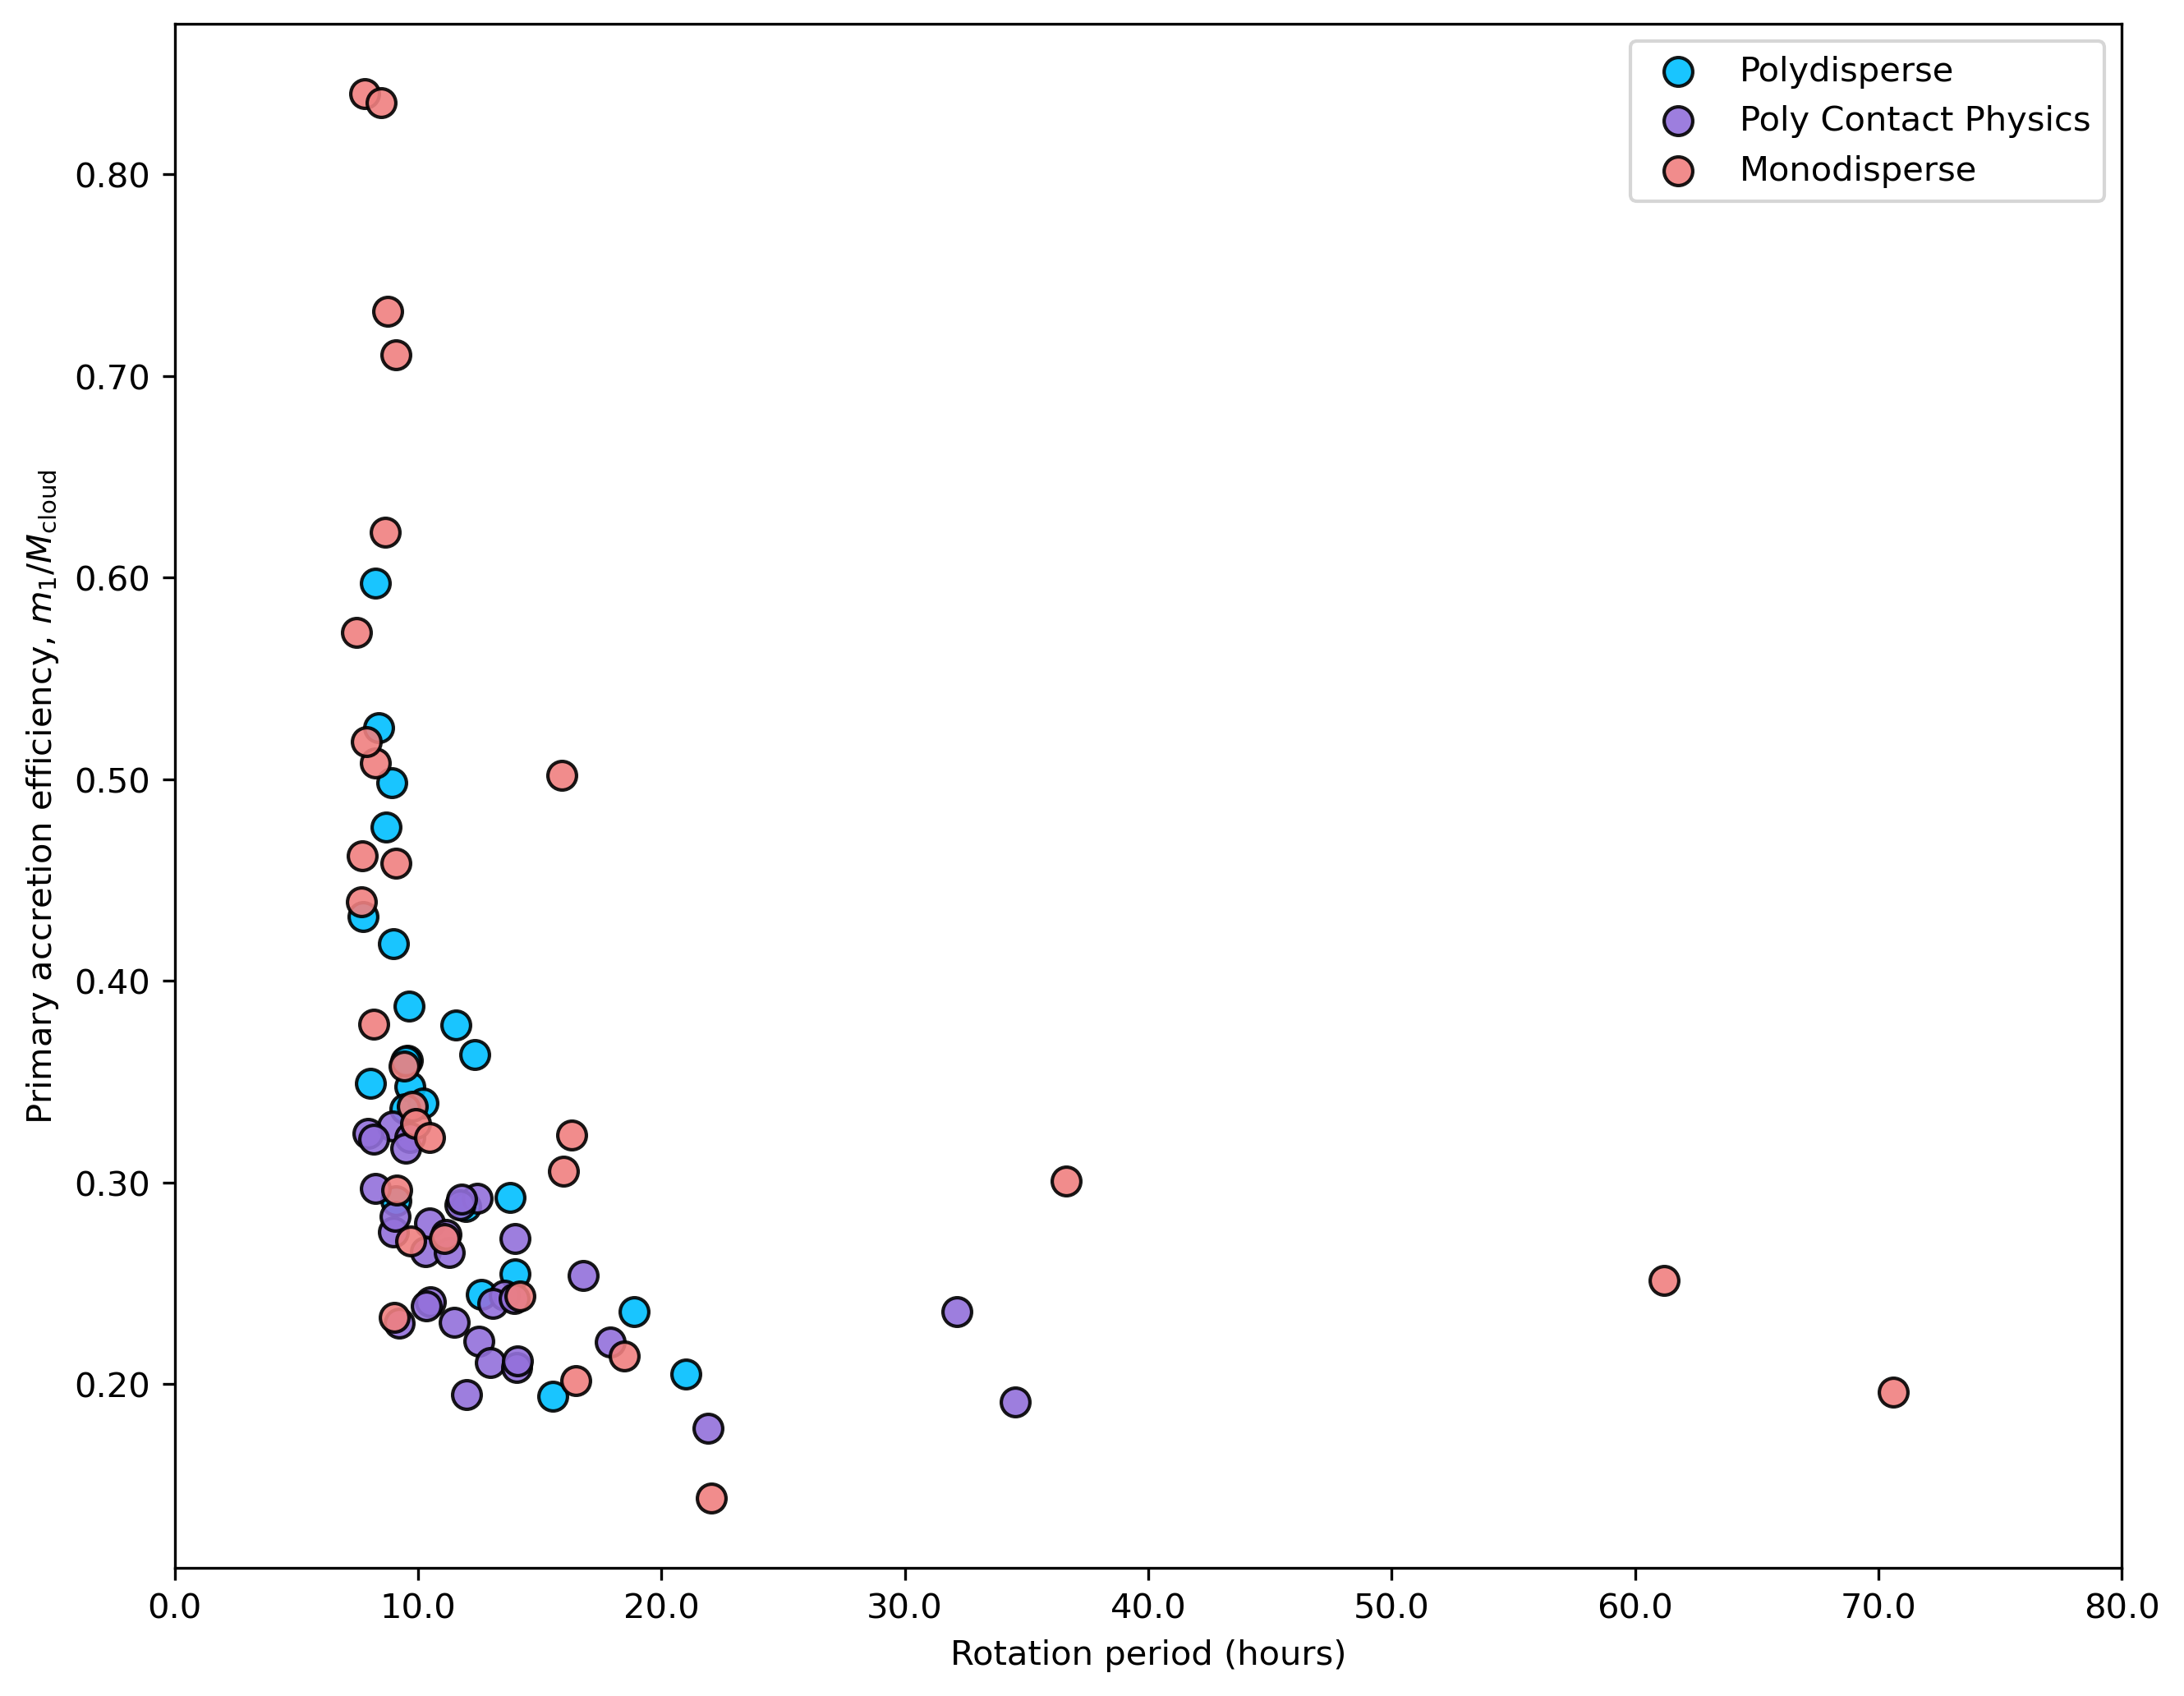
\includegraphics[width=\columnwidth]{figures/most_massive_rotation_vs_accretion.png}
    \caption{Primary accretion efficiency, $m_1/M_{\rm cloud}$, as a
    function of rotation period (hours) for the most massive
    planetesimal formed in each simulation. Blue points denote the
    polydisperse suite, purple points denote polydisperse simulations
    including contact-physics friction, and pink points denote the
    monodisperse suite.}
    \label{fig:rotation-vs-accretion}
\end{figure*}

Figure~\ref{fig:rotation-vs-accretion} shows the accretion efficiency
of the most massive planetesimal formed in each simulation,
$m_1/M_{\rm cloud}$, as a function of its rotation period. Across all
three suites, the highest accretion efficiencies ($m_1/M_{\rm cloud}
\gtrsim 0.5$) are achieved almost exclusively at short rotation
periods ($\lesssim 10$ hours), and efficiency falls off steeply as the
rotation period increases. The monodisperse population reaches the
highest efficiencies overall, with several simulations exceeding
$m_1/M_{\rm cloud} \approx 0.7$--$0.85$ at periods below $10$ hours.
The polydisperse population (without contact-physics friction) follows
a similar trend but does not reach quite as high an efficiency at
short periods, while still populating the same short-period,
high-efficiency region as the monodisperse suite. This indicates that,
for the most massive body formed in a given collapse, rapid final
rotation is closely associated with efficient mass capture, largely
independent of the particle-size distribution.

The polydisperse simulations that include contact-physics friction
depart most clearly from this pattern. These points are systematically
confined to a narrower range of rotation periods ($\sim 10$--$35$
hours) and to lower accretion efficiencies ($m_1/M_{\rm cloud}
\lesssim 0.3$), with no points reaching the high-efficiency,
short-period regime populated by the other two suites. This suggests
that interparticle friction suppresses the runaway accretion that
produces the most efficient primaries in the frictionless cases,
instead redistributing angular momentum and mass more evenly across
the collapsing cloud. At the longest rotation periods
($\gtrsim 40$ hours), only monodisperse simulations are present,
extending out to periods of $\sim 60$--$70$ hours at low efficiency
($m_1/M_{\rm cloud} \approx 0.2$--$0.3$); the absence of polydisperse
points in this regime may indicate that polydisperse collapses more
consistently avoid producing such slowly rotating, inefficient
primaries, though with the limited number of points here this should
be treated as suggestive rather than conclusive.

\begin{figure*}
    \centering
    % Polydisperse
    \begin{subfigure}{0.48\textwidth}
        \centering
        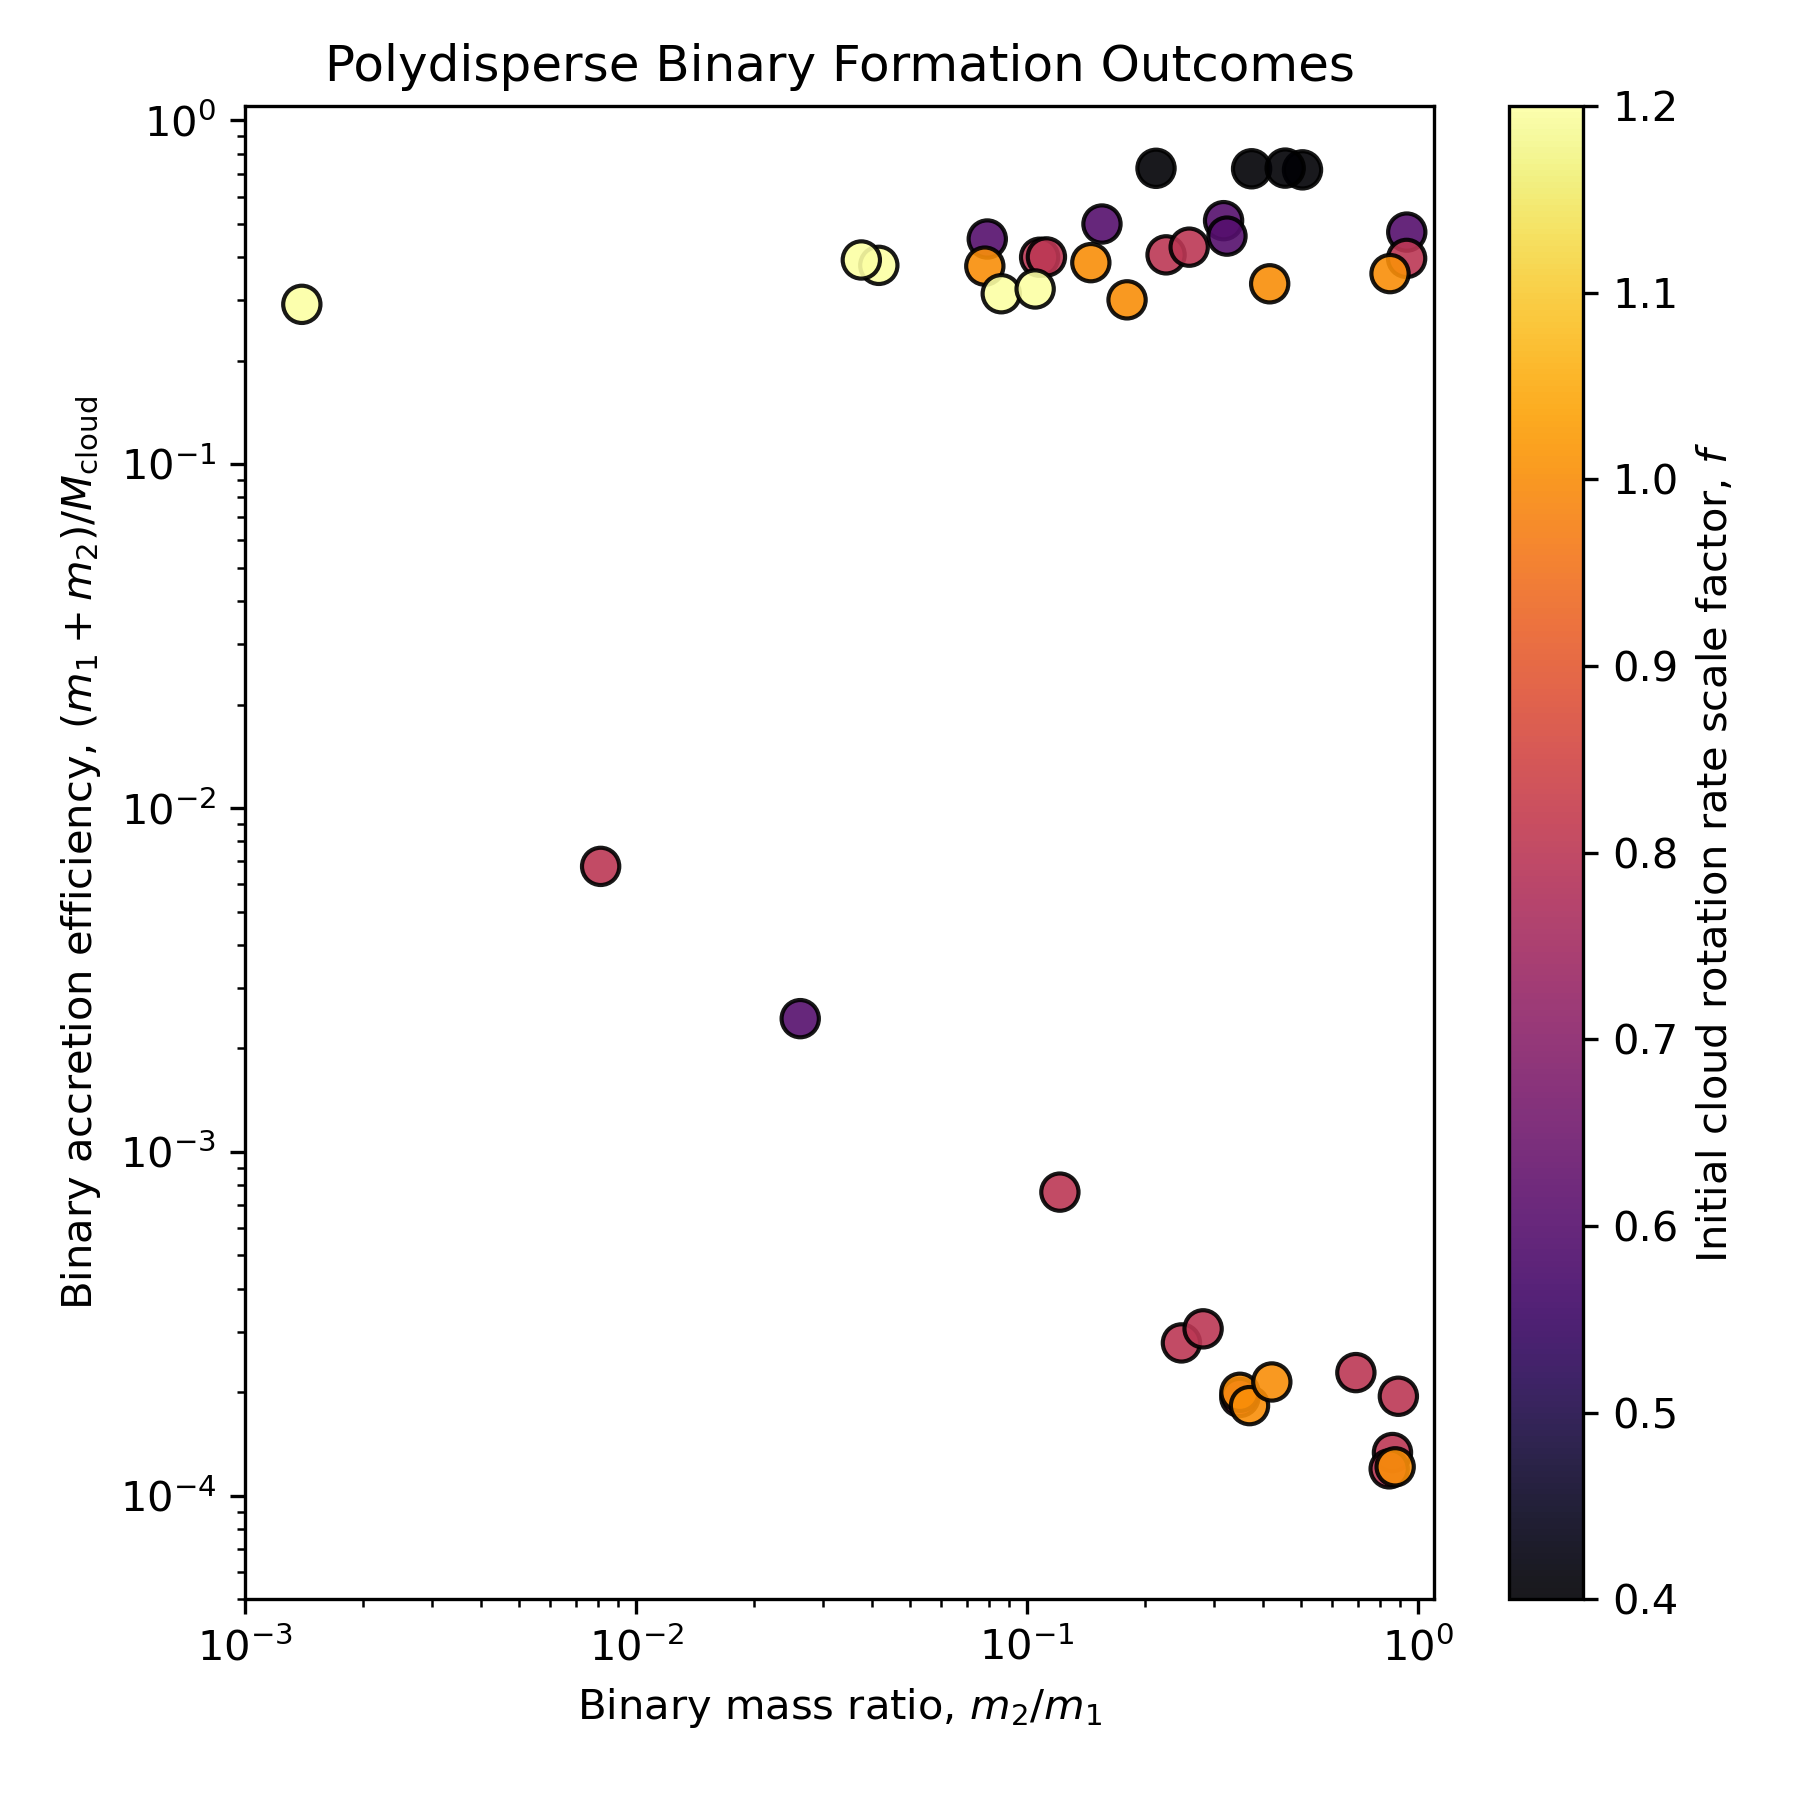
\includegraphics[width=\textwidth]{figures/binary_polydisperse.png}
        \caption{Polydisperse simulations: Binary accretion efficiency $(m_1 + m_2)/M_{\mathrm{cloud}}$ versus binary mass ratio $m_2/m_1$, with points colored by the initial cloud rotation rate scale factor $f$.}
        \label{fig:binary_polydisperse}
    \end{subfigure}
    \hfill
    % Monodisperse
    \begin{subfigure}{0.48\textwidth}
        \centering
        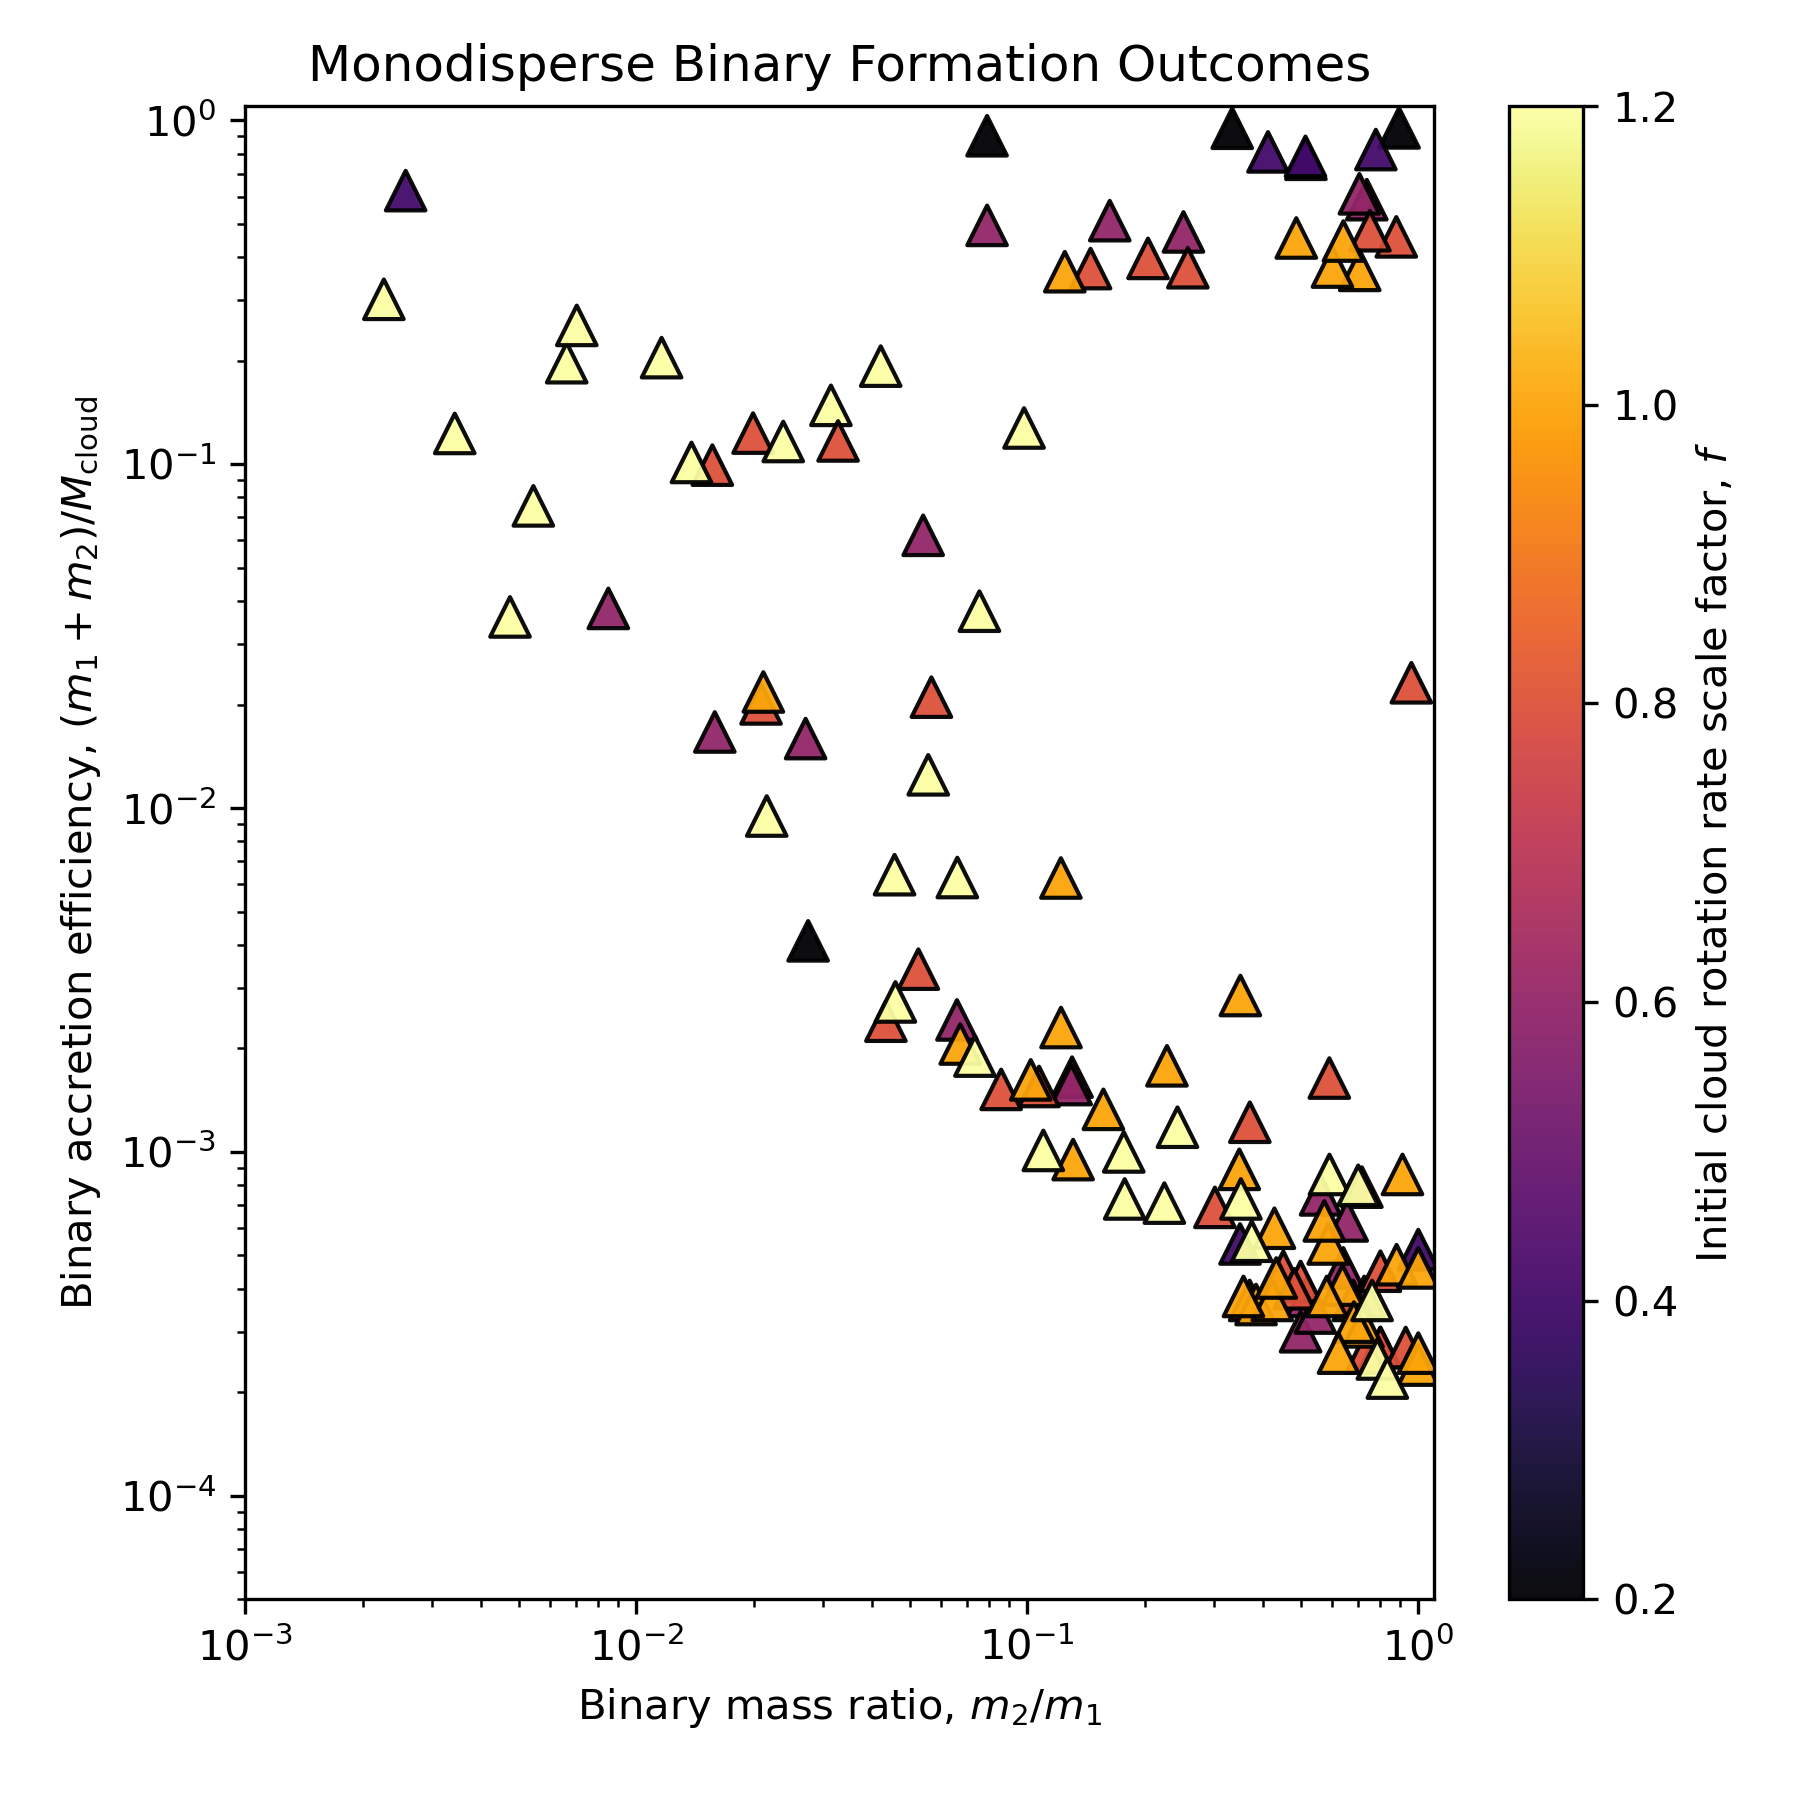
\includegraphics[width=\textwidth]{figures/binary_monodisperse.png}
        \caption{Monodisperse simulations: Same as Fig~\ref{fig:binary_polydisperse}, but for monodisperse particle distributions.}
        \label{fig:binary_monodisperse}
    \end{subfigure}
    %
    \caption{Comparison of binary formation outcomes in polydisperse (left) and monodisperse (right) gravitational collapse simulations. Each point represents a bound binary system, with marker color indicating the initial cloud rotation rate scale factor $ f$}
    \label{fig:binary_formation_comparison}
\end{figure*}


Each panel presents the outcome of multiple collapse simulations that resulted in bound binary systems. The horizontal axis shows the \textit{binary mass ratio}, $m_2/m_1$, where $m_1$ and $m_2$ represent the primary and secondary component masses, respectively. A value of $m_2/m_1 = 1$ corresponds to an equal-mass binary, while smaller values indicate systems in which the secondary component is significantly less massive than the primary. The vertical axis shows the \textit{binary accretion efficiency}, $(m_1 + m_2)/M_{\mathrm{cloud}}$, which quantifies the fraction of the total initial cloud mass that becomes bound in the binary system. Points are color-coded by the initial cloud rotation rate scale factor $f$, with darker colors corresponding to slower rotation and lighter colors representing more rapidly rotating initial conditions.

In the left panel, the results from \textbf{polydisperse simulations} are shown. These simulations begin with a range of particle sizes, which promotes a variety of local collapse behaviors and more efficient angular momentum redistribution. The binary accretion efficiencies remain relatively high, typically between $10^{-2}$ and $1$, across a broad range of mass ratios. This suggests that, even for systems with unequal component masses, a substantial fraction of the cloud mass can be captured into the binary. However, the number of points is comparatively smaller, indicating that while binaries in polydisperse simulations tend to be more massive and efficient, they are less frequent overall. The color trend suggests that rotation plays a secondary role here — faster rotating clouds (lighter colors) show slightly reduced efficiencies, but the overall range of outcomes remains narrow.

The right panel displays results from \textbf{monodisperse simulations}, where all particles begin with the same size and mass. In contrast to the polydisperse case, many more binary systems form, as evidenced by the larger number of data points. However, these binaries generally exhibit lower accretion efficiencies, particularly at small mass ratios.  A clear downward trend is observed: as $m_2/m_1$ decreases, $(m_1 + m_2)/M_{\mathrm{cloud}}$ drops by several orders of magnitude, reaching values as low as $10^{-4}$.  This indicates that monodisperse clouds form numerous, but less massive, binary systems.  The color gradient reveals that faster-rotating clouds (lighter colors) tend to form binaries with especially low efficiencies, suggesting that rotation inhibits the collapse and accretion processes when the particle population is uniform.

Taken together, these results show that particle size diversity strongly influences both the \textit{frequency} and \textit{efficiency} of binary formation. Polydisperse clouds form fewer, but more massive and efficient, binaries, likely due to enhanced angular-momentum transport enabled by size variation.  Monodisperse clouds, on the other hand, produce a larger number of binaries, but each tends to capture a smaller fraction of the available mass, reflecting less effective accretion under uniform conditions. These findings highlight the importance of particle size distribution in shaping the multiplicity and mass distribution of binaries produced during gravitational collapse.
\end{comment}

\begin{table}
\centering
\caption{Average number of binaries  with $m_1 \geq 1\times10^{-16}$ and $m_2 \geq$ $8\times10^{-17}$ , single planetesimals, and planetesimals $\geq$ $8\times10^{-17}$ for each Eccentricity and U combination.}
\label{tab:planetesimals_averages}
\begin{tabular}{c c c c c }
\toprule
$\varepsilon$ & $\mu$ & {Avg. Binaries} & {Avg. Singles} & {Avg. Planetesimals} \\
\midrule
\multirow{4}{*}{0.5}  & 0   & 3.6   & 125    & 131.2  \\
                      & 0.5 & 3.8   & 223.2  & 228.2  \\
                      & 1.0 &  2.75 & 225.75 & 231.25 \\
                      & 2.0 &  2.2  & 230.2  & 234.2  \\
\midrule
\multirow{3}{*}{0.7}  & 0   & 2.2 & 94     & 98    \\
                      & 0.5 & 3.2 & 200.4  & 205.8 \\
                      & 1.0 & 3   & 199.75 & 205.5 \\
\bottomrule
\end{tabular}
\end{table}

\begin{table}
\centering
\caption{Average number of binaries with $m_1 \geq 1\times10^{-16}$ and $m_2 \geq$ $8\times10^{-17}$, single planetesimals, and planetesimals $ \geq 8\times10^{-17}$ for each suite.}
\label{tab:suites_averages}
\begin{tabular}{c c c c}
\toprule
Suite & {Avg. Binaries} & {Avg. Singles} & {Avg. Planetesimals} \\
\midrule
0.4x & 1.0 & 6.75  & 8.75  \\
0.6x & 1.4 & 21.8  & 24.4  \\
0.8x & 3.6 & 87.00 & 93.4  \\
1.0x & 2.0 & 104.8 & 108.6 \\
1.2x & 1.4 & 67.8  & 70.2  \\
\bottomrule
\end{tabular}
\end{table}

The binary statistics make it clear that particle-size diversity changes not only the efficiency of mass capture but also the number and type of binaries formed. To understand whether this difference also extends to the morphology of individual planetesimals, we now turn to their overall shape classification.
\subsubsection{Shape Classification and Diversity}
\begin{figure}
    \centering
    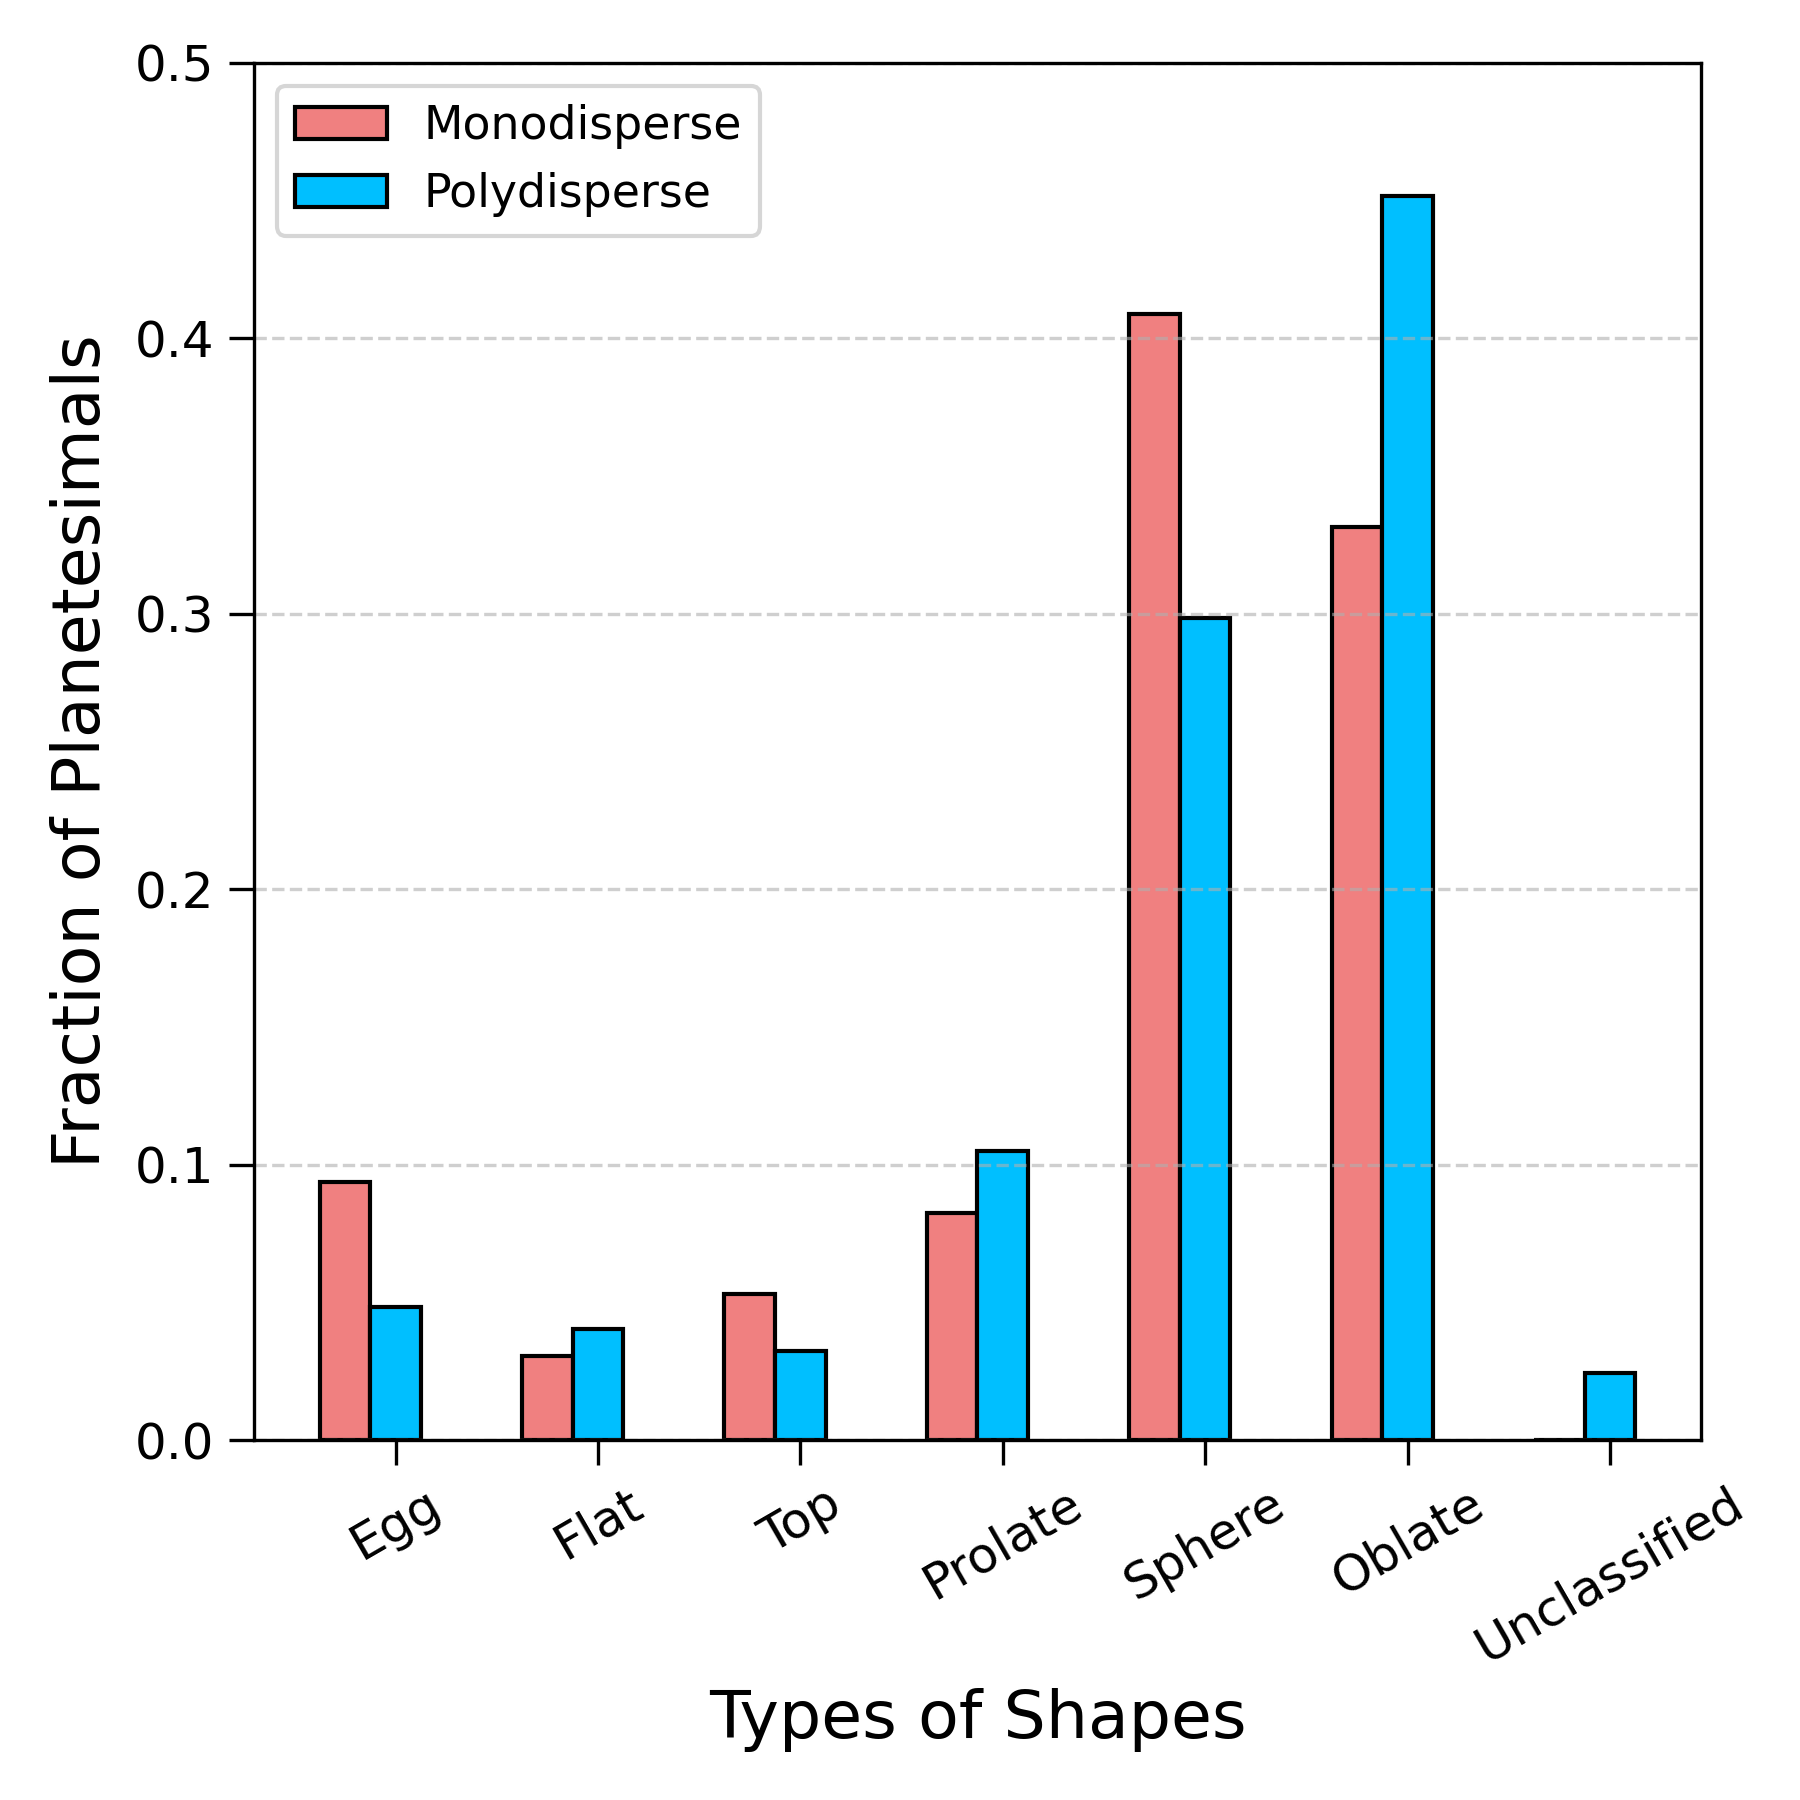
\includegraphics[width=\columnwidth]{figures/shape_distribution_comparison (2).png}
    \caption{Normalized shape distribution of planetesimals in monodisperse (red) and polydisperse (blue) simulations. The six shape categories are: Spherical, Top-shaped, Oblate, Egg-shaped, Flattened, and Unclassified.}
    \label{fig:shapes_classification}
\end{figure}

Figure~\ref{fig:shapes_classification} presents the normalized
distribution of planetesimal shapes derived from the monodisperse and
polydisperse simulations. The x-axis categorizes planetesimals into
seven shape classes -- Egg, Flat, Top, Prolate, Sphere, Oblate, and
Unclassified -- based on their geometric ratios, while the y-axis
shows the fraction of planetesimals belonging to each class. The pink
and blue bars correspond to monodisperse and polydisperse simulations,
respectively. This comparison illustrates how differences in the
initial particle size distribution affect the overall morphological
outcomes of gravitational collapse.

In both simulations, spherical and oblate shapes dominate the
population, indicating that most planetesimals form as nearly round
or mildly flattened objects. However, the relative fractions differ:
the monodisperse population yields a higher fraction of nearly
spherical planetesimals ($\approx 0.41$) than the polydisperse
population ($\approx 0.30$), whereas the polydisperse population
produces a higher fraction of oblate bodies ($\approx 0.45$) compared
to the monodisperse case ($\approx 0.33$). This difference suggests
that when particles of varying sizes collapse together, local
variations in mass density and angular momentum lead to asymmetric
compaction, favoring the formation of more flattened structures
relative to the monodisperse case.

The remaining shape categories -- Egg, Flat, Top, and Prolate -- each
account for a modest fraction of the population ($\lesssim 0.1$) in
both suites, representing more dynamically evolved outcomes that
typically arise from stronger rotational effects or uneven mass
distribution during collapse. The monodisperse population shows a
somewhat higher fraction of egg-shaped and top-shaped bodies, while the
polydisperse population shows a slightly higher fraction of prolate
and flattened bodies, though these differences are small compared to
the dominant sphere/oblate categories. The "unclassified" category
appears only in the polydisperse population, accounting for a small
but non-negligible fraction ($\approx 0.02$) of bodies that deviate
significantly from the simple axisymmetric shape classes, reflecting
the greater morphological irregularity introduced by particle-size
diversity.

Overall, the figure shows that particle size diversity shifts the
balance of planetesimal morphology away from purely spherical bodies
and toward oblate and irregular shapes. Monodisperse systems evolve
toward smoother, more symmetric bodies, while polydisperse systems
produce a somewhat broader and more irregular range of shapes. This
behavior underscores the role of size-dependent gravitational
clustering and angular momentum exchange during collapse, processes
that may explain the variety of shapes observed among asteroids and
other small Solar System bodies.

The broader range of shapes seen in polydisperse simulations supports
the idea that size diversity promotes irregular collapse and
asymmetry. To quantify these trends more precisely, we examine the
direct correlation between the two principal shape parameters --
oblateness and prolateness.

\subsubsection{Prolateness vs Oblateness}

\begin{figure}
    \centering
    \includegraphics[width=\columnwidth]{figures/prolateness_vs_oblateness.png}
    \caption{Prolateness ($\beta$ = 1 -- b/a) versus oblateness ($\gamma$ = 1 -- c/a) for planetesimals formed in both polydisperse and monodisperse simulations across different initial rotation rate scale factors ($f$). Each subplot represents a distinct $f$ value for the polydisperse case, while the bottom-right panel shows the combined monodisperse population. The symbols represent individual planetesimals, and color variations correspond to different spin rates. The figure highlights how increasing the initial spin factor affects the overall shape distribution, with trends toward more elongated or flattened bodies depending on initial cloud rotation and particle-size diversity.}
    \label{fig:prolateness_vsoblateness}
\end{figure}

Figure~\ref{fig:prolateness_vsoblateness} compares the prolateness ($\beta$ = 1 -- b/a) and oblateness ($\gamma$ = 1 -- c/a) of planetesimals formed in simulations with different initial rotation rate scale factors ($f$). The horizontal axis measures oblateness, representing how flattened a body is along its rotation axis, while the vertical axis measures prolateness, indicating how elongated it is along the major axis. Together, these shape parameters describe whether a planetesimal is more disk-like, cigar-like, or nearly spherical. Each point on the scatter plots corresponds to a single planetesimal identified in the simulation.

The top and bottom-left panels correspond to the polydisperse simulations at different spin factors ($f = 0.4x$, $0.6x$, $0.8x$, $1.0x$, and $1.2x$), while the bottom-right panel shows the monodisperse case. In the low-spin scenarios ($f = 0.4x$ and $0.6x$), most planetesimals cluster near the origin, with small $\beta$ and $\gamma$ values, indicating nearly spherical shapes. This reflects the slow rotation of the initial cloud, which allows self-gravity to dominate over rotational deformation. As $f$ increases, the distributions shift toward larger oblateness and prolateness, implying that faster initial rotation promotes more aspherical and flattened bodies.

At higher spin factors ($f \geq 0.8x$), the polydisperse populations display a broader scatter, with some planetesimals reaching high prolateness and oblateness simultaneously. This behavior suggests that strong rotation and a diverse size distribution enhance non-axisymmetric collapse, producing triaxial or irregularly elongated shapes. In contrast, the monodisperse case exhibits a tight linear correlation between $\beta$ and $\gamma$, indicating that shape deformation proceeds in a more uniform and axisymmetric way when all particles have similar sizes. The lack of scatter in this case highlights the stabilizing effect of uniform particle size on the collapse geometry.

Overall, the figure demonstrates that both the initial spin factor and particle-size diversity play critical roles in shaping the final morphology of planetesimals. Higher spin leads to more elongated and flattened structures, while polydispersity introduces shape variability by enabling more complex collapse dynamics. These results suggest that observed diversity in asteroid shapes could naturally arise from variations in the initial spin and particle size distributions of the collapsing parent clouds.

These shape correlations confirm that monodisperse systems deform more uniformly, while polydisperse ones show greater irregularity and scatter, consistent with more complex collapse dynamics. Because many of these shapes occur in binaries, it is natural to next examine how such internal and morphological differences influence binary orbital properties.

\begin{figure}
    \centering
    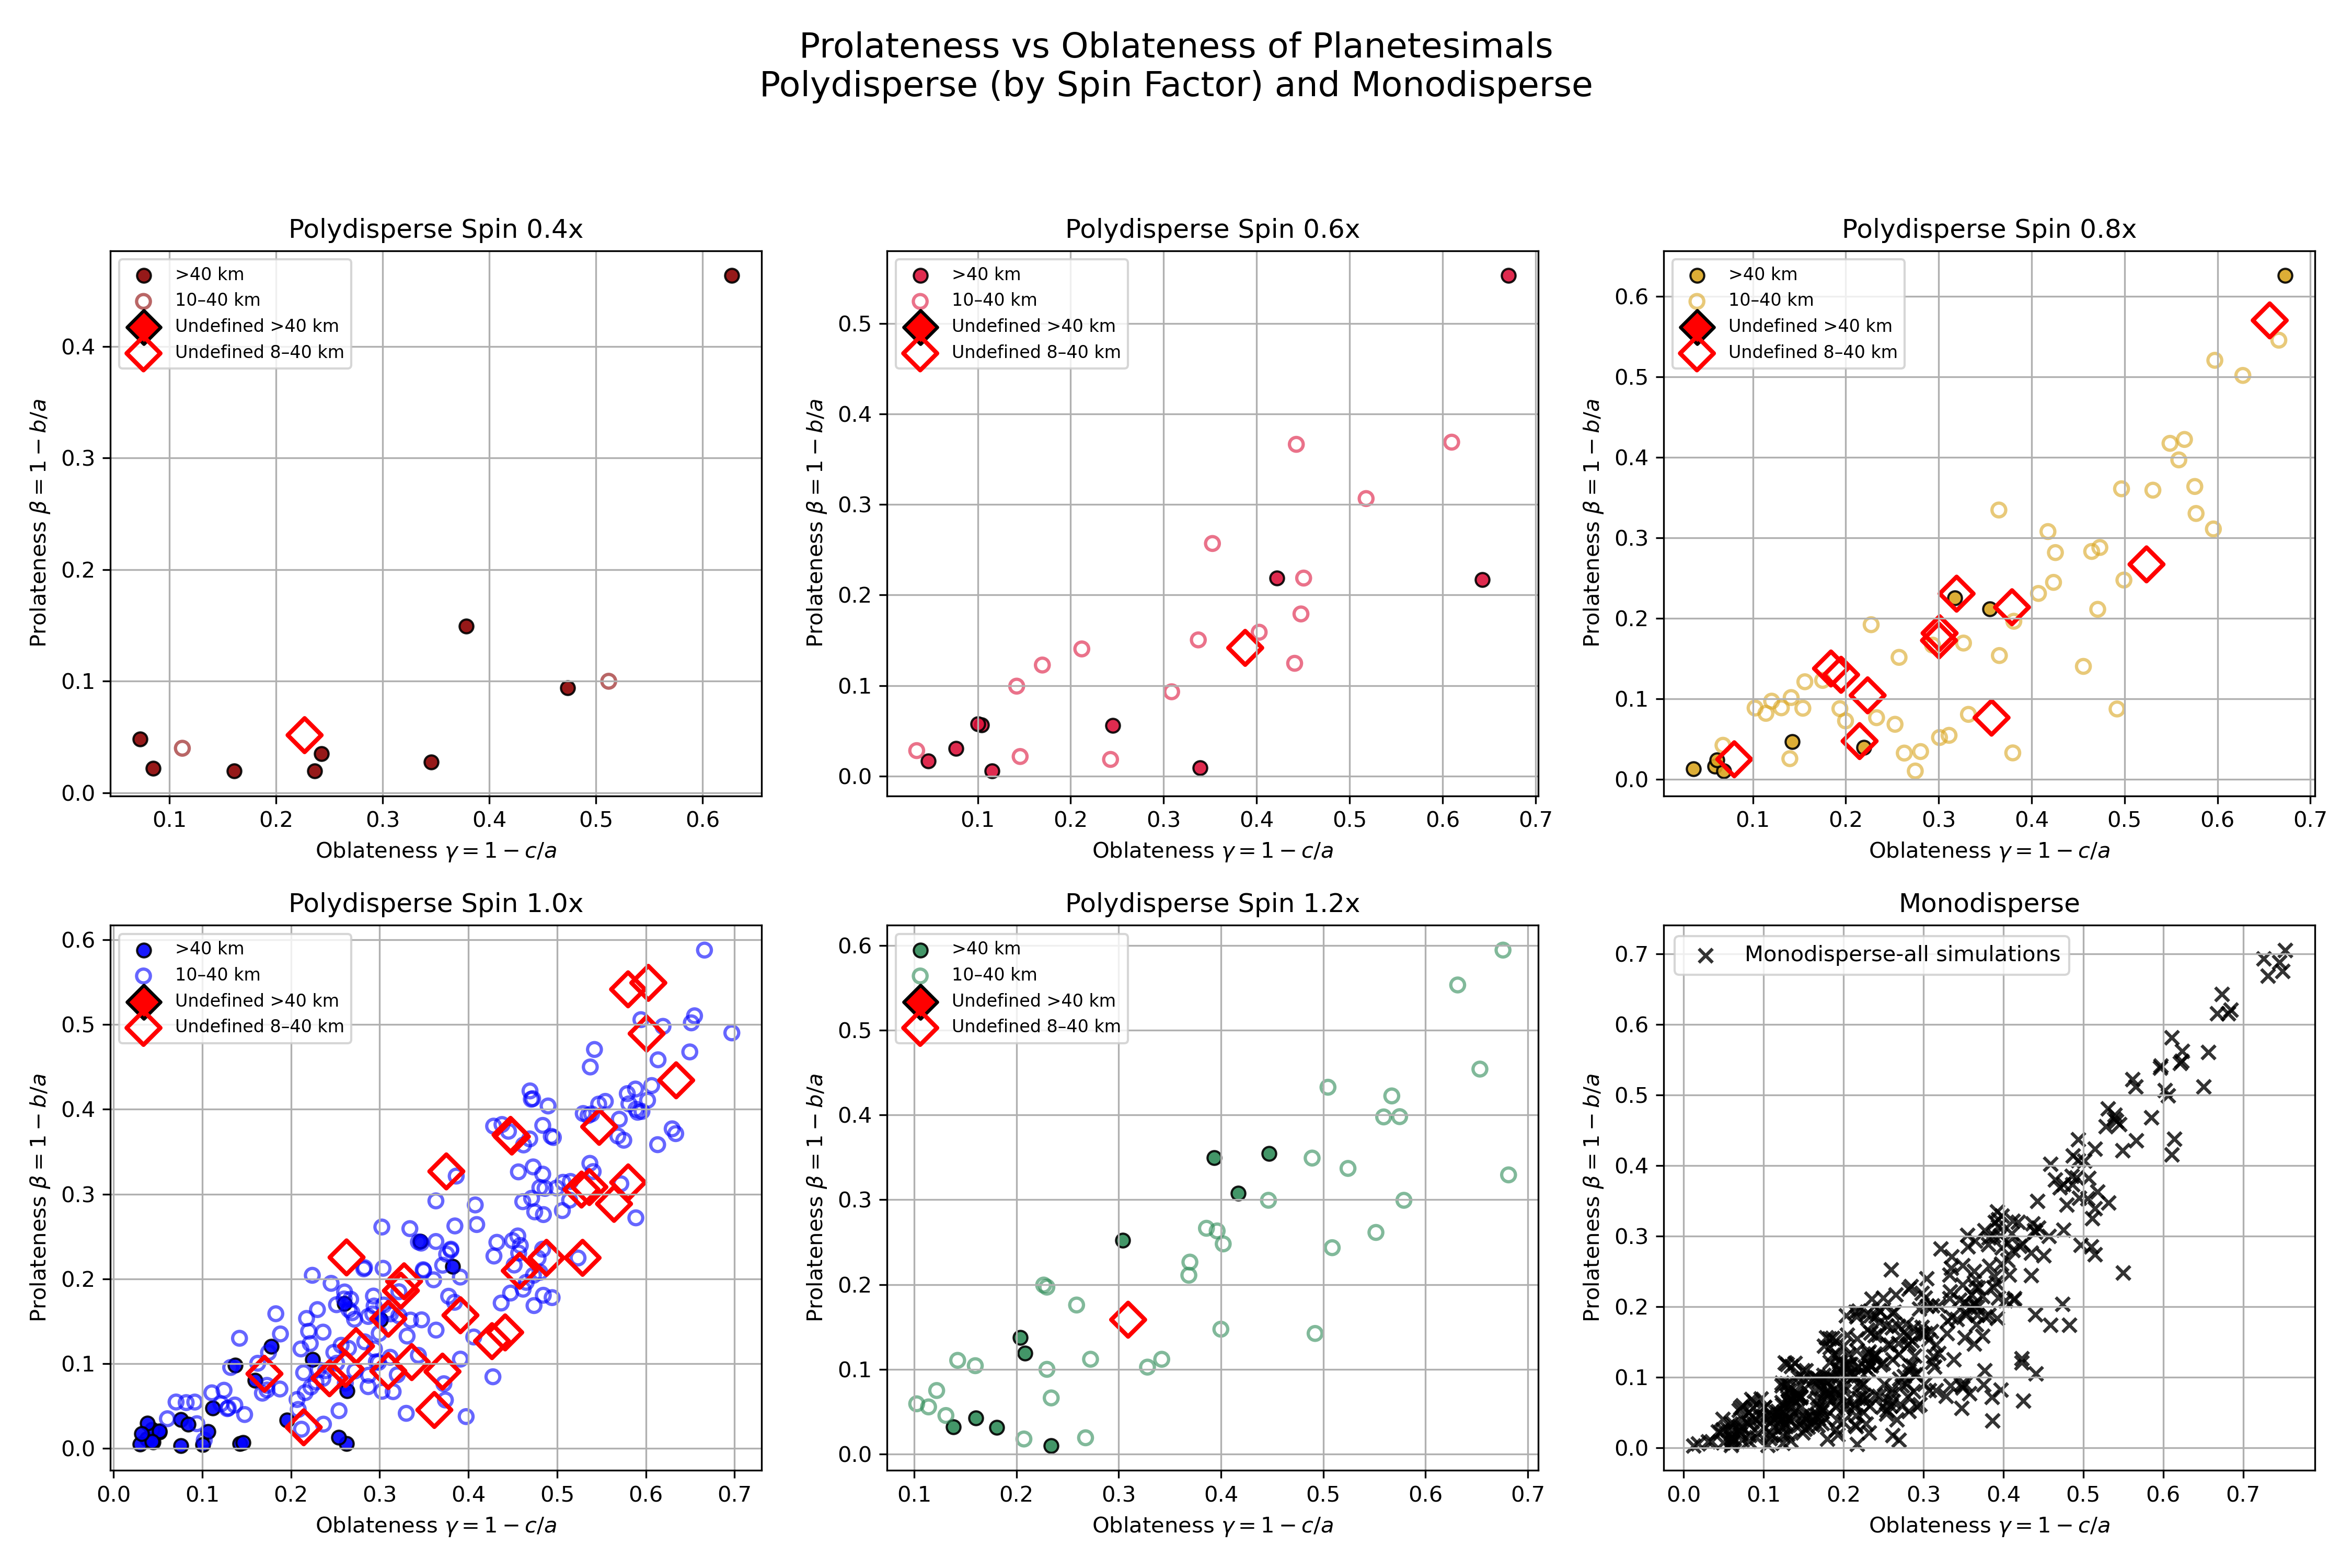
\includegraphics[width=\columnwidth]{figures/prolateness_vs_oblateness_undefined.png}
    \caption{}
    \label{fig:prolateness_vsoblateness_undefined}
\end{figure}

\begin{figure}
    \centering
    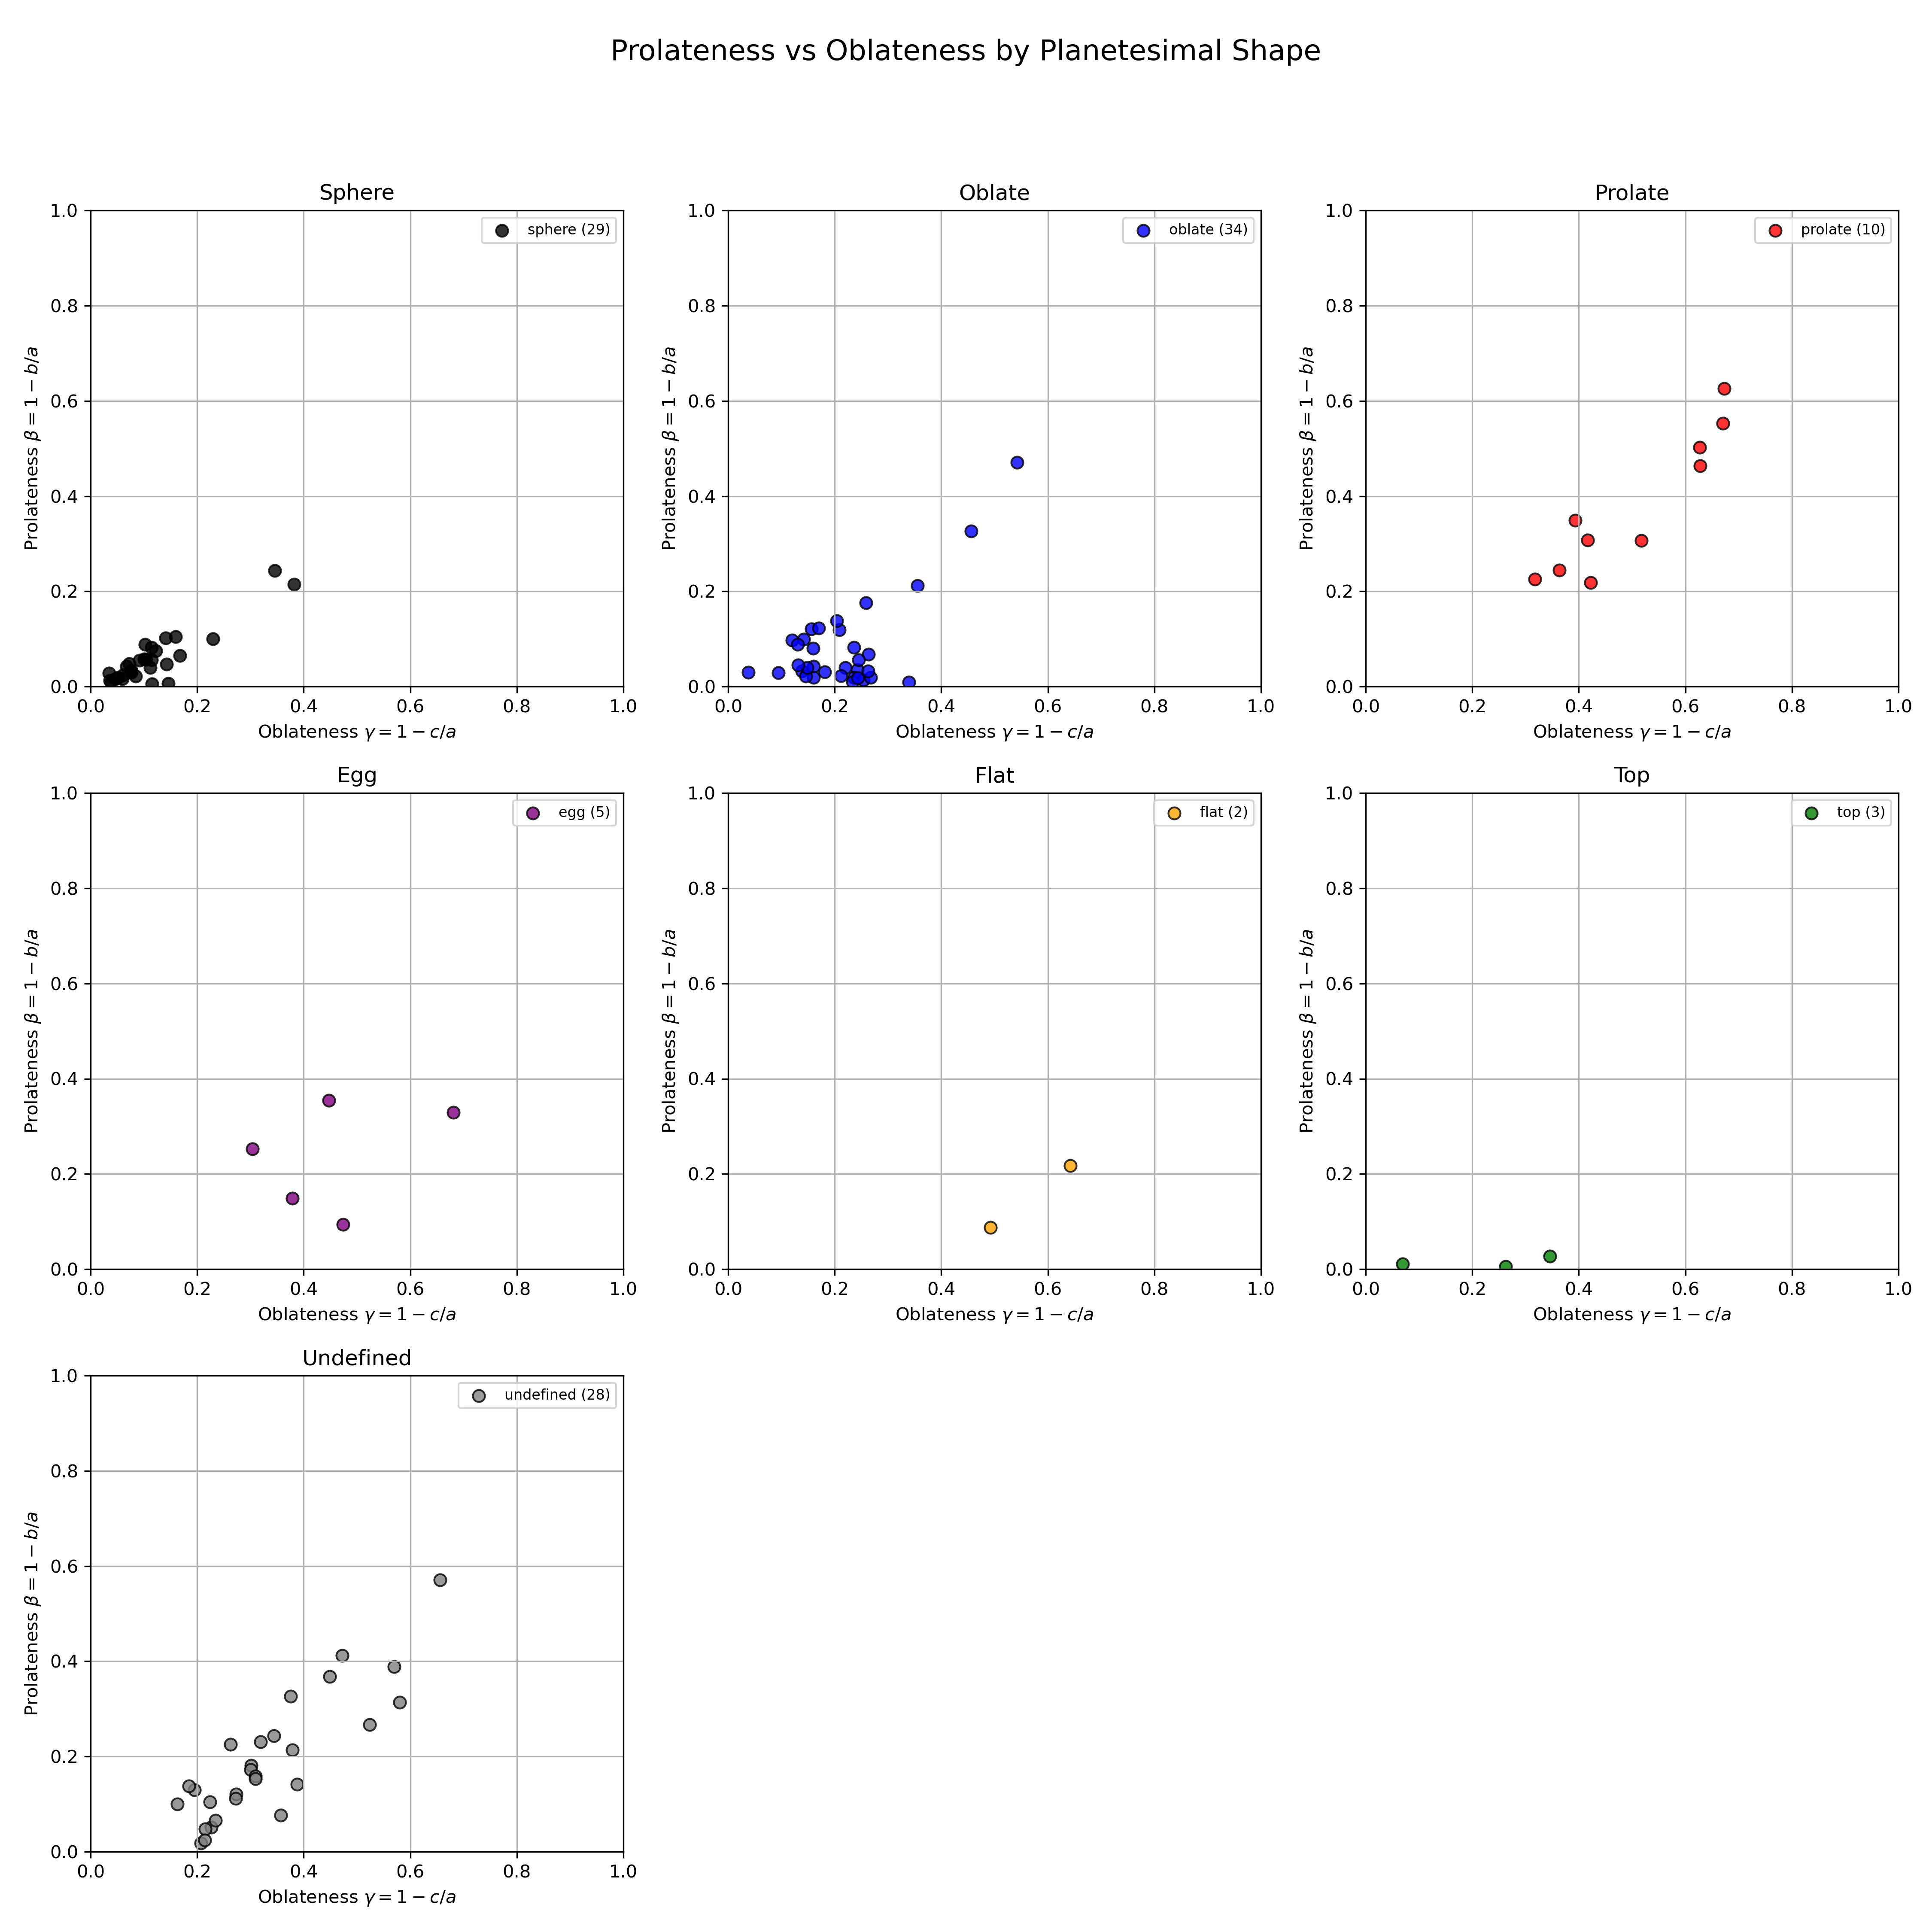
\includegraphics[width=\columnwidth]{figures/prolateness_vs_oblateness_by_shape.png}
    \caption{}
    \label{fig:prolateness_vsoblateness_undefined}
\end{figure}

\subsubsection{Binary Orbital Properties}
\begin{figure*}
    \centering
    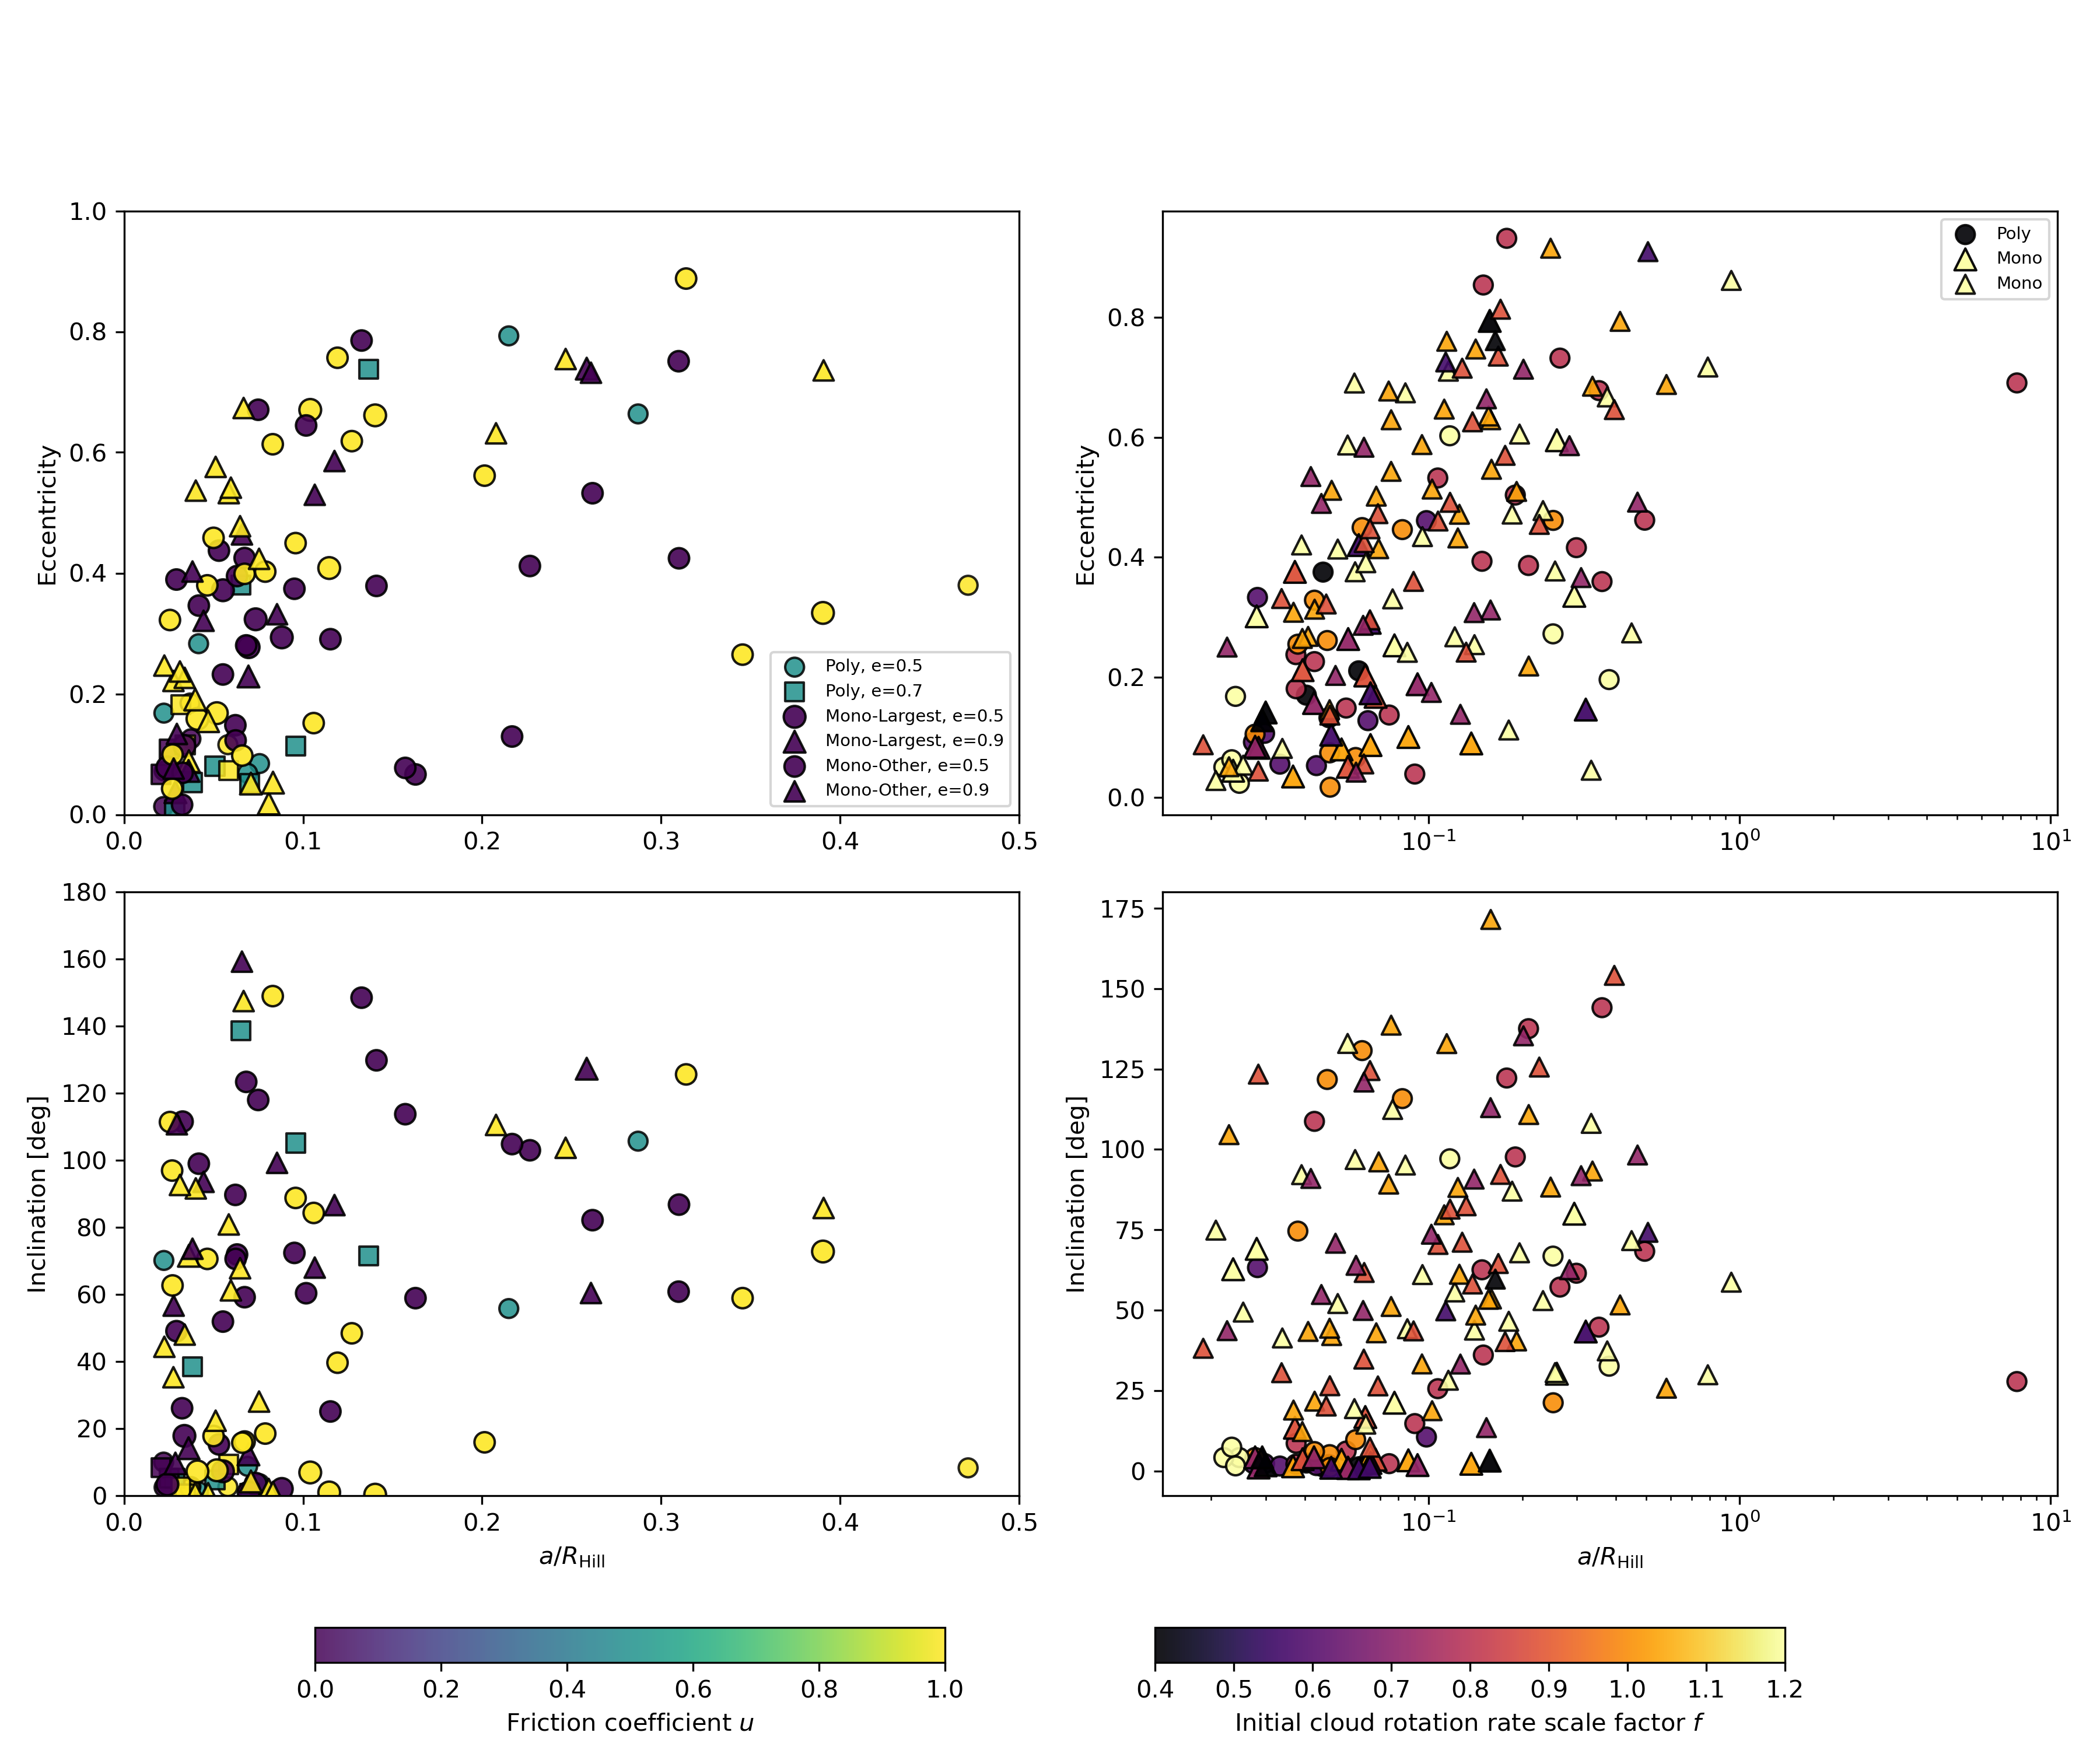
\includegraphics[width=\textwidth]{figures/Inc_Ecc_vs_a_Rhill.png}
    \caption{Orbital properties of planetesimal binaries from monodisperse (triangles) and polydisperse (circles/squares) simulations. Top row: eccentricity versus mutual semi-major axis normalized by the Hill radius ($a/R_{\mathrm{Hill}}$). Bottom row: inclination versus $a/R_{\mathrm{Hill}}$. Left column: symbols colored by friction coefficient $u$; right column: symbols colored by initial cloud rotation rate scale factor $f$. Different marker styles denote monodisperse and polydisperse cases as indicated in the legend.}
    \label{fig:inc_ecc_a_Rhill}
\end{figure*}
Figure~\ref{fig:inc_ecc_a_Rhill} compares the orbital characteristics of planetesimal binaries formed in monodisperse and polydisperse collapse simulations. The top row shows the binary eccentricity as a function of the mutual semi-major axis normalized by the Hill radius, $a/R_{\mathrm{Hill}}$, while the bottom row presents the inclination relative to the initial cloud rotation axis. The left column displays results color-coded by the friction coefficient $u$, which measures the degree of collisional dissipation during the collapse, and the right column shows results color-coded by the initial cloud rotation rate scale factor $f$. Triangles correspond to binaries from monodisperse simulations, and circles or squares denote those from polydisperse runs.

The panels colored by the friction coefficient $u$ (left column) reveal a clear correlation between dissipative strength and orbital compactness. Systems with higher $u$ values (lighter colors) tend to occupy the lower portion of the plot, corresponding to smaller $a/R_{\mathrm{Hill}}$ and lower eccentricities. This indicates that stronger frictional coupling promotes energy loss during encounters, allowing planetesimals to settle into more tightly bound and circular orbits. In contrast, binaries formed in low-friction environments (darker points) are typically found at larger separations and exhibit higher eccentricities, implying that limited dissipation leaves them in dynamically excited states. This trend is consistent for both monodisperse and polydisperse cases, though the latter show a stronger concentration of high-$u$ systems at small separations, suggesting that polydispersity enhances effective damping through more frequent or uneven particle interactions.

The panels on the right, colored by the initial rotation rate factor $f$, show how global angular momentum affects these same orbital properties. Here, faster-rotating clouds (lighter colors) tend to produce binaries with larger $a/R_{\mathrm{Hill}}$ and higher eccentricities. This pattern indicates that rotational support counteracts collapse and reduces the ability of the cloud to form compact binaries, leading to systems that are more weakly bound and dynamically excited. The effect is especially pronounced in monodisperse simulations, where limited internal dissipation means that much of the initial rotational energy is retained in orbital motion rather than being radiated away through collisions.

When comparing the two particle distributions, a consistent contrast emerges. Monodisperse simulations form a larger number of binaries (as seen from the dense clustering of triangular symbols), but these tend to be wider, more eccentric, and more inclined. Many occupy the range $a/R_{\mathrm{Hill}} \gtrsim 10^{-1}$ with eccentricities $e \gtrsim 0.4$, reflecting dynamically hotter systems that form under less dissipative conditions. Polydisperse simulations, on the other hand, produce fewer binaries overall but with lower $a/R_{\mathrm{Hill}}$, smaller eccentricities, and inclinations mostly below $40^\circ$. This indicates that a range of particle sizes enhances angular momentum transfer and collisional damping, promoting the formation of compact, nearly coplanar binaries.

Overall, Figure~\ref{fig:inc_ecc_a_Rhill} shows that both the degree of frictional dissipation and the initial rotational state of the cloud play critical roles in determining the final orbital configuration of planetesimal binaries. High friction coefficients and moderate rotation favor the formation of tight, low-eccentricity binaries, particularly in polydisperse environments, while low friction and rapid rotation lead to a larger number of wide, eccentric, and inclined binaries, characteristic of the monodisperse simulations. These results emphasize that the interplay between microphysical dissipation and global rotation governs not only whether binaries form, but also the dynamical architectures they inherit from their parent clouds.
In summary, the comparison between monodisperse and polydisperse systems shows consistent rotational behavior but markedly different densities, morphologies, and binary characteristics. Finally, we isolate one additional factor—internal friction—to understand how material properties further modify these trends within the polydisperse systems.

\subsection{Internal Friction Effects in Polydisperse Systems}\label{sec:friction_effects}
\begin{figure*}
    \centering
    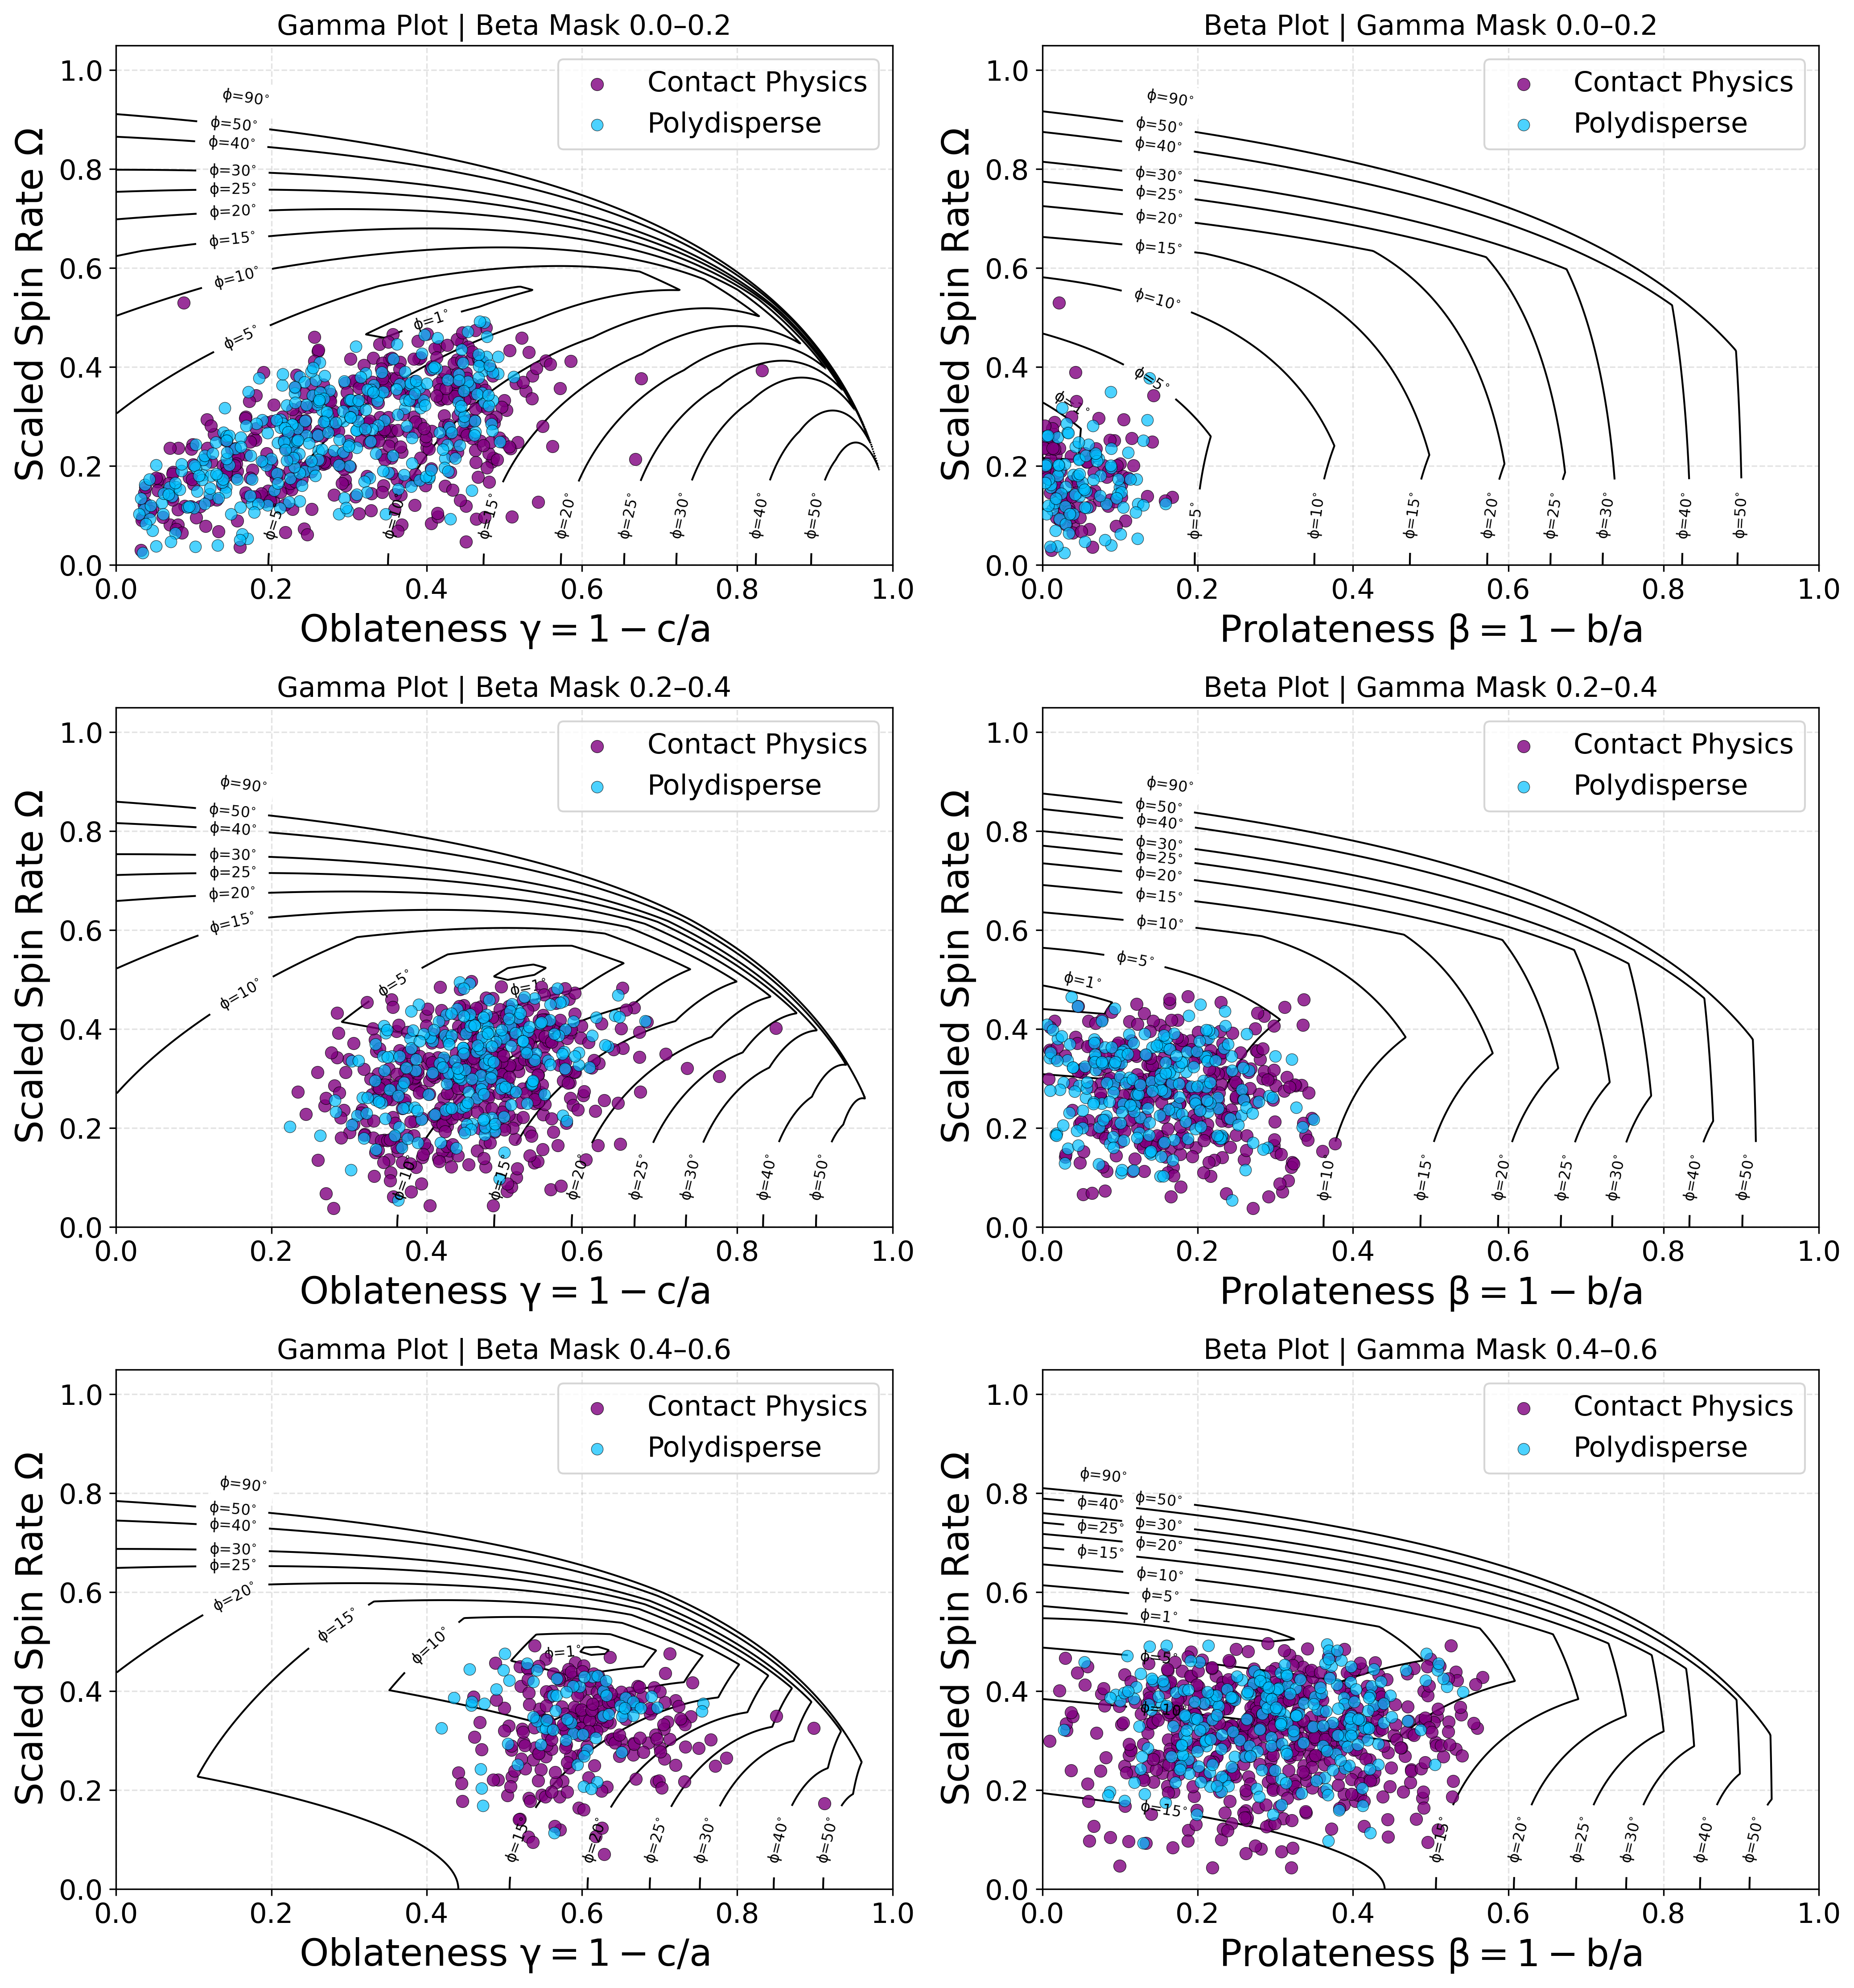
\includegraphics[width=\textwidth]{figures/contact_physics_vs_polydisperse_gamma_beta.png}
    \caption{ Normalized spin rate versus shape parameters for planetesimals formed from polydisperse particle distributions. The left column shows oblateness $\gamma = 1 - c/a$ and the right column shows prolateness $\beta = 1 - b/a$, plotted against the dimensionless spin rate $\Omega = \omega / \sqrt{\rho G}$. Each panel corresponds to a different internal friction coefficient:  $\theta = 0.1$ (top), $\theta = 0.3$ (middle), and $\theta = 0.5$ (bottom).  Blue markers represent simulations with interparticle friction, while red markers correspond to frictionless cases. Background contours indicate the internal friction angle (in degrees), providing constraints on the stability of rotating bodies with different shapes and spin rates. Increasing friction reduces shape deformation and confines the aggregates to more axisymmetric configurations, while frictionless systems show larger scatter and higher degrees of rotational elongation.}
    \label{fig:oblateness_prolateness_cp}
\end{figure*}


\subsection{Summary \& Conclusions}
The results presented in this section reveal a coherent picture of planetesimal formation through gravitational collapse, where both monodisperse and polydisperse systems share fundamental dynamical behaviors but diverge in structural and morphological details.

The shared trends, described in Section~3.1, show that regardless of particle-size uniformity, the collapse process produces a consistent spin–size relationship and similar shape–spin correlations. These outcomes are governed primarily by global angular momentum conservation and self-gravity, demonstrating that the basic dynamical pathways of collapse are robust across different material populations.

Section~3.2 highlights how particle-size diversity introduces meaningful physical differences. Polydisperse systems achieve higher bulk densities at small masses due to more efficient packing, while monodisperse systems remain more porous. Rotation period distributions further indicate that polydisperse clouds tend to form faster rotators, reflecting enhanced angular-momentum exchange during collapse. Binary formation statistics reveal a complementary trend—polydisperse clouds form fewer but more massive and tightly bound binaries, whereas monodisperse clouds produce a larger number of wider and less efficient systems. Shape and orbital analyses confirm that polydispersity leads to greater morphological and dynamical diversity, consistent with more complex collapse geometries.

Finally, Section~3.3 isolates the influence of internal friction within polydisperse populations. Increasing interparticle friction suppresses rotational deformation and promotes near-spherical equilibrium shapes, while frictionless aggregates remain more elongated and rotationally excited. This demonstrates that material strength and energy dissipation further regulate the stability of the resulting bodies, beyond the effects of particle-size variation alone.

Overall, these findings suggest that gravitational collapse establishes the fundamental dynamical framework of planetesimal formation, while particle-size diversity and frictional physics determine the fine structure, spin, and multiplicity outcomes observed in both simulations and the Solar System.

\section*{Acknowledgements}

The Acknowledgements section is not numbered. Here you can thank helpful
colleagues, acknowledge funding agencies, telescopes and facilities used etc.
Try to keep it short.

%%%%%%%%%%%%%%%%%%%%%%%%%%%%%%%%%%%%%%%%%%%%%%%%%%
\section*{Data Availability}

 
The inclusion of a Data Availability Statement is a requirement for articles published in MNRAS. Data Availability Statements provide a standardised format for readers to understand the availability of data underlying the research results described in the article. The statement may refer to original data generated in the course of the study or to third-party data analysed in the article. The statement should describe and provide means of access, where possible, by linking to the data or providing the required accession numbers for the relevant databases or DOIs.




%%%%%%%%%%%%%%%%%%%% REFERENCES %%%%%%%%%%%%%%%%%%

% The best way to enter references is to use BibTeX:

\bibliographystyle{mnras}
\bibliography{biblio} % if your bibtex file is called example.bib


% Alternatively you could enter them by hand, like this:
% This method is tedious and prone to error if you have lots of references
%\begin{thebibliography}{99}
%\bibitem[\protect\citeauthoryear{Author}{2012}]{Author2012}
%Author A.~N., 2013, Journal of Improbable Astronomy, 1, 1
%\bibitem[\protect\citeauthoryear{Others}{2013}]{Others2013}
%Others S., 2012, Journal of Interesting Stuff, 17, 198
%\end{thebibliography}

%%%%%%%%%%%%%%%%%%%%%%%%%%%%%%%%%%%%%%%%%%%%%%%%%%

%%%%%%%%%%%%%%%%% APPENDICES %%%%%%%%%%%%%%%%%%%%%

\appendix

\section{Some extra material}

If you want to present additional material which would interrupt the flow of the main paper,
it can be placed in an Appendix which appears after the list of references.

%%%%%%%%%%%%%%%%%%%%%%%%%%%%%%%%%%%%%%%%%%%%%%%%%%


% Don't change these lines
\bsp	% typesetting comment
\label{lastpage}
\end{document}

% End of mnras_template.tex
